%%% LaTeX-Vorlage Version 2.1 %%%

% TODO: individuelle Einstellungen (Name, Titel etc.)
% -> bitte in Konfigurationsdatei anpassen
\input{includes/extra/config.tex}

% Grundlegende Dokumenteneigenschaften gemäß DHBW-Vorgaben
\documentclass[a4paper,fontsize=11pt,oneside,parskip=half,headings=normal,listof=nochaptergap]{scrreprt} 
% \usepackage{showframe} % nur für Kontrolle der Ränder 

%%% Präambel einbinden (mit Festlegungen gemäß DHBW-Vorgaben) %%%
\input{template/_dhbw_praeambel.tex}

%%% Name der eigenen Literatur-Datenbank (ggf. anpassen) %%%
\bibliography{includes/literatur-datenbank.bib}

\begin{document}
%%% Deckblatt gemäß DHBW-Vorgaben einbinden (keine Anpassung nötig) %%% 
\input{template/_dhbw_deckblatt.tex}

%%% Umstellung der Seiten-Nummerierung auf i, ii, iii ... %%%
\pagenumbering{Roman} 

%%% Abstract einbinden (optionale Kurzfassung Ihrer Arbeit) %%%
\begin{abstract}
\thispagestyle{kapitelkopfzeile}
\textbf{Abstract der BA}

Dies wird meine Bachelorarbeit

Muss noch ausgefüllt werden

\end{abstract}


\cleardoublepage

%%% Inhalts-, Abbildungs-, Tabellenverzeichnisse %%%
% werden einzeilig gesetzt, um Platz zu sparen 
\begin{spacing}{1}
\tableofcontents % Inhaltsverzeichnis ausgeben
\clearpage
\startAbkVerzeichnis

\begin{acronym}[DHBW] 
% Argument definiert die Breite der ersten Spalte anhand des längsten vorkommenden Eintrags
\acro{API}{Application Programming Interface}
\acro{BFSG}{Barrierefreiheitsstärkungsgesetz}
\acro{BITBW}{IT Baden-Württemberg}
\acro{BITV}{Barrierefreie-Informa\-tionstechnik-Verordnung}
\acro{CLI}{Command Line Interface}
\acro{DSR}{Design Science Research}
\acro{DOM}{Document Object Model}
\acro{DSGVO}{Datenschutz-Grundverordnung}
\acro{EAA}{\textit{European Accessibility Act}}
\acro{FA}{Funktionale Anforderungen}
\acro{HTML}{Hypertext Markup Language}
\acro{JSON}{JavaScript Object Notation}
\acro{KI}{Künstliche Intelligenz}
\acro{LLM}{Large Language Model}
\acro{NFA}{Nicht-funktionale Anforderungen}
\acro{PoC}{Proof of Concept}
\acro{RAG}{Retrieval-Augmented Generation}
\acro{TF}{Teilfragen}
\acro{WAI}{Web Accessibility Initivative}
\acro{WCAG}{Web Content Accessibility Guidelines} 
\acro{WHO}{World Health Organization}
\end{acronym}

\vspace{2em} % Abkürzungsverzeichnis einbinden

\clearpage
\thispagestyle{kapitelkopfzeile}
\listoffigures
\phantomsection
\addcontentsline{toc}{chapter}{\listfigurename} % Abb.verz. ins Inh.verz. aufnehmen

\clearpage
\listoftables
\phantomsection
\addcontentsline{toc}{chapter}{\listtablename} % Tab.verz. ins Inh.verz. aufnehmen
\end{spacing}

%%% Umstellung der Seiten-Nummerierung auf 1, 2, 3 ... %%%
\cleardoublepage
\pagenumbering{arabic}

%%% Ihr eigentlicher Inhalt %%%
% Empfehlung: strukturieren Sie Ihren Text in einzelnen Dateien 
% und binden Sie diese hier mit \input{includes/dateiname.tex} ein
\chapter{Einleitung} \label{kap:1}

Digitale Anwendungen sind für Verwaltung, Wirtschaft und Gesellschaft zu einer zentralen Infrastruktur geworden. Hinsichtlich dieser Entwicklung gewinnt Web-Barrierefreiheit zunehmend an Bedeutung, damit alle Menschen - unabhängig von individuellen Einschränkungen - gleichberechtigten Zugang zu digitalen Informationen und Dienstleistungen erhalten. In der Praxis zeigt sich jedoch eine Diskrepanz zwischen normativen Anforderungen (z. B. \ac{WCAG}-basierte Kriterien)\footcite[Vgl.][]{WCAG} und der tatsächlichen Umsetzung in Softwareprojekten: Barrierefreiheit wird häufig spät berücksichtigt, Prüfungen erfolgen punktuell und Korrekturen sind zeitaufwendig. Besonders in gewachsenen Systemlandschaften mit Legacy-Anteilen und knappen Entwicklungsressourcen entstehen so immer wieder Qualitätsdefizite.

Parallel dazu haben sich \ac{LLM}s als leistungsfähige Werkzeuge zur Unterstützung von Softwareentwicklung etabliert. Sie helfen, Aufgaben wie Code-Analyse, Refactoring oder die Erstellung technischer Empfehlungen zu beschleunigen. Für die Barrierefreiheit ist dies besonders relevant: Hier müssen nicht nur Fehler erkannt, sondern auch korrekt, standardkonform und kontextsensitiv behoben werden. Gleichzeitig bestehen in vielen Organisationen, insbesondere in sensiblen Umgebungen, strikte Vorgaben an Datenschutz und Informationssicherheit, wodurch Cloud-basierte Assistenzsysteme häufig nicht eingesetzt werden dürfen. Daraus ergibt sich die zentrale Herausforderung, \ac{LLM}-Unterstützung so zu gestalten, dass sie lokal, nachvollziehbar und qualitätsgesichert in bestehende Entwicklungsprozesse integriert werden kann.

Diese Arbeit untersucht daher, wie ein \ac{LLM}- bzw. agentenbasierter Ansatz zur automatisierten Erkennung und Behebung von Barrierefreiheitsproblemen in Webanwendungen konzipiert und prototypisch umgesetzt werden kann.\footcite[Vgl.][S. 297]{bassi_assessment_2025} Im Fokus steht ein Workflow, der automatisierte Tests (z. B. via Browser-Automation und Accessibility-Linter) mit einer \ac{LLM}-gestützten Analyse und Änderungsvorschlägen verbindet und die Änderungen anschließend erneut testet. Ziel ist es, den manuellen Aufwand zu reduzieren, die Konsistenz der Ergebnisse zu erhöhen und Barrierefreiheit als kontinuierlichen Bestandteil der Softwarequalität zu verankern.

\section{Motivation und Kontext}

Rund 1,3 Milliarden Menschen (16\% der Weltbevölkerung) leben mit einer Form von Behinderung.\footcite[Vgl.][]{WHO} Für diese Personengruppe ist der Zugang zu digitalen Angeboten keine bloße Komfortfrage, sondern eine Voraussetzung für gesellschaftliche Teilhabe in nahezu allen Lebensbereichen: von der Kommunikation mit Behörden über den Zugang zu Bildung und Gesundheitsinformationen bis hin zur Teilnahme am wirtschaftlichen Leben. Das Recht auf barrierefreien Zugang zu Informations- und Kommunikationstechnologien ist völkerrechtlich in der UN-Behindertenrechtskonvention verankert und hat sich in den vergangenen Jahren zunehmend auch in verbindlichem nationalen und europäischen Recht niedergeschlagen.\footcite[Vgl.][]{OHCHR}

Auf europäischer Ebene verpflichtet der \ac{EAA} die Mitgliedstaaten, Barrierefreiheitsanforderungen für digitale Produkte und Dienstleistungen durchzusetzen.\footcite[Vgl.][]{EAA} In Deutschland wurde diese Richtlinie durch das \ac{BFSG} in nationales Recht überführt, das seit dem 28. Juni 2025 auch für weite Teile der Privatwirtschaft gilt.\footcite[Vgl.][]{BFSG} Ergänzt wird dieser Rahmen durch die \ac{BITV}, die für Behörden und öffentliche Stellen bereits seit Jahren verbindliche Vorgaben formuliert.\footcite[Vgl.][S. 281]{BITV, heinemann_barrierefreiheit_2024}

Trotz dieser eindeutigen Rechtslage ist die praktische Umsetzung barrierefreier Webanwendungen nach wie vor unzureichend. Die jährlich durchgeführte WebAIM-Million-Studie, die die Startseiten der meistbesuchten Webseiten weltweit analysiert, stellte 2025 fest, dass 94,8\% der untersuchten Seiten nachweisbare Verstöße gegen die \ac{WCAG} aufweisen.\footcite[Vgl.][]{WebAIM} Damit bleibt Barrierefreiheit in der Entwicklungspraxis trotz gesetzlicher Verpflichtung systematisch unterrepräsentiert. Im Vergleich mit den letzten Jahren ist seit 2019 (97,8\%) lediglich eine Verbesserung um 3 Prozentpunkte zu verzeichnen.\footcite[Vgl.][]{WebAIM19}

Die \ac{BITBW} nimmt als zentrale IT-Dienstleisterin der Landesverwaltung Baden-Württemberg in diesem Kontext eine besondere Stellung ein.\footcite[Vgl.][]{BITBW_2021} Als Entwicklerin und Betreiberin öffentlicher Webanwendungen für Ministerien, Polizeibehörden und Kommunen ist sie gesetzlich zur Einhaltung der \ac{BITV} und des \ac{BFSG} verpflichtet.\footcite[Vgl.][]{Landesrecht_BW} Drei Faktoren machen die \ac{BITBW} zu einem besonders geeigneten Praxiskontext für die vorliegende Arbeit: Erstens unterliegen ihre Anwendungen strengeren Barrierefreiheitsanforderungen als privatwirtschaftliche Produkte. Zweitens schließen die Datenschutzvorgaben der öffentlichen Verwaltung die Nutzung cloudbasierter \ac{LLM}-\ac{API}s weitgehend aus. Drittens erschweren gewachsene Systemlandschaften mit Legacy-Anteilen und begrenzten Entwicklungsressourcen die manuelle Barrierefreiheitsprüfung im erforderlichen Umfang. Sie bildet damit den praktischen Rahmen der vorliegenden Arbeit.

\section{Problemstellung}

Die mangelhafte Umsetzung von Barrierefreiheit in Softwareprojekten lässt sich nicht allein auf fehlende Motivation oder Ressourcen zurückführen. Ein wesentlicher Treiber sind die Schwächen der verfügbaren Werkzeuge und Tools: Automatisierte Barrierefreiheitsanalyse-Tools wie axe\footcite[Vgl.][]{axe}, WAVE\footcite[Vgl.][]{WAVE} oder Lighthouse\footcite[Vgl.][]{Lighthouse} erkennen zwar syntaktische Verstöße, stoßen jedoch bei semantischen Problemen an ihre Grenzen. Ob ein vorhandener Alternativtext den Bildinhalt tatsächlich angemessen beschreibt, oder ob eine Schaltflächenbeschriftung für Screenreader-Nutzerinnen und -Nutzer verständlich ist, entzieht sich der regelbasierten Prüflogik dieser Werkzeuge.

Empirisch belegt wird diese Schwäche durch das Mutation-Testing-Framework \textfett{Ma11y}: In einer systematischen Evaluation mit 25 gezielt eingebrachten Barrierefreiheits-Defekten erkannte kein einzelnes der sechs untersuchten Tools mehr als 50\% der injizierten Fehler. Somit blieben im Durchschnitt nahezu die Hälfte aller Defekte unentdeckt.\footcite[Vgl.][S. 100]{tafreshipour_ma11y_2024} Besonders aufschlussreich ist dabei die Differenzierung nach Verstoßtypen: Während syntaktische Defekte zu 54\% erkannt wurden, lag die Erkennungsrate bei semantischen Verstößen lediglich bei 26\%.\footcite[Vgl.][S. 108]{tafreshipour_ma11y_2024} Sechs der 25 Defekttypen - darunter die Manipulation von Seitentiteln und Alternativtexten - wurden von keinem der untersuchten Tools erkannt.

Eine zweite strukturelle Schwäche betrifft die Charakteristik moderner Webanwendungen. Rich-Client-Anwendungen auf Basis von Frameworks wie React erzeugen ihren Inhalt größtenteils clientseitig und verändern den \ac{DOM} dynamisch in Abhängigkeit von Nutzerinteraktionen. Die zunehmende Komplexität solcher Webanwendungen ist im Anhang veranschaulicht (vgl. Abbildung \ref{fig:complexity}). Barrieren entstehen häufig erst in bestimmten Zuständen: wenn ein Modalfenster geöffnet wird, eine Fehlermeldung erscheint oder ein Dropdown-Menü aktiviert ist. Rein statische Analysen - oder Analysen, die ausschließlich den initialen Seitenladezustand prüfen - erfassen diese zustandsabhängigen Barrieren nicht.\footcite[Vgl.][S. 303]{bassi_assessment_2025}

Jüngere Forschungsarbeiten zeigen, dass \ac{LLM}s geeignet sind, die Grenzen regelbasierter Tools zu überwinden. So erreicht das System \textfett{AccessGuru}durch den Einsatz von GPT-4o eine Reduktion des Violation Scores um bis zu 84\%\footcite[Vgl.][]{fathallah_accessguru_2025}, und \textfett{GenA11y} erzielt bei der Erkennung von Barrierefreiheitsproblemen eine Precision von 94,5\%\footcite[Vgl.][FSE101:1]{he_enhancing_2025}. Diese Ansätze beschränken sich jedoch auf statisches \ac{HTML}. Keiner der bekannten Ansätze verknüpft Tool-Reports, Playwright-\allowbreak Interaktionsdaten und den Quellcode der geprüften Komponenten zu einem integrierten Analysesystem.\footcite[Vgl.][]{fathallah_accessguru_2025} Der Schritt von der Fehlererkennung zu einer entwicklernahen, direkt umsetzbaren Handlungsempfehlung - idealerweise mit Bezug zur konkreten Quellcodestelle - wird in der Literatur zwar als offenes Problem benannt,\footcite[Vgl.][FSE101:15-17]{he_enhancing_2025} bleibt aber bislang ungelöst.

Daraus ergibt sich eine klar umrissene Lücke: Es fehlt ein Assistenzsystem, das (a) die dynamischen Zustände einer React-Anwendung durch automatisierte Browser-Interaktionen erfasst, (b) die Ergebnisse automatisierter Tool-Reports mit dem relevanten Quellcode verknüpft und (c) auf dieser Grundlage priorisierte, entwicklernahe Handlungsempfehlungen erzeugt - lokal ausführbar und ohne den Transfer sensibler Anwendungsdaten an externe Dienste.

\section{Zielsetzung und Forschungsfragen} \label{kap:1.3}

Ziel dieser Bachelorarbeit ist die Konzeption und prototypische Umsetzung einer lokal ausführbaren, kontextsensitiven Assistenzlösung zur Barrierefreiheitsanalyse von Rich-Client-Web\-an\-wen\-dun\-gen. Als Untersuchungsobjekt dient eine React-basierte Webanwendung aus dem Umfeld der \ac{BITBW}. Der Proof of Concept soll automatisierte Barrierefreiheits-Reports, Interaktionsdaten aus Playwright-\allowbreak Tests sowie ausgewählte Informationen aus der Codebasis in einer Datenpipeline zusammenführen. Auf dieser Grundlage werden priorisierte, entwicklernahe Handlungsempfehlungen abgeleitet und strukturiert aufbereitet.

Die Arbeit liefert drei konkrete Beiträge: Erstens einen strukturierten Überblick darüber, wie unterschiedliche Datenquellen der Barrierefreiheitsanalyse systematisch kombiniert und interpretiert werden können. Zweitens einen Proof of Concept, der das Vorgehen exemplarisch demonstriert. Drittens eine qualitative Evaluation anhand definierter Kriterien, die aus den Anforderungen und der einschlägigen Fachliteratur abgeleitet werden.

Die übergeordnete Forschungsfrage dieser Arbeit lautet:

\textfett{Inwieweit kann ein kontextsensitives KI-Assistenzsystem, das Tool-Reports, Play\-wright-Inter\-aktions\-daten und Quellcode kombiniert, Barrierefreiheitsverstöße in Re\-act-ba\-sier\-ten Webanwendungen automatisiert erkennen und entwicklernahe Handlungsempfehlungen generieren?}

Diese übergeordnete Frage wird durch zwei konkretisierende \ac{TF} operationalisiert:
\begin{itemize}
    \item \ac{TF}1: Welche Typen von Barrierefreiheitsverstößen - syntaktisch, semantisch und layout-bezogen - lassen sich durch den gewählten Ansatz zuverlässig erkennen, und wo liegen die methodischen Grenzen?
    \item \ac{TF}2: Inwiefern verbessert die Einbeziehung von Quellcode und Playwright-\allowbreak Interaktionsdaten die Qualität der generierten Handlungsempfehlungen gegenüber rein \ac{DOM}-basierten Ansätzen?
\end{itemize}

\ac{TF}1 adressiert dabei das Erkennungsproblem und erlaubt eine differenzierte Aussage über die Leistungsfähigkeit und Grenzen des Systems entlang der Verstoß-Taxonomie von Fathallah et al.\footcite[Vgl.][S. 114-115]{fathallah_accessguru_2025, Šmite_Wohlin_Galviņa_Prikladnicki_2012} \ac{TF}2 greift den in der Literatur identifizierten Mehrwert der Quellcode-Kontextualisierung auf und überprüft ihn im Rahmen einer qualitativen Evaluation am gewählten Untersuchungsobjekt.

\section{Aufbau der Arbeit}

Die vorliegende Arbeit gliedert sich in acht Kapitel. Im Anschluss an die Einleitung werden in Kapitel \ref{kap:2} die theoretischen Grundlagen erarbeitet: Barrierefreiheit im Web, die \ac{WCAG}-Standards und der rechtliche Rahmen, die Charakteristika von Rich-Client-Web\-an\-wen\-dun\-gen sowie Grundlagen zu Large Language Models und Prompt-Engineering-Strategien.

Kapitel \ref{kap:3} gibt einen systematischen Überblick über den Stand der Forschung. Die relevanten Arbeiten werden thematisch gegliedert - nach \ac{LLM}-basierter Erkennung, Code-Korrektur, hybriden Pipelines und Evaluation - und in einer Konzeptmatrix nach Webster und Watson zusammengefasst.\footcite[Vgl.][]{WebsterWatson2002} Das Kapitel schließt mit einer expliziten Einordnung des Beitrags der vorliegenden Arbeit.

Kapitel \ref{kap:methodik} legt das methodische Vorgehen dar. Es beschreibt die Wahl des Design-Science-Research-Paradigmas als wissenschaftliche Methode, definiert den Untersuchungsgegenstand und entwirft das Evaluationsdesign.\footcite[Vgl.][]{hevner2004dsr} Kapitel \ref{kap:4} analysiert den Problemkontext und leitet daraus funktionale und nicht-funktionale Anforderungen ab, einschließlich der Begründung der Modellauswahl.

Auf Basis dieser Anforderungen wird in Kapitel \ref{kap:5} das Assistenzsystem konzipiert: Systemarchitektur, Datenpipeline, Prompt-Strategie und Ausgabeformat werden begründet entworfen. Kapitel \ref{kap:6} beschreibt die prototypische Implementierung des Proof of Concept und illustriert die Systemfunktionalität anhand von Beispielabläufen für syntaktische, semantische und dynamisch erzeugte Barrierefreiheitsprobleme.

Kapitel \ref{kap:7} präsentiert und diskutiert die Evaluationsergebnisse, beantwortet die Forschungsfragen und reflektiert die Limitationen des Ansatzes. Das abschließende Kapitel \ref{kap:8} fasst die Kernaussagen zusammen, ordnet den Beitrag der Arbeit in die Forschungslandschaft ein und formuliert Empfehlungen für weiterführende Untersuchungen.
\chapter{Theoretische Grundlagen} \label{kap:2}

Das folgende Kapitel legt die theoretischen Grundlagen für die Konzeption des Proof of Concept dar. Es werden Begriffe und Konzepte erläutert, die für das Verständnis der Problemstellung und des entwickelten Ansatzes erforderlich sind. Zunächst wird Barrierefreiheit im Web als Untersuchungsgegenstand definiert (Abschnitt \ref{kap:2.1}), anschließend der Stand automatisierter Barrierefreiheitstools sowie ihre Möglichkeiten und Grenzen (Abschnitt \ref{kap:2.2}). Darauf aufbauend werden dann die besonderen Herausforderungen von Rich-Client-Anwendungen und das Werkzeug Playwright eingeführt (Abschnitt \ref{kap:2.3}). Das Kapitel schließt mit einer Einführung in \acs{LLM}, Modelle und relevante Prompting-Strategien sowie Datenschutzaspekte (Abschnitt \ref{kap:2.4}).

\section{Barrierefreiheit von Webanwendungen} \label{kap:2.1}

\subsection{Begriffsdefinition und Relevanz}

Der Begriff \textit{Web Accessibility}, im Deutschen Web-Barrierefreiheit, bezeichnet nach Definition der \ac{WAI} die Eigenschaft von Webangeboten, von allen Menschen unabhängig von körperlichen, motorischen oder sensorischen Einschränkungen sowie individuellen Fähigkeiten wahrgenommen, bedient und genutzt werden zu können.\footcite[Vgl.][S. 172]{abuaddousWebAccessibilityChallenges2016} Web Accessibility geht jedoch über die reine Wahrnehmbarkeit hinaus und umfasst auch die Bedienbarkeit sowie Nutzbarkeit von Webangeboten.\footcite[Vgl.][]{WAI} Laut Angaben der \ac{WHO} wird geschätzt, dass rund 16\% der Weltbevölkerung mit einer Form von Behinderung leben.\footcite[Vgl.][]{WHO} Diese Zahl umfasst ein breites Spektrum an Einschränkungen, von denen nicht alle die Nutzung digitaler Angebote unmittelbar betreffen. Entscheidend für die Web-Barrierefreiheit sind vor allem visuelle, motorische und kognitive Beeinträchtigungen, die die Wahrnehmung oder Bedienung digitaler Oberflächen erschweren. Damit stellt Barrierefreiheit im Web nicht nur eine technische Herausforderung dar, sondern auch eine zentrale gesellschaftliche Aufgabe zur Gewährleistung digitaler Teilhabe. Das Recht auf barrierefreien Zugang zu Informations- und Kommunikationstechnologien ist seit 2006 in Art. 9 der UN-Behindertenrechtskonvention völkerrechtlich verankert.\footcite[Vgl.][S. 9]{OHCHR}

In der Forschungsliteratur werden vier wesentliche Behinderungsformen unterschieden, die jeweils spezifische Anforderungen an die Gestaltung barrierefreier Webangebote stellen.\footcite[Vgl.][S. 493--494]{ResearchMethodsHumanComputer2017} Für diese Arbeit sind insbesondere zwei Kategorien relevant -- visuelle Beeinträchtigungen und motorische Einschränkungen --, da sie den Großteil der automatisiert prüfbaren \ac{WCAG}-Verstöße betreffen:

\textfett{Visuelle Beeinträchtigungen} umfassen vollständige oder partielle Blindheit sowie Farbfehlsichtigkeit.\footcite[Vgl.][]{gubbi_mohanbabu_context-aware_2024} Betroffene Personen nutzen häufig Screenreader-Software (z.\,B. JAWS, NVDA, VoiceOver), die auf eine korrekte semantische \ac{HTML}-Struktur angewiesen ist.\footcite[Vgl.][S. 5508]{morrisMostItBeing2016} Fehlende Alternativtexte, unzureichende Farbkontraste und fehlende \texttt{aria}-Labels bilden die häufigsten Verstöße in dieser Kategorie\footcite[Vgl.][Erfolgskriterium 1.1.1]{WCAG} und zugleich den primären Erkennungsbereich des in dieser Arbeit entwickelten Systems.

\textfett{Motorische Einschränkungen} betreffen Personen, die konventionelle Eingabegeräte wie Maus oder Touchscreen nicht präzise bedienen können.\footcite[Vgl.][S. 110381--110382]{perezLongitudinalStudyTwo2020} Sie sind auf Tastaturnavigation, Sprachsteuerung oder spezielle assistive Eingabegeräte angewiesen.\footcite[Vgl.][S. 208]{kouroupetroglouAssistiveTechnologiesComputer01} Eine vollständige Bedienbarkeit über die Tastatur ist daher eine zentrale Voraussetzung für barrierefreie Nutzung.\footcite[Vgl.][]{WebAIMKeyboardAccessibility} Für das vorliegende System ist diese Kategorie besonders relevant, da Tastaturfallen und fehlende Fokussteuerung in (React-)Anwendungen häufig erst durch interaktionsbasierte Tests -- etwa mittels Playwright -- aufgedeckt werden können.\footcite[Vgl.][S. 855]{chiou_detecting_2021}

Daneben adressiert die \ac{WCAG} auch auditive und kognitive Beeinträchtigungen; beide erfordern jedoch überwiegend menschliches Urteilsvermögen und entziehen sich weitgehend der automatisierten Prüfung -- sie liegen daher außerhalb des Scopes des vorliegenden \ac{PoC}.\footcite[Vgl.][]{abou-zahra_artificial_2018}

Assistive Technologien -- darunter Screenreader, Bildschirmvergrößerungssoftware und alternative Eingabegeräte -- bilden die technische Voraussetzung für die Nutzung digitaler Angebote durch die genannten Personengruppen.\footcite[Vgl.][]{WAI, abou-zahra_artificial_2018} Ihre Wirksamkeit hängt jedoch unmittelbar davon ab, dass Webanwendungen klar definierte strukturelle und semantische Anforderungen erfüllen.\footcite[Vgl.][S. 82]{morrisonImaginingArtificialIntelligence2017} Die Nichterfüllung dieser Anforderungen führt nicht nur zu einer Beeinträchtigung der betroffenen Personen, sondern kann auch wirtschaftliche und rechtliche Konsequenzen nach sich ziehen.\footcite[Vgl.][S. 864--865]{krok_digital_2024}

\subsection{\ac{WCAG}: Aufbau, Prinzipien und Konformitätsstufen}

Die \acs{WCAG} sind der internationale Standard für barrierefreie Webinhalte und werden vom \ac{W3C} im Rahmen der \ac{WAI} veröffentlicht. Die derzeit maßgebliche Referenzversion ist \ac{WCAG} 2.2, die im Oktober 2023 \ac{WCAG} 2.1 (2018) als aktuelle Referenzversion ablöste.\footcite[Vgl.][]{WCAG2.1,WCAG} \ac{WCAG} 2.2 führt neun zusätzliche Erfolgskriterien ein und berücksichtigt insbesondere kognitive Einschränkungen und mobile Nutzung.\footcites[Vgl.][S. 118]{PolicyPracticeSystematic2025}[Vgl.][]{souzaAccessibilityEvaluationWeb2024} Zu diesen Kriterien gehören konsistentere Fokusindikatoren (2.4.11--2.4.13) und die Vermeidung von Drag-and-Drop-Pflichtinteraktionen (\ac{WCAG} 2.5.7).\footcite[Vgl.][]{WCAG}

Die \ac{WCAG} ist in vier Schichten gegliedert: Prinzipien, Richtlinien, Erfolgskriterien und unterstützende Techniken. Auf oberster Ebene stehen vier grundlegende Prinzipien, 
zusammengefasst im Akronym \textbf{POUR}: \textit{Perceivable} (Wahrnehmbarkeit), \textit{Operable} (Bedienbarkeit), \textit{Understandable} (Verständlichkeit) und \textit{Robust} (Robustheit).\footcite[Vgl.][]{souzaAccessibilityEvaluationWeb2024} Typische Anforderungen sind Alternativtexte für Bilder (1.1.1), ausreichende Farbkontraste (1.4.3) und vollständige Tastaturerreichbarkeit aller Funktionen.\footcite[Vgl.][Abschnitte 1--4]{WCAG}

Die 13 Richtlinien unterhalb der Prinzipien werden durch insgesamt 87 testbare Erfolgskriterien operationalisiert (\ac{WCAG} 2.2; gegenüber 78 in \ac{WCAG} 2.1 kommen neun neue Kriterien hinzu, während SC~4.1.1 als obsolet markiert wird).\footcite[Vgl.][]{WCAG} Jedes Erfolgskriterium ist einer von drei Konformitätsstufen zugeordnet.\footcite[Vgl.][]{fathallah_accessguru_2025} Stufe A umfasst grundlegende Anforderungen, deren Nichteinhaltung bestimmte Nutzergruppen vollständig ausschließt. Stufe AA ist der in Europa gesetzlich geforderte Mindeststandard für öffentliche Stellen und weitere Teile der Privatwirtschaft.\footcite[Vgl.][S. 40, 195 ff.]{kerkmann_barrierefreie_2015} Stufe AAA beschreibt Anforderungen, die nicht für alle Inhalte generell erfüllbar sind. Die vorliegende Arbeit fokussiert sich entsprechend dem gesetzlichen Mindeststandard auf Stufe A und AA.

\begin{figure}[htbp]
  \centering
  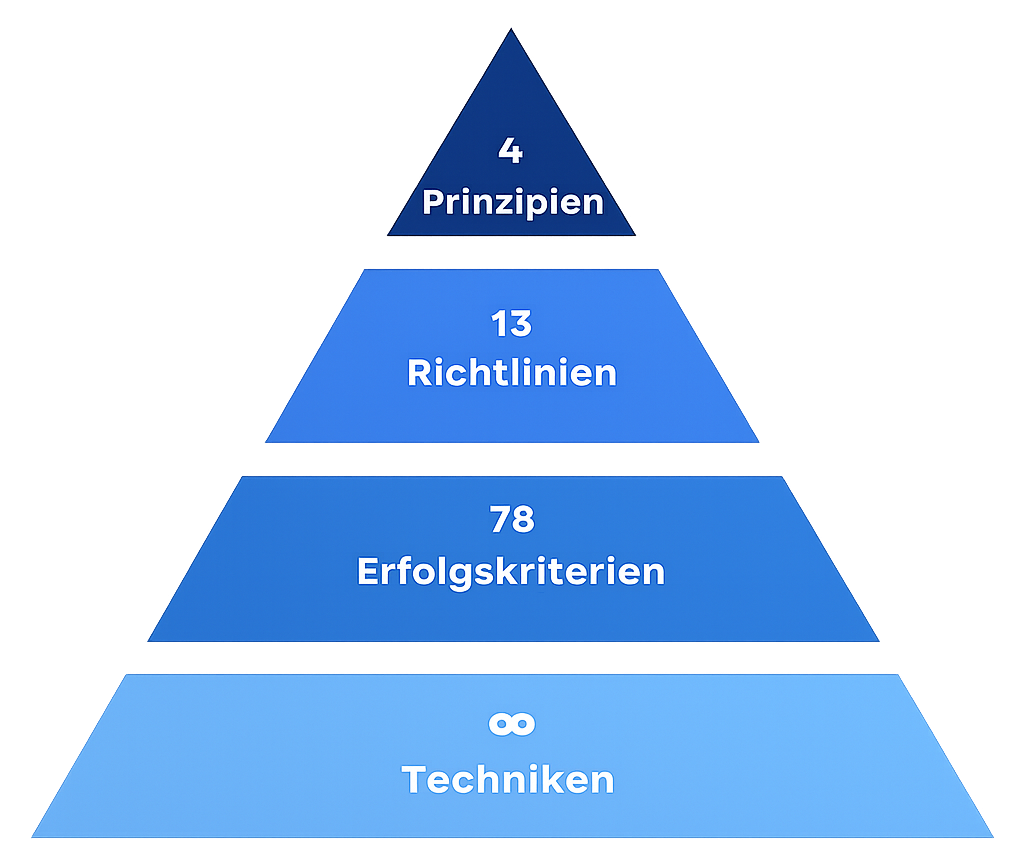
\includegraphics[width=0.4\textwidth]{graphics/WCAG-Dreieck-4-Ebenen.png}
 \caption[\ac{WCAG}-Schichtenmodell]{\ac{WCAG}-Schichtenmodell\protect\footnote{Eigene Abbildung}}
  \label{fig:WCAG-Schichten}
\end{figure}

Die praktische Umsetzung dieser Standards ist trotz ihrer langen Existenz nach wie vor unzureichend.\footcite[Vgl.][S. 297]{bassi_assessment_2025} Die WebAIM-Million-Studie 2025 identifizierte durchschnittlich 56,8 \ac{WCAG}-Fehler pro Seite. Die häufigsten Verstoßkategorien betrafen fehlende Alternativtexte (54,5\%), unzureichende Farbkontraste (80,6\%), fehlende Labels (47,4\%), leere Links (44,6\%) und fehlende Sprachangaben im \ac{HTML} (17,1\%).\footcite[Vgl.][]{WebAIM}

\subsection{Rechtlicher Rahmen}

Auf europäischer Ebene bildet der \acf{EAA} den übergeordneten rechtlichen Rahmen.\footcite[Vgl.][]{EAA} Er verpflichtet die Mitgliedstaaten, Barrierefreiheitsanforderungen für digitale Produkte und Dienstleistungen einheitlich durchzusetzen.

In Deutschland wird der \ac{EAA} durch das \acf{BFSG} in nationales Recht überführt.\footcite[Vgl.][]{BFSG} Das \ac{BFSG} ist seit dem 28. Juni 2025 für privatwirtschaftliche Anbieter verbindlich. Unternehmen mit weniger als zehn Beschäftigten und einem Jahresumsatz unter zwei Millionen Euro sind von bestimmten Pflichten ausgenommen.\footcite[Vgl.][§1 (Anwendungsbereich) und §3 (Barrierefreiheit)]{BFSGGesetz}

Für öffentliche Stellen des Bundes gilt in Deutschland bereits seit 2011 die \acf{BITV} 2.0, die Behörden verpflichtet, ihre Webangebote nach \ac{WCAG} 2.1 auf mindestens Konformitätsstufe AA zu gestalten und zu dokumentieren.\footcite[Vgl.][]{BITV} Die \ac{BITV} 2.0 verweist in ihrer Anlage 1 unmittelbar auf die \ac{WCAG}-Erfolgskriterien und ist damit an deren Weiterentwicklung gekoppelt.

Diese rechtlichen Anforderungen sind für alle betroffenen Organisationen verbindlich -- öffentliche Stellen ebenso wie privatwirtschaftliche Anbieter im Geltungsbereich des \ac{BFSG}. Die \acf{BITBW} als zentrale IT-Dienstleisterin der Landesverwaltung Baden-Württembergs ist davon in besonderem Maße betroffen, da sämtliche von ihr entwickelten oder betriebenen Anwendungen den Anforderungen entsprechen müssen.\footcite[Vgl.][]{BITV} Dies begründet das praktische Interesse an effizienten, automatisierten Methoden der Barrierefreiheitsüberprüfung, wie sie in dieser Arbeit untersucht werden.


\section{Automatisierte Barrierefreiheitsanalyse} \label{kap:2.2}

Trotz klar definierter \ac{WCAG}-Richtlinien wird Barrierefreiheit in der Webentwicklung häufig nur unzureichend umgesetzt. Ein zentraler Grund dafür liegt in den Entwicklungsprozessen moderner Webanwendungen. In vielen Softwareprojekten wird Barrierefreiheit nicht von Beginn an als integraler Bestandteil der Entwicklung berücksichtigt, sondern erst in späten Testphasen oder gar nicht adressiert. Hinzu kommt, dass viele Entwicklerinnen und Entwickler nur begrenztes Wissen über die \ac{WCAG}-Anforderungen besitzen und Accessibility-Aspekte nicht automatisch berücksichtigt werden.\footcite[Vgl.][S. 298]{bassi_assessment_2025} In Kombination mit Zeitdruck und fehlenden automatisierten Prüfverfahren führt dies dazu, dass Accessibility-Probleme häufig erst spät erkannt oder vollständig übersehen werden.\footcite[Vgl.][S. 123]{mowar_accessibility_2024}

\subsection{Klassische Tool-Ansätze} \label{tools}

Für die automatisierte Überprüfung von Webanwendungen auf Barrierefreiheit existiert eine stetig wachsende Zahl von Werkzeugen. Die \ac{WAI} führt in ihrer aktuellen Evaluation-Tool-Liste über 160 Werkzeuge\footcite[Vgl.][]{WAITools}, von denen 84 explizit die \ac{WCAG} 2.1 adressieren.\footcite[Vgl.][]{delnevo_interaction_2024}
Alle gängigen Werkzeuge arbeiten regelbasiert, d.\,h. sie prüfen den \ac{DOM} einer geladenen Seite anhand eines vordefinierten Regelkatalogs gegen bekannte Verstoßmuster.\footcites[Vgl.][]{kodithuwakku_assessing_2025}[][3:9]{manca_transparency_2023}
Das \acf{DOM} ist eine vom Browser erzeugte, baumartige Objektstruktur, die den \ac{HTML}-Code einer Webseite als hierarchische Struktur aus Elementknoten repräsentiert und über Programmierschnittstellen von Skripten und Analysewerkzeugen zugänglich macht.\footcite[Vgl.][]{Robie}

Zu den meistgenutzten automatisierten Barrierefreiheitstools gehören:
\begin{itemize}
    \item \textbf{axe-core}, entwickelt von Deque Systems, hat sich als Standardlösung für die automatische Integration von Accessibility-Tests in Entwicklungspipelines etabliert.\footcite[Vgl.][]{axe}
    \item \textfett{WAVE} (WebAIM) bietet visuelle Browser-Extensions, die Fehler direkt in der gerenderten Seitenansicht annotieren.\footcite[Vgl.][]{WAVE}
    \item \textfett{Lighthouse} ist in die Chrome-DevTools integriert und kombiniert Accessibility-Testing mit Performance- und SEO-Analysen.\footcite[Vgl.][]{Lighthouse}
    \item \textfett{IBM Equal Access Checker} und \textfett{ARC Toolkit} (TPGi) runden das Spektrum verbreiteter Werkzeuge ab.
\end{itemize}

Der typische Output solcher Werkzeuge ist ein strukturierter Violation Report, bei dem jedem erkannten Verstoß eine Bezeichnung, Beschreibung und ein Schweregrad zugewiesen wird (bei axe-core: minor, moderate, serious, critical) sowie, falls möglich, ein \ac{HTML}-Ausschnitt des betroffenen Elements.\footcites[Vgl.][]{kodithuwakku_assessing_2025}[][]{axe} Dieser standardisierte Output bildet in der vorliegenden Arbeit die Grundlage für die erste Stufe der Datenpipeline.

\subsection{Grenzen bestehender Tools} \label{kap:grenzen Tools}

Trotz ihrer weiten Verbreitung weisen regelbasierte Accessibility-Tools fundamentale Grenzen auf. Diese lassen sich in drei Kategorien einteilen: begrenzte Regelabdeckung, semantische Blindheit und fehlende Dynamik.

Die Regelabdeckung der Werkzeuge ist erheblich geringer als oftmals angenommen. Kodithuwakku und Wickramaarachchi zeigen, dass selbst die leistungsfähigsten untersuchten Tools lediglich 21\% aller \ac{WCAG}-Tests automatisiert abdecken können (vgl. Tabelle \ref{tab:tool_evaluation}).\footcite[Vgl.][]{kodithuwakku_assessing_2025} Die in der Tabelle ausgewiesenen Werte CER und ICR messen davon abweichende Dimensionen: CER beschreibt, welcher Anteil der tatsächlich gemeldeten Befunde korrekt ist (Präzision), während ICR angibt, wie viele der vorhandenen Probleme vom Tool gefunden wurden (Recall). Für Tastaturzugänglichkeit und auditive Barrieren lag die Erkennungsrate in ihrer Studie bei null Prozent; hinzu kommt eine hohe Rate an \textit{False Positives}.\footcite[Vgl.][]{kodithuwakku_assessing_2025} Bassi et al. kommen zu dem Ergebnis, dass das beste verfügbare Einzeltool (\textfett{ARC Toolkit}) nur 26\% der \ac{WCAG}-Tests abdeckt.\footcite[Vgl.][S. 298]{bassi_assessment_2025}%
% KÜRZUNG: Fussnote zur eingeschränkten Vergleichbarkeit der beiden Studien auf einen Satz gekürzt.
\footnote{Die Vergleichbarkeit beider Studien ist eingeschränkt, da unterschiedliche Testkorpora und Methodiken verwendet werden; die übereinstimmende Kernaussage -- regelbasierte Tools decken nur einen Bruchteil aller prüfbaren \ac{WCAG}-Kriterien ab -- ist dennoch robust.}
Die Kombination mehrerer Tools in einem Ensemble verbessert die Abdeckung, beseitigt das strukturelle Problem jedoch nicht vollständig. Pool zeigt, dass selbst ein Ensemble aus acht gleichzeitig eingesetzten Tools, darunter auch \textfett{axe-core}, \textfett{WAVE} und \textfett{Qualweb}, erhebliche Lücken hinterlässt: jedes einzelne Tool erkennt mindestens sieben Violations exklusiv, die von keinem anderen Tool gefunden werden.\footcite[Vgl.][]{pool_testaro_2023} Manca et al. stellen zudem fest, dass von elf untersuchten Werkzeugen lediglich drei explizit auf ihre Erkennungslücken hinweisen.\footcite[Vgl.][S. 4]{manca_transparency_2023}


\begin{table}[htbp]
\centering
\small
\begin{tabular}{lcccc}
\toprule
\textbf{Tool} & \textbf{True Positives} & \textbf{False Positives} & \textbf{CER (\%)} & \textbf{ICR (\%)} \\
\midrule
Lighthouse & 17 & 16 & 52.94 & 15.92 \\
WAVE & 16 & 12 & 35.29 & 14.65 \\
SiteImprove & 23 & 18 & 47.06 & 19.75 \\
axe & 15 & 10 & 52.94 & 15.29 \\
Accessibility Insights & 24 & 19 & 47.06 & 15.29 \\
A11y & 6 & 8 & 23.53 & 3.82 \\
Includia Accessibility Checker & 33 & 31 & 41.18 & 21.02 \\
\bottomrule
\end{tabular}
\caption[Erkennungsleistung von Accessibility-Tools]{Vergleich der Erkennungsleistung verschiedener Accessibility-Prüfwerkzeuge.\footcite[Entnommen aus][]{kodithuwakku_assessing_2025} CER beschreibt den Anteil korrekt erkannter Verstöße im Verhältnis zu allen gemeldeten Verstößen, während ICR den Anteil tatsächlich vorhandener Accessibility-Probleme misst, die vom jeweiligen Tool erkannt werden.}
\label{tab:tool_evaluation}
\end{table}

Das gravierendste Defizit liegt in der \textbf{semantischen Blindheit} der Werkzeuge.\footcite[Vgl.][]{fathallah_accessguru_2025} Regelbasierte Tools können lediglich prüfen, ob ein Accessibility-Attribut vorhanden ist, nicht aber, ob der Inhalt dem richtigen Zweck dient. Ein Bild mit dem Alternativtext \textit{image} oder \textit{IMG\_0042.jpg} wird von allen Tools als regelkonform eingestuft, obwohl dieser Text für Screenreader-Nutzende keinen Mehrwert bietet. \textbf{Ma11y}, ein Mutation-Testing-Framework für Accessibility, hat dieses Problem empirisch quantifiziert: Bei der systematischen Injektion von 25 gezielten Defekten in reale Webanwendungen erkannten die sechs ausgewählten Tools semantische Verstöße nur zu 26\% und syntaktische Verstöße zu 54\% -- im Durchschnitt blieb damit nahezu die Hälfte aller injizierten Defekte unentdeckt.\footcite[Vgl.][S. 108]{tafreshipour_ma11y_2024}

Ein weiteres strukturelles Problem ist die \textfett{fehlende Dynamik} der Analyse. Viele Tools analysieren ausschließlich den initial geladenen \ac{DOM}-Zustand einer Seite.\footcite[Vgl.][]{fathallah_accessguru_2025} Barrieren, die erst durch Nutzerinteraktionen entstehen -- etwa beim Öffnen eines Modalfensters, beim Aktivieren eines Dropdown-Menüs oder beim Erscheinen einer Fehlermeldung -- bleiben dabei unsichtbar. Hinzu kommt, dass alle Violation Reports generischer Natur sind: Sie beschreiben das Problem auf der Ebene des gerenderten \ac{DOM}, ohne Bezug zur Quellcodestruktur der geprüften Anwendung herzustellen.\footcite[Vgl.][]{delnevo_interaction_2024}

\subsection{Taxonomie der Verstöße: syntaktisch, semantisch, Layout} \label{Taxonomie}
Um Barrierefreiheitsverstöße systematisch analysieren und gezielt adressieren zu können, wird in dieser Arbeit eine dreiteilige Taxonomie zugrunde gelegt, die auf Fathallah et al. zurückgeht (vgl. Abbildung~\ref{fig:taxonomie_verstoesse}).\footcite[Vgl.][]{fathallah_accessguru_2025}

\begin{itemize}
    \item \textfett{Syntaktische Verstöße} bezeichnen Fälle, in denen ein erforderliches Accessibility-Element vollständig fehlt oder formal falsch gebildet ist.\footcite[Vgl.][S. 102]{tafreshipour_ma11y_2024} Ein typisches Beispiel ist ein fehlendes \texttt{alt}-Attribut an einem \texttt{<img>}-Element. Diese Kategorie ist für regelbasierte Tools am besten prüfbar, da die Verletzung rein struktureller Natur ist.\footcite[Vgl.][S. 569 ff.]{Flanagan_2020}
    \item \textfett{Semantische Verstöße} liegen vor, wenn Accessibility-Attribute zwar vorhanden sind, ihren Zweck aber inhaltlich verfehlen.\footcite[Vgl.][]{WCAG} Ein Bild mit dem Alternativtext \textit{Bild} oder ein Link mit dem Text \textit{hier klicken} sind typische Beispiele. Da die Bewertung solcher Verstöße Sprachverständnis und Kontextwissen erfordert, bilden sie das primäre Anwendungsfeld für \ac{LLM}-basierte Analysen.\footcite[Vgl.][FSE101:2]{he_enhancing_2025}
    \item \textbf{Layout-Verstöße} betreffen visuelle Barrieren, insbesondere unzureichende Farbkontraste\footcite[Vgl.][Erfolgskriterium 1.4.3]{WCAG} und fehlende oder schwer erkennbare Fokusindikatoren.\footcite[Vgl.][Erfolgskriterium 2.4.7--2.4.13]{WCAG} Einige dieser Verstöße können algorithmisch geprüft werden; andere erfordern ein kontextuelles visuelles Urteil.
\end{itemize}


\begin{figure}[htbp]
\centering
\begin{tikzpicture}[
  catbox/.style={
    rectangle, rounded corners=3pt,
    minimum width=4.2cm, minimum height=1.1cm,
    draw=#1!60, fill=#1!8, line width=0.8pt,
    font=\bfseries\small, align=center
  },
  exbox/.style={
    rectangle, rounded corners=2pt,
    minimum width=4.2cm,
    draw=#1!30, fill=white, line width=0.5pt,
    font=\scriptsize, align=left, text=black,
    inner sep=5pt
  },
  detectbox/.style={
    rectangle, rounded corners=2pt,
    minimum width=4.2cm, minimum height=0.7cm,
    draw=#1!40, fill=#1!5, line width=0.5pt,
    font=\scriptsize\itshape, align=center, text=black
  },
]

% Column 1: Syntaktisch
\node[catbox=blue] (syn) {Syntaktisch};
\node[exbox=blue, below=4mm of syn] (syn-ex) {%
  \textbullet~Fehlendes \texttt{alt}-Attribut\\
  \textbullet~\texttt{<table>} ohne \texttt{<th>}\\
  \textbullet~Fehlender \texttt{aria-label}%
};
\node[detectbox=blue, below=3mm of syn-ex] (syn-det) {Regelbasiert pr\"ufbar};

% Column 2: Semantisch
\node[catbox=orange, right=8mm of syn] (sem) {Semantisch};
\node[exbox=orange, below=4mm of sem] (sem-ex) {%
  \textbullet~\texttt{alt="Bild"}\\
  \textbullet~Label: \textit{Eingabe}\\
  \textbullet~Linktext: \textit{hier klicken}%
};
\node[detectbox=orange, below=3mm of sem-ex] (sem-det) {Sprachverst\"andnis n\"otig};

% Column 3: Layout
\node[catbox=teal, right=8mm of sem] (lay) {Layout};
\node[exbox=teal, below=4mm of lay] (lay-ex) {%
  \textbullet~Unzureichender Kontrast\\
  \textbullet~Fehlender Fokusindikator\\
  \textbullet~Eingeschr\"ankte Zoomf\"ahigkeit%
};
\node[detectbox=teal, below=3mm of lay-ex] (lay-det) {Teils algorithmisch pr\"ufbar};

% Header
\node[above=8mm of sem, font=\small\bfseries] (title) {Taxonomie der Barrierefreiheitsverst\"o\ss e};

% Detection difficulty arrow
\draw[-{Stealth[length=3mm]}, line width=1pt, black]
  ([yshift=-3mm]syn-det.south west) -- ([yshift=-3mm]lay-det.south east)
  node[midway, below=1mm, font=\scriptsize, text=black] {Zunehmende Komplexit\"at der Erkennung};

\end{tikzpicture}
\caption{Taxonomie der Barrierefreiheitsverst\"o\ss e nach Fathallah et al. mit Beispielen und Erkennungscharakteristik je Kategorie}
\label{fig:taxonomie_verstoesse}
\end{figure}

\FloatBarrier
\section{Rich-Client-Webanwendungen und Testautomatisierung}\label{kap:2.3}
\subsection{Charakteristika und Abgrenzung}

Der Begriff \textfett{Rich-Client-Webanwendung} bezeichnet Webanwendungen, bei denen ein Großteil der Anwendungslogik und Darstellungssteuerung clientseitig im Browser ausgeführt wird.\footcite[Vgl.][]{React} Im Gegensatz zu klassischen serverseitig gerenderten Anwendungen werden bei einer \ac{SPA} nach dem initialen Laden des \ac{HTML}-Rahmens ausschließlich Daten zwischen Client und Server ausgetauscht, wobei die Darstellung durch clientseitige Skriptsprachen wie JavaScript oder TypeScript direkt im Browser durch Manipulation des \ac{DOM} gesteuert wird.\footcite[Vgl.][]{ReactRender} Die zunehmende Komplexität solcher Anwendungen ist in Anhang~\ref{anhang:complexity} veranschaulicht.

React, ein von Meta entwickeltes JavaScript-Framework, ist derzeit der dominante Ansatz zur Entwicklung solcher Anwendungen. Laut Stack Overflow Developer Survey 2025 wird React von 44,7\% aller befragten Entwicklerinnen und Entwickler eingesetzt.\footcite[Vgl.][]{Stack_Overflow_2025}
\begin{figure}[htbp]
  \centering
  \includegraphics[width=0.5\textwidth]{graphics/react.png}
  \caption[Framework Popularity über die letzten Jahre]{Framework Popularity über die letzten Jahre\footcite[Entnommen aus][]{262588213843476FrontendFrameworksPopularity}}
  \label{fig:react}
\end{figure}

Für die Barrierefreiheitsanalyse sind zwei Architekturmerkmale von React besonders relevant: Erstens werden Anwendungslogik und Darstellung in wiederverwendbaren \textbf{Komponenten} gekapselt, deren Kommunikation über \textbf{Props} (unveränderliche Eingabeparameter) und internen \textbf{State} (veränderlicher Zustand) erfolgt.\footcite[Vgl.][]{React} Zweitens wird die Darstellung der Komponenten mithilfe der Syntaxerweiterung \ac{JSX} (bzw. TSX bei Verwendung von TypeScript) definiert, die \ac{HTML}-ähnliche Strukturen direkt in JavaScript- oder TypeScript-Code einbettet.\footcite[Vgl.][]{baiVirtualDom2022}

\subsection{Herausforderungen für die Barrierefreiheitsprüfung} \label{Herausforderungen}

Komponentenbasierte Frameworks wie React, Vue oder Angular teilen bestimmte Architekturmerkmale, die die Barrierefreiheitsanalyse grundsätzlich erschweren.\footcite[Vgl.][S. 110]{tafreshipour_ma11y_2024} Da die vorliegende Arbeit eine React-Anwendung als Untersuchungsgegenstand verwendet, werden die folgenden Herausforderungen anhand von React konkretisiert; sie gelten in ähnlicher Form jedoch auch für andere komponentenbasierte Frameworks.

Erstens entstehen viele Barrierefreiheitsprobleme \textbf{zustandsabhängig},
wie bereits in Kapitel \ref{kap:grenzen Tools} erläutert. Ein Modalfenster kann sich nach einem Klick öffnen, ohne den Tastaturfokus korrekt zu verwalten. Ebenso kann eine Fehlermeldung nach dem Absenden eines Formulars erscheinen, ohne über eine ARIA-Live-Region programmatisch angekündigt zu werden. Auch ein Dropdown-Menü kann für Tastaturnutzende nicht navigierbar sein. All diese Probleme sind im initialen Seitenzustand nicht vorhanden und damit für statische Analysewerkzeuge unsichtbar.\footcites[Vgl.][S. 5--6]{he_enhancing_2025}[Vgl.][Erf.-krit. 2.4.3 \& 4.1.3]{WCAG} In React wird diese Problematik durch das State-Management verstärkt: Zustandsänderungen lösen ein erneutes Rendering einzelner Komponenten aus, wobei sich die Accessibility-Eigenschaften des resultierenden \ac{DOM} je nach State unterscheiden können.

Zweitens besteht eine \textbf{Diskrepanz zwischen Quellcode und gerendertem \ac{DOM}}. In React werden Benutzeroberflächen in \ac{JSX}/TSX definiert; der im Browser gerenderte \ac{DOM} ist das Ergebnis der React-Laufzeitumgebung, die diese Definitionen in \ac{DOM}-Elemente übersetzt. Ein Accessibility-Tool analysiert den gerenderten \ac{DOM}, nicht aber den Quellcode, aus dem er hervorging.\footcite[Vgl.][S. 31]{fernandesEvaluatingAccessibilityWeb2012} Für Entwicklerinnen und Entwickler ist jedoch der Quellcode der relevante Interventionspunkt.\footcite[Vgl.][]{fathallah_accessguru_2025} Ein konkretes Beispiel: Eine React-Komponente \texttt{IconButton} rendert im \ac{DOM} ein \texttt{<button>}-Element mit einem \texttt{<svg>}-Icon, jedoch ohne sichtbaren Text und ohne \texttt{aria-label}. axe-core meldet den Verstoß \textit{button-has-visible-text} mit dem \ac{HTML}-Ausschnitt \texttt{<button class="btn-icon">...</button>} -- ohne Hinweis darauf, dass die Ursache in der Datei \texttt{IconButton.tsx} liegt, wo das \texttt{aria-label}-Prop nicht weitergereicht wird.

Drittens erschwert die \textbf{Komponentenabstraktion} die Ursachenanalyse: Eine wiederverwendbare Komponente mit einem Accessibility-Problem manifestiert sich im gerenderten \ac{DOM} an jeder Stelle, an der sie eingesetzt wird. Accessibility-Tool-Reports melden jeden einzelnen Treffer separat, ohne den Bezug zur gemeinsamen Quellkomponente herzustellen, deren einmalige Korrektur alle Treffer beseitigen würde.\footcite[Vgl.][]{abou-zahra_artificial_2018}

\subsection{Playwright als Testautomatisierungswerkzeug}

Um diese dynamischen Zustände automatisiert reproduzierbar testen zu können, werden Werkzeuge zur Browserautomatisierung benötigt.

Playwright ist ein von Microsoft entwickeltes Open-Source-Framework für die End-to-End-Test\-automatisierung von Webanwendungen.\footcite[Vgl.][]{playwright} Es ermöglicht die automatisierte Steuerung von Chromium, Firefox und WebKit über eine einheitliche \ac{API} und führt Anwendungen in einem echten Browser-Kontext aus, sodass JavaScript-Ausführung, clientseitiges Rendering und dynamische \ac{DOM}-Manipulationen vollständig nachgebildet werden.

Für die Barrierefreiheitsanalyse ist Playwright aus mehreren Gründen besonders geeignet. Erstens kann es durch programmierte Interaktionen -- Klicks, Formularausfüllungen, Tastatureingaben, Hover-Aktionen -- gezielt verschiedene Anwendungszustände auslösen.\footcite[Vgl.][]{playwright}
Zweitens bietet Playwright mit \texttt{@axe-core/playwright} eine direkte Integration der axe-core-Bibliothek: Nach jeder Interaktion kann unmittelbar eine vollständige axe-Prüfung des aktuellen \ac{DOM}-Zustands angestoßen werden.\footcite[Vgl.][]{axe}

Verschiedene Forschungsarbeiten nutzen diese Integration bereits erfolgreich für die Barrierefreiheitsanalyse dynamischer Webanwendungen (vgl. Kapitel~\ref{kap:3}). In der vorliegenden Arbeit dient Playwright als zentrales Werkzeug der Detection-Phase: Es löst definierte Interaktionssequenzen aus, erfasst die resultierenden \ac{DOM}-Zustände und stößt axe-core-Prüfungen an, deren strukturierter \acs{JSON}-Output als erster Input für die \ac{LLM}-Analysepipeline dient.

\section{\ac{KI}-Assistenzsysteme für Softwareanalyse und Handlungsempfehlungen}\label{kap:2.4}

Innerhalb der \ac{KI}-Forschung haben sich \ac{LLM}s als besonders leistungsfähige Klasse von Systemen für sprachbasierte Aufgaben etabliert.\footcite[Vgl.][S. 22]{russellArtificialIntelligenceModern2021} Für die vorliegende Arbeit sind sie relevant, weil sie sowohl Code verstehen als auch natürlichsprachige Handlungsempfehlungen generieren können.

\subsection{Grundlagen: Large Language Models}

\ac{LLM}s sind neuronale Netzwerke, die auf extrem großen Datensätzen mit dem Ziel trainiert werden, das nächste Token einer Textsequenz vorherzusagen.\footcite[Vgl.][S. 5--6]{brynjolfssonGenerativeAIWork2025} Die zugrunde liegende Architektur ist der Transformer, der ausschließlich auf Attention-Mechanismen basiert und rekurrente sowie konvolutionale Netze in der Sequenzmodellierung ablöst.\footcite[Vgl.][]{vaswani2023attentionneed} Durch dieses Training auf massiver Datenbasis entstehen Modelle, die komplexe Sprachstrukturen, semantische Zusammenhänge und Formen logischen Schlussfolgerns abbilden. Für den Zugriff auf externes Wissen werden häufig \textit{Embedding}-basierte Retrieval-Methoden verwendet (Vektorraumsuche), die in \ac{RAG}-Systemen zentral sind.\footcite[Vgl.][S. 2--3]{lewisRetrievalAugmentedGenerationKnowledgeIntensive2021} Zu den bekanntesten Modellfamilien zählen GPT-4o (OpenAI), Claude (Anthropic) und LLaMA (Meta).\footcite[Vgl.][]{anthropic2026claude, openai2023gpt4, touvron2023llama2} Entscheidend für den Anwendungskontext dieser Arbeit sind die sogenannten \textit{emergent abilities} dieser Modelle: Fähigkeiten wie Code-Generierung, mehrsprachige Übersetzung und kontextuelles Schlussfolgern, die ab einer bestimmten Modellgröße ohne explizites Training auftreten.\footcite[Vgl.][S. 2]{wei2022emergent}

Im Kontext der Barrierefreiheitsanalyse bieten \ac{LLM}s gegenüber regelbasierten Tools vier wesentliche Vorteile:\footcite[Vgl.][]{fathallah_accessguru_2025}
\begin{itemize}
    \item Sie verfügen über ein Sprachverständnis, das die Bewertung semantischer Inhalte ermöglicht -- etwa die Beurteilung, ob ein Alternativtext den Bildinhalt tatsächlich beschreibt.\footcite[Vgl.][]{tafreshipour_ma11y_2024}
    \item Sie können Code generieren und transformieren, wodurch konkrete Handlungsempfehlungen abgeleitet werden können.\footcites[Vgl.][S. 3]{touvron2023llama2}
    \item Sie können große Mengen an Text analysieren und strukturieren.\footcite[Vgl.][S. 298]{bassi_assessment_2025}
    \item Sie verarbeiten Kontext und können die Bedeutung eines Elements im Zusammenhang der Gesamtseite beurteilen.\footcite[Vgl.][]{fathallah_accessguru_2025}
\end{itemize}

Diesen Stärken stehen bekannte Schwächen gegenüber:
\begin{itemize}
    \item \ac{LLM}s können halluzinieren, also plausibel klingende Ausgaben erzeugen, die jedoch faktisch falsch sind.\footcite[Vgl.][1:2]{huangSurveyHallucinationLarge2025}
    \item Sie sind von einem \textit{Knowledge-Cutoff} betroffen: Dem Modell sind nach diesem Stichtag veröffentlichte Informationen nicht bekannt.\footcites[Vgl.][S. 7]{System_Card}[][1:9--10]{huangSurveyHallucinationLarge2025} Dies gilt auch für das in dieser Arbeit eingesetzte Modell qwen2.5-coder:7b\footcite[Vgl.][]{hui2024qwen25coder}, das keine danach veröffentlichten \ac{WCAG}-Änderungen oder Bibliotheks-Updates kennt.
    \item Bei identischer Eingabe erzeugen sie nicht notwendigerweise identische Ausgaben (\textit{Nicht-Determinismus}).\footcites[Vgl.][]{OpenAI_Developers}[Vgl.][]{anthropic2026claude}
    \item Die generierten Inhalte können Verzerrungen (\textit{Bias}) aus den Trainingsdaten übernehmen.\footcite[Vgl.][S. 614--615]{benderDangersStochasticParrots2021}
\end{itemize}

Eine für die vorliegende Arbeit zentrale Frage ist, ob diese Fähigkeiten auch bei kleineren, lokal ausführbaren Modellen in ausreichendem Maße vorhanden sind. Alle in Kapitel~\ref{kap:3} untersuchten Systeme -- AccessGuru, GenA11y, ACCESS -- setzen GPT-4o ein, ein Modell mit geschätzt über 200 Milliarden Parametern und Zugang zu umfangreichen Cloud-Ressourcen.\footcites[Vgl.][]{fathallah_accessguru_2025}[Vgl.][FSE101:10]{he_enhancing_2025}[Vgl.][S. 7]{huang_access_2024} Lokal ausführbare Modelle der 7B-Klasse verfügen über deutlich weniger Parameter und damit potenziell über ein eingeschränkteres Sprachverständnis und schwächere Reasoning-Fähigkeiten. Ob ein solches Modell semantische Accessibility-Verstöße zuverlässig erkennen kann, ist empirisch bislang nicht belegt und wird in der vorliegenden Arbeit als explizite Forschungsfrage adressiert. Die Begründung der konkreten Modellauswahl erfolgt in Kapitel~\ref{kap:4.4}.

\subsection{Prompt-Engineering-Strategien} \label{Prompt}

Die Qualität der Ausgaben eines \ac{LLM} hängt maßgeblich von der Formulierung der Eingabe -- dem sogenannten Prompt -- ab. Prompt-Engineering bezeichnet die systematische Gestaltung dieser Eingaben, um die Ausgabequalität zu maximieren.\footcite[Vgl.][S. 4]{schulhoff2024promptreport} Im Folgenden werden die für diese Arbeit relevanten Strategien beschrieben, die in Kapitel \ref{kap:6} als Grundlage für das Prompt-Design des \ac{PoC} dienen.

\begin{itemize}
    \item \textbf{Zero-Shot Prompting} bezeichnet die direkte Anfrage ohne Beispiele oder Kontextinformationen. Das Modell nutzt ausschließlich sein vortrainiertes Wissen. Diese Strategie ist einfach umzusetzen, erzielt bei komplexen Aufgaben wie der Barrierefreiheitsanalyse jedoch häufig unzureichende Ergebnisse.\footcites[Vgl.][S. 4]{brown2020gpt3fewshot}[Vgl.][]{njifenjou_role-play_2024}
    \item \textbf{Few-Shot Prompting} ergänzt den Prompt um eine kleine Anzahl von Beispielen (Input-Output-Paaren), die dem Modell das erwartete Ausgabeformat und die inhaltlichen Erwartungen verdeutlichen. Dieser Ansatz verbessert die Konsistenz und Präzision der Ausgaben erheblich, erfordert jedoch sorgfältig ausgewählte Beispiele.\footcite[Vgl.][S. 5]{brown2020gpt3fewshot} Abbildung~\ref{fig:fewshot} vergleicht Zero-Shot- und Few-Shot-Prompting.
    \item \textbf{Chain-of-Thought Prompting (CoT)} veranlasst das Modell, seinen Lösungsweg Schritt für Schritt zu erklären, bevor es zur finalen Antwort gelangt. Dieses explizite Reasoning reduziert nachweislich Halluzinationen bei komplexen Schlussfolgerungen.\footcites[Vgl.][S. 2]{wei2022chainofthought}[][]{fathallah_accessguru_2025}
    \item \textbf{ReAct-Prompting} kombiniert Reasoning (Re) und Action (Act) iterativ: Das Modell wechselt zwischen Denk- und Handlungsschritten, etwa durch das Einbeziehen von Tools und Zwischenergebnissen. Huang et al. demonstrieren, dass ReAct-Prompting bei der automatisierten Barrierefreiheitskorrektur (\textfett{ACCESS}) mit einem Severity Score Reduction von 51,3\% alle anderen verglichenen Strategien übertrifft.\footcites[Vgl.][S. 5]{huang_access_2024}[][S. 1]{yao2022react}
    \item \textbf{Role-Play Prompting} weist dem Modell eine Expertenrolle zu, die seine Ausgaben in Richtung domänenspezifischen Wissens lenkt. Ein Prompt, der dem Modell die Rolle eines \glqq erfahrenen Barrierefreiheitsexperten und React-Entwicklers\grqq{} zuweist, verbessert nachweislich die Qualität accessibility-spezifischer Ausgaben.\footcites[Vgl.][]{fathallah_accessguru_2025}[][]{njifenjou_role-play_2024}[][S. 6, 12]{schulhoff2024promptreport}
    \item \textbf{Metacognitive Prompting} fordert das Modell auf, die eigene Ausgabe in einem zweiten Schritt zu reflektieren und zu bewerten, bevor diese finalisiert wird.\footcites[Vgl.][]{wangMetacognitivePromptingImproves2024}[][S. 8--9]{schulhoff2024promptreport} In Verbindung mit Corrective Re-Prompting -- einer Technik, bei der fehlerhafte Ausgaben dem Modell mit einer Fehlerbeschreibung zurückgespielt werden -- ermöglicht dieser Ansatz eine iterative Qualitätssteigerung. Fathallah et al. belegen, dass Corrective Re-Prompting in \textfett{AccessGuru} den Violation Score Decrease von 0,72 auf 0,84 verbessert.\footcite[Vgl.][]{fathallah_accessguru_2025}
\end{itemize}

\begin{figure}[htbp]
  \centering
  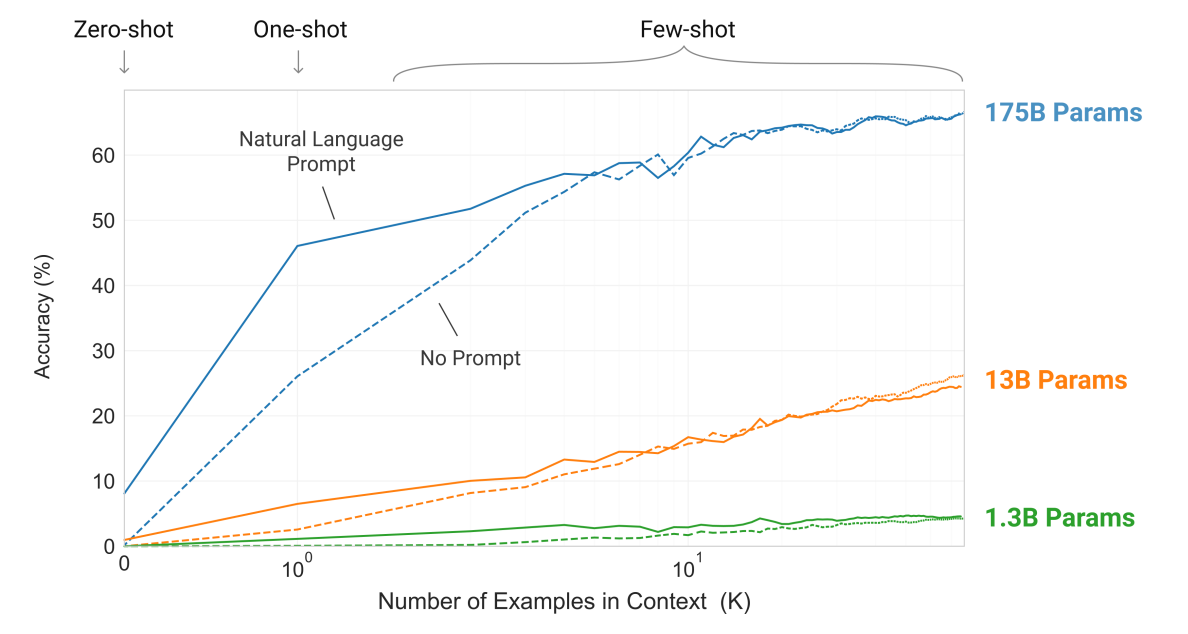
\includegraphics[width=0.7\textwidth]{graphics/fewshot.png}
  \caption[Zero-Shot und Few-Shot Prompting im Vergleich]{Zero-Shot und Few-Shot Prompting im Vergleich\footcite[Entnommen aus][]{brown2020gpt3fewshot}}
  \label{fig:fewshot}
\end{figure}


\subsection{\acs{RAG} und Fine-Tuning als Erweiterungsansätze}

\textbf{\acf{RAG}} erweitert den Prompt zur Laufzeit mit thematisch passenden Dokumenten aus einer externen Wissensbasis und könnte im Accessibility-Kontext aktuelle \ac{WCAG}-Kriterien unabhängig vom Trainings-Cutoff abrufbar machen.\footcite[Vgl.][S. 1--2]{lewisRetrievalAugmentedGenerationKnowledgeIntensive2021} \textbf{Fine-Tuning} bezeichnet das domänenspezifische Training auf einem aufgabenspezifischen Datensatz; für den Kontext der \ac{BITBW} wäre insbesondere ein Fine-Tuning auf \ac{BITV}-spezifischen Anforderungen denkbar.\footcite[Vgl.][S. 90]{silvestreSystemsOpportunitiesLLM2025} Beide Ansätze liegen außerhalb des Scopes dieser Arbeit und werden im Ausblick (Abschnitt~\ref{sec:fazit_ausblick}) aufgegriffen.

\subsection{Datenschutz bei \ac{KI}-gestützten Accessibility-Services} \label{datenschutz}

Der Einsatz von \ac{LLM}s im Kontext öffentlicher Verwaltungen wirft spezifische Datenschutzfragen auf. Webanwendungen der öffentlichen Verwaltung verarbeiten häufig personenbezogene Daten -- etwa in Formularseiten, die persönliche Angaben von Bürgerinnen und Bürgern erfassen. Werden diese Seiten für eine \ac{KI}-gestützte Accessibility-Analyse an externe \ac{LLM}-\ac{API}s übermittelt, ist die Wahrung der Datenschutzgarantien fraglich.

Die \ac{DSGVO} schreibt vor, dass personenbezogene Daten nur auf Basis einer Rechtsgrundlage und unter Wahrung der Grundsätze der Zweckbindung und Datenminimierung verarbeitet werden dürfen.\footcite[Vgl.][]{dsgvo2016} Die Übermittlung von \ac{HTML}-Quellcode der produktiven Anwendung, der im schlimmsten Fall personenbezogene Daten als Attributwerte enthalten kann, an externe \ac{API}-Dienste wie die OpenAI \ac{API} oder die Anthropic \ac{API} ist ohne explizite Rechtsgrundlage und einen Auftragsverarbeitungsvertrag nach Art. 28 \ac{DSGVO} für öffentliche Verwaltungen in Deutschland problematisch.\footcite[Vgl.][Art. 28]{dsgvo2016}

Als Lösungsansatz wird in dieser Arbeit ein Lokal-First-Prinzip verfolgt: Das \ac{KI}-Assistenzsystem soll ohne externe \ac{API}-Aufrufe betreibbar sein, indem lokal ausführbare Open-Source-Modelle -- etwa Modelle der LLaMA-Familie oder Mistral -- eingesetzt werden.\footcite[Vgl.][]{touvron2023llama2} Damit bleiben sämtliche Analyse- und Codedaten innerhalb der eigenen Infrastruktur. Diese Anforderung prägt sowohl die nicht-funktionalen Anforderungen (Kapitel \ref{kap:4}) als auch die Architekturentscheidungen (Kapitel \ref{kap:6}) dieser Arbeit.

Die in diesem Kapitel erarbeiteten theoretischen Grundlagen -- das normative Fundament der \ac{WCAG}, die empirisch belegten Grenzen regelbasierter Tools, die Besonderheiten von React-Anwendungen sowie die Möglichkeiten und Grenzen von \ac{LLM}s und des Prompt Engineerings -- bilden den konzeptionellen Rahmen für die im folgenden Kapitel aufgearbeitete Forschungsliteratur sowie für die anschließend dargestellte Methodik.
\chapter{Stand der Forschung} \label{kap:3}

Das folgende Kapitel gibt einen thematisch strukturierten Überblick über den Forschungsstand zur \ac{KI}-gestützten Barrierefreiheitsanalyse. Darauf aufbauend werden die verbleibenden Forschungslücken herausgearbeitet, die den Ausgangspunkt der vorliegenden Arbeit bilden. Die relevanten Arbeiten lassen sich drei Entwicklungslinien zuordnen: (1) \ac{LLM}-basierte Erkennung von Accessibility-Verstößen, (2) \ac{LLM}-basierte Korrektur und Code-Generierung sowie (3) hybride Pipelines, die regelbasierte Tools mit \ac{LLM}-Analyse kombinieren.

\section{Vorgehen der Literaturrecherche}

Zur Einordnung des Forschungsstands wurde eine strukturierte Literaturrecherche in wissenschaftlichen Datenbanken durchgeführt (ACM Digital Library, IEEE Xplore, ScienceDirect, arXiv, ResearchGate).\footcite[Vgl.][]{WebsterWatson2002} Die Recherche erfolgte themenorientiert auf Basis von Suchbegriffen wie \glqq web accessibility\grqq, \glqq LLM accessibility\grqq, \glqq accessibility violation detection\grqq{} und \glqq axe-core\grqq; berücksichtigt wurden primär aktuelle Arbeiten mit Bezug zur automatisierten Erkennung oder Behebung von Barrierefreiheitsverstößen in Webanwendungen mit \ac{KI}-Assistenzsystemen. Die identifizierten Arbeiten wurden thematisch gruppiert, priorisiert und vergleichend ausgewertet.

\section{Von frühen \acs{KI}-Ansätzen zur \acs{LLM}-basierten Erkennung}

Delnevo et al. (2024) zeigen, dass GPT-3.5 einfache syntaktische Verstöße mit moderater Genauigkeit erkennt, bei semantischen Problemen jedoch inkonsistente Bewertungen liefert.\footcite[Vgl.][]{delnevo_interaction_2024} Bassi et al. (2025) vergleichen GPT-4o, GPT-3.5 und LLaMA~3.1 in einer zweistufigen Evaluation; GPT-4o identifiziert 74\% der Verstöße korrekt, während 15\% als Halluzinationen eingestuft werden.\footcite[Vgl.][S. 302]{bassi_assessment_2025} Eine nachgelagerte Chain-of-Verification-Stufe erhöht die Zuverlässigkeit deutlich; \ac{RAG} wird nur als zukünftige Erweiterung diskutiert.\footcite[Vgl.][S. 301]{bassi_assessment_2025}

\section{\acs{LLM}-basierte Korrektur und Prompt-Engineering}

Abu Doush und Kassem (2024) zeigen, dass strukturierte Prompts die Qualität \ac{LLM}-generierter barrierefreier \acs{HTML}-Alternativen erheblich verbessern, bei komplexen Interaktionsmustern aber weiterhin Schwächen bestehen.\footcite[Vgl.][S. 343]{doush_evaluating_2025} Guriță und Vatavu (2025) belegen, dass accessibility-orientierte Prompts paradoxerweise mehr Violations erzeugen können als neutrale -- erst iteratives Prompting über fünf Runden senkte den Violation Score von 0,84 auf 0,32.\footcite[Vgl.][S. 1000]{gurita_insights_2025}

Den aktuellen Stand der Technik repräsentiert \textfett{AccessGuru} von Fathallah et al. (2025).\footcite[Vgl.][]{fathallah_accessguru_2025} Das System kombiniert eine zweistufige Pipeline -- zunächst regelbasierte Detection via Playwright und \textfett{axe-core}, anschließend eine \ac{LLM}-basierte Korrektur durch GPT-4o mit Role-Play, Contextual und Metacognitive Prompting. Corrective Re-Prompting verbessert den Violation Score Decrease von 0,72 auf 0,84 bei einer semantischen Ähnlichkeit von 77\% zu menschlichen Referenzlösungen. Als offenes Problem benennen die Autoren die fehlende Verknüpfung korrigierter \acs{HTML}-Snippets mit dem Quellcode der geprüften Anwendung.

Fernández-Navarro und Chicano (2026) erweitern diesen Ansatz um eine direkte Quellcode-Korrektur und adressieren damit explizit die Lücke zwischen \ac{DOM}-Korrektur und entwicklerseitiger Umsetzung.\footcite[Vgl.][]{fernándeznavarro2026automatedllmbasedaccessibilityremediation} Ihr Tool injiziert Korrekturen auf Basis einer Quellcodeanalyse gezielt in tatsächliche Komponentendateien und erreicht in der Evaluation über öffentliche Websites und Open-Source-Angular-Projekte Remediation Rates von über 80\% bei vollständiger Build-Integrität. Der Ansatz beschränkt sich jedoch auf Angular und setzt auf cloudbasiertes GPT-4o; eine Übertragung auf React wird von den Autoren als kurzfristiger Folgeschritt benannt.\footcite[Vgl.][]{fernándeznavarro2026automatedllmbasedaccessibilityremediation}

\section{Hybride Pipelines und Ensemble-Testing}

Huang et al. entwickeln 2024 mit \textfett{ACCESS} ein System, das Prompt-Engineering gezielt zur automatisierten Barrierefreiheitskorrektur einsetzt und dabei verschiedene Strategien systematisch vergleicht.\footcite[Vgl.][S. 7,9]{huang_access_2024} Der Vergleich von ReAct, Chain-of-Thought und Few-Shot Prompting zeigt, dass ReAct mit einem Severity Score Reduction von 51,3\% alle anderen Strategien übertrifft -- ein Ergebnis, das die Bedeutung iterativer, werkzeuggestützter Reasoning-Strategien für diese Aufgabe unterstreicht.

He et al. präsentieren 2025 mit \textfett{GenA11y} das methodisch ausgefeilteste Detection-System des aktuellen Forschungsstands.\footcite[Vgl.][FSE101:20--21]{he_enhancing_2025} \textfett{GenA11y} extrahiert nach vollständigem clientseitigem Rendering den \ac{DOM} via Playwright und prüft ihn anschließend kriteriumsspezifisch mit GPT-4o. Eine Ablation Study belegt, dass weder \ac{DOM}-Extraktion noch optimiertes Prompting allein die Gesamtleistung von Precision 94,5\% und Recall 87,61\% erreichen.\footcite[Vgl.][FSE101:20]{he_enhancing_2025} \textfett{GenA11y} erkennt acht Verstoßtypen, die von keinem der verglichenen regelbasierten Tools gefunden werden.\footcite[Vgl.][FSE101:20]{he_enhancing_2025} Paternò et al. ergänzen dieses Bild mit \textfett{TeVal}, das semantische \ac{WCAG}-Kriterien durch Role-Play Prompting mit Few-Shot-Beispielen und Confidence Score bewertet und dabei eine Effektivität von 92,4\% erzielt.\footcite[Vgl.][]{paterno_how_2025}

Pool (2023) adressiert die Detection-Schicht mit \textfett{Testaro}, einem Ensemble aus acht Accessibility-Werkzeugen (u.\,a. axe-core, WAVE, QualWeb); die Analyse zeigt, dass jedes Tool exklusive Violations erkennt und die Werkzeuge damit komplementär wirken.\footcite[Vgl.][]{pool_testaro_2023}

\section{Forschungslücken und Einordnung der vorliegenden Arbeit} \label{Forschungslücken}

Die Analyse der bestehenden Forschungsarbeiten zeigt drei persistente Forschungslücken, die den Ausgangspunkt der vorliegenden Arbeit definieren.

Erstens berücksichtigt keiner der untersuchten Ansätze systematisch zustandsabhängige Barrieren, die erst durch Nutzerinteraktionen in React-basierten Single-Page Applications entstehen.\footcite[Vgl.][S. 110]{tafreshipour_ma11y_2024} Zwar setzen einzelne Systeme wie \textfett{AccessGuru} Playwright zur \ac{DOM}-Extraktion ein, jedoch beschränkt sich dies auf das initiale Rendering -- interaktionsbedingte Zustandswechsel werden nicht geprüft.\footcite[Vgl.][]{fathallah_accessguru_2025}

Zweitens verknüpft kein bekannter Ansatz Tool-Reports mit dem Quellcode der geprüften Anwendung. \textfett{AccessGuru} selbst benennt dies als offenes Problem: die generierten Korrekturen beziehen sich auf isolierte \ac{DOM}-Snippets und nicht auf die \ac{JSX}-Komponenten, in denen Entwicklerinnen und Entwickler tatsächlich eingreifen müssten.\footcite[Vgl.][]{fathallah_accessguru_2025} Die Lücke zwischen technischer Fehlererkennung und entwicklernaher Umsetzung bleibt damit bestehen.

Drittens adressiert keine der untersuchten Arbeiten die datenschutzrechtlichen Anforderungen öffentlicher Verwaltungen: alle Systeme setzen auf cloudbasierte \ac{LLM}-\ac{API}s (primär GPT-4o), was für die \ac{BITBW} und vergleichbare Institutionen ohne vertiefte datenschutzrechtliche Prüfung nicht nutzbar ist.\footcite[Vgl.][Art. 28, 44 ff.]{dsgvo2016}

Die Konzeptmatrix in Tabelle \ref{tab:konzeptmatrix_haupt} fasst die zentralen Merkmale der untersuchten Studien im Vergleich zum eigenen \ac{PoC} zusammen und macht die identifizierten Forschungslücken strukturell sichtbar.

\newcolumntype{A}{>{\raggedright\arraybackslash}p{4.3cm}} % Autor/Jahr
\newcolumntype{S}{>{\raggedright\arraybackslash}p{2.8cm}} % System
\newcolumntype{C}{>{\centering\arraybackslash}p{0.55cm}}  % Konzept-Spalten (alle gleich breit)

\newcommand{\lhdr}[2]{\parbox[c][32mm][c]{#1}{\centering\textbf{#2}}}
\newcommand{\hdr}[1]{\rotatebox{90}{\scriptsize\strut #1}}

\newcommand{\yes}{\textbf{x}}

\begin{table}[htbp]
\centering
\setlength{\tabcolsep}{2.5pt}
\renewcommand{\arraystretch}{1.25}

\resizebox{\textwidth}{!}{%
\begin{tabular}{|A|S||*{14}{C|}}
\hline
\multicolumn{2}{|c||}{\textbf{Studie}} &
\multicolumn{14}{c|}{\textbf{Konzepte}} \\
\hline

\multirow{2}{*}{\lhdr{4.3cm}{Autor(en)\\\& Jahr}} &
\multirow{2}{*}{\lhdr{2.8cm}{System}} &
\multicolumn{3}{c|}{\textbf{Ziel}} &
\multicolumn{3}{c|}{\textbf{Datenquellen}} &
\multicolumn{3}{c|}{\textbf{\ac{KI}-/\ac{LLM}-Ansatz}} &
\multicolumn{3}{c|}{\textbf{Evaluation}} &
\multicolumn{2}{c|}{\textbf{Kontext}} \\
\cline{3-16}

& &
\hdr{\ac{WCAG}-Konf.\ prüfen} &
\hdr{Barrieren korrigieren} &
\hdr{Entwickler unterstützen} &
\hdr{Tool-Reports (axe etc.)} &
\hdr{Interaktionsdaten (Playwright)} &
\hdr{Quellcode-Analyse} &
\hdr{\ac{LLM}-basiert} &
\hdr{Kontextsensitiv / \ac{RAG}} &
\hdr{Lokal ausführbar} &
\hdr{Automatisierte Eval.} &
\hdr{Qualitative Eval.} &
\hdr{Nutzerstudie} &
\hdr{Rich-Client / \ac{SPA}} &
\hdr{Rechtl.\ Rahmen (\ac{BFSG} etc.)} \\
\hline

% ── HOCH-priorisierte Studien ────────────────────────────────
\multicolumn{16}{|l|}{\textbf{Hoch priorisierte Studien}} \\
\hline

He et al.\ (2025) & GenA11y
& \yes &   &   & \yes &   &   & \yes &   &   & \yes &   &   &   &   \\ \hline

Fathallah et al.\ (2025) & AccessGuru
& \yes & \yes & \yes & \yes & \yes &   & \yes &   &   & \yes &   &   &   &   \\ \hline

Bassi et al.\ (2025) & \ac{LLM} Auditing
& \yes & \yes & \yes &   &   &   & \yes &   &   &   & \yes &   &   & \yes \\ \hline

Paternò et al.\ (2025) & TeVal
& \yes &   & \yes & \yes &   &   & \yes & \yes &   &   & \yes &   &   &   \\ \hline

Tafreshipour et al.\ (2024) & Ma11y
& \yes &   &   & \yes & \yes &   &   &   &   & \yes &   &   &   &   \\ \hline

Fernández-Navarro \& Chicano (2026) & \ac{LLM} Remediation
& \yes & \yes & \yes & \yes &   & \yes & \yes &   &   & \yes &   &   & \yes &   \\ \hline

% ── Eigener PoC ──────────────────────────────────────────────

\textbf{Martinez Campo (2026)} &
\textbf{ACE (\ac{PoC})}
& \yes & \yes & \yes
& \yes & \yes & \yes
& \yes & \yes & \yes
&   & \yes &
& \yes & \yes \\ \hline

\end{tabular}%
}% Ende resizebox

\caption[Konzeptmatrix (Hauptmatrix, hoch priorisierte Studien)]{%
  Konzeptmatrix nach Webster Watson\footnotemark: hoch priorisierte Studien im Vergleich
  zum eigenen \acf{PoC}. \yes~=~Konzept vorhanden/adressiert; leer ~=~nicht adressiert.
  Für den eigenen \ac{PoC} bezeichnen die Markierungen angestrebte Designziele, deren Umsetzung und Wirksamkeit in Kapitel~\ref{kap:7} evaluiert wird.
  Die vollständige Matrix aller analysierten Studien findet sich in Anhang~\ref{app:konzeptmatrix}.}
\label{tab:konzeptmatrix_haupt}
\end{table}
\footnotetext{Vgl. \cite{WebsterWatson2002}.}

\chapter{Methodik} \label{kap:methodik}

Das folgende Kapitel beschreibt das methodische Vorgehen der Arbeit. Zunächst wird die gewählte Forschungsmethode begründet (Abschnitt~\ref{sec:wiss_methode}), anschließend der Untersuchungsgegenstand abgegrenzt (Abschnitt~\ref{sec:scope}) und schließlich das Evaluationsdesign mit den zugehörigen Bewertungskriterien definiert (Abschnitt~\ref{sec:eval}).

\section{Wissenschaftliche Methode} \label{sec:wiss_methode}

Die vorliegende Arbeit folgt dem Forschungsparadigma des \ac{DSR}, das von Hevner et al. für die Wirtschaftsinformatik systematisiert wurde.\footcite[Vgl.][]{hevner2004dsr} \ac{DSR} eignet sich für diese Arbeit aus zwei Gründen: Erstens steht die Konstruktion eines konkreten technischen Artefakts im Zentrum der Forschungsfrage, nicht die Überprüfung einer statistischen Hypothese. Zweitens fordert \ac{DSR} explizit die Evaluation des Artefakts in einem realen Anwendungskontext, was dem praxisorientierten Charakter der Arbeit entspricht.\footcite[Vgl.][S. 80]{hevner2004dsr}

Alternative Ansätze wie Action Research oder kontrollierte Experimente wurden verworfen: Action Research setzt eine mehrjährige Praktikerzusammenarbeit voraus; kontrollierte Experimente erfordern eine Stichprobenbasis, die im Verwaltungskontext nicht verfügbar ist.\footcites[Vgl.][S. 1--2]{baskerville1999ar}[Vgl.][S. 239--335]{baskerville2004ar}

Als prozessualer Rahmen dient das sechsphasige DSRM-Prozessmodell nach Peffers et al.\footcite[Vgl.][]{peffers2007dsrm} Die Zuordnung der einzelnen Phasen zu den Kapiteln dieser Arbeit zeigt Tabelle~\ref{tab:dsrm_mapping}.

\begin{table}[htbp]
\centering
\begin{tabular}{|l|l|}
\hline
\textbf{DSRM-Phase} & \textbf{Kapitel} \\
\hline
Problem-Identifikation & Kapitel \ref{kap:1}-\ref{kap:3} \\
Zieldefinition & Kapitel \ref{kap:1.3} \& \ref{Forschungslücken} \\
Design \& Entwicklung & Kapitel \ref{kap:4}-\ref{kap:6} \\
Demonstration & Kapitel \ref{kap:6} (insb. Beispielabläufe) \\
Evaluation & Kapitel \ref{kap:7} \\
Kommunikation & Gesamtarbeit, zusammenfassend Kapitel \ref{kap:8} \\
\hline
\end{tabular}
\caption{Zuordnung der DSRM-Phasen zu den Kapiteln der Arbeit.}
\label{tab:dsrm_mapping}
\end{table}

Ergänzt wird dieser Rahmen durch einen Fallstudienansatz nach Yin.\footcite[Vgl.][]{yin_case_2018} Der \ac{BWEC} dient als Einzelfallstudie, da die Forschungsfrage auf ein zeitgenössisches Phänomen in einem spezifischen Praxiskontext abzielt, bei dem die Grenzen zwischen technischem System und organisatorischem Kontext nicht trennscharf sind.

Die Wahl eines \ac{PoC} als Artefakttyp ist durch die explorative Natur der Forschungsfrage begründet: Das Ziel ist die konzeptionelle Demonstration der technischen Machbarkeit, nicht die statistisch belastbare Generalisierung auf eine Grundgesamtheit.\footcite[Vgl.][]{hevner2004dsr}

\section{Untersuchungsgegenstand und Scope-Abgrenzung} \label{sec:scope}

Als Praxisrahmen und Motivationskontext dient der \ac{BWEC}, eine öffentlich zugängliche React-basierte Webanwendung der \ac{BITBW}.\footcite[Vgl.][]{bwec} Er vereint drei für die Forschungsfrage zentrale Merkmale: gesetzlich relevante Anforderungen an digitale Barrierefreiheit, einen datenschutzsensiblen Einsatzkontext in der öffentlichen Verwaltung sowie typische Interaktionsmuster moderner Single-Page Applications. Die formale Hauptevaluation erfolgt hingegen an synthetisch konstruierten Testsuiten (test-12, test-50, test-100) mit vollständig bekannter Ground Truth. Der \ac{BWEC} wird ergänzend als Feldtest ohne quantitativen Ground-Truth-Vergleich eingesetzt (vgl. Abschnitt~\ref{sec:eval_bwec}).

Der Untersuchungsscope ist wie folgt abgegrenzt:

\begin{itemize}
    \item \textbf{Eingeschlossen:} Öffentlich zugängliche Bereiche der Anwendung ohne Authentifizierung. Betrachtet werden \ac{WCAG}~2.2-Verstöße auf Konformitätsstufe A und AA, soweit sie durch regelbasierte Prüfung, \ac{DOM}-Analyse und Interaktionsausführung im Frontend beobachtbar sind.\footcite[Vgl.][]{WCAG}
    \item \textbf{Ausgeschlossen:} Backend-Logik, Datenbankstrukturen sowie eine vollständige rechtliche Bewertung im Sinne einer formalen \ac{BITV}-Prüfung.\footcite[Vgl.][]{BITV}
\end{itemize}

Die Einschränkungen hinsichtlich vollständiger \ac{WCAG}-Abdeckung und Generalisierbarkeit auf beliebige Frameworks werden in Kapitel~\ref{kap:7} als Limitationen diskutiert.

\section{Evaluationsdesign und Kriterien} \label{sec:eval}

Ziel der Evaluation ist es, die technische Machbarkeit und den praktischen Nutzen des entwickelten \ac{PoC} anhand synthetisch konstruierter Testsuiten mit vollständig bekannter Ground Truth zu untersuchen. Der \ac{BWEC} dient ergänzend als Feldtest-Kontext ohne quantitativen Recall-Vergleich (vgl. Abschnitt~\ref{sec:eval_bwec}).

\subsection{Evaluationslogik}

Die Evaluation folgt einem fünfstufigen Vorgehen:

\begin{enumerate}
    \item \textbf{Testsuite-Konstruktion:} Drei synthetische React-\acp{SPA} werden mit gezielt eingebetteten \ac{WCAG}-Violations entwickelt (test-12: 12, test-50: 50, test-100: 100~Violations), die alle drei Verstoßkategorien der in Abschnitt~\ref{Taxonomie} eingeführten Taxonomie abdecken.\footcite[Vgl.][]{WCAG}
    \item \textbf{Benchmarkläufe:} Jede Suite wird mit drei Modellen je zehn Mal analysiert (insgesamt 90~Runs). Pro Lauf werden Recall, Priorisierungsverhalten, Fix-Qualität und Laufzeit erfasst.
    \item \textbf{Recall-Auswertung:} Die Ergebnisse werden mit der bekannten Ground Truth verglichen. Eine Violation gilt als erkannt, wenn sie in der Mehrzahl der zehn Runs im finalen \ac{LLM}-Report erscheint.
    \item \textbf{Qualitative Empfehlungsbewertung:} Die generierten Handlungsempfehlungen werden anhand einer dreistufigen Bewertungsskala (Stufe~0--2) nach Dateikonkretheit und Code-Fix-Qualität bewertet.
    \item \textbf{\ac{BWEC}-Feldtest:} Die Pipeline wird ergänzend auf dem realen \ac{BWEC}-Untersuchungsobjekt eingesetzt, um Systemstabilität und qualitative Plausibilität unter realen Bedingungen zu prüfen.\footcites[Vgl.][]{axe}[Vgl.][]{kodithuwakku_assessing_2025}
\end{enumerate}

\subsection{Bewertungskriterien}

Die Evaluation erfolgt anhand von vier Kriterien, die auf Basis der Forschungsfragen und der Fachliteratur entwickelt wurden.

\textbf{Kriterium 1 -- Korrektheit der Erkennung:} Die vom System identifizierten Verstöße werden mit der bekannten Ground Truth der synthetischen Testsuiten verglichen. Als Orientierungswerte dienen die Ergebnisse vergleichbarer Systeme: \textfett{GenA11y} erreicht eine Precision von 94,5\% und einen Recall von 87,61\%.\footcite[Vgl.][FSE101:20]{he_enhancing_2025}

\textbf{Kriterium 2 -- Qualität der Handlungsempfehlungen:} Die generierten Empfehlungen werden anhand einer dreistufigen Skala (Stufe~0--2) qualitativ bewertet: Stufe~2 bezeichnet einen konkreten Fix mit Dateiname, Zeilennummer und umsetzbarem Code-Vorschlag; Stufe~1 einen zutreffenden Fix-Typ ohne Quellcode-Kontext; Stufe~0 eine generische Problembeschreibung. \textfett{AccessGuru} erreicht als Referenzwert einen Violation Score Decrease von 84\%.\footcite[Vgl.][]{fathallah_accessguru_2025}

\textbf{Kriterium 3 -- Mehrwert der Kontextualisierung:} Der Zusatznutzen der vollständigen Kontextkombination wird durch einen systematischen Vergleich zweier Konfigurationen ermittelt: (a)~die reine Tool-Baseline (axe-core, Playwright, grep ohne \ac{LLM}-Kontextualisierung) und (b)~die vollständige Pipeline (Baseline + \ac{LLM}-gestützte Quellcodeanalyse). Verglichen werden Recall, Fix-Qualität sowie die Fähigkeit, datei- und zeilenspezifische Handlungsempfehlungen zu generieren.\footnote{Siehe Abschnitt~\ref{kap:1.3}.}

\textbf{Kriterium 4 -- Technische Praktikabilität:} Laufzeit, Stabilität und Qualität des \acs{JSON}-Outputs werden unter realen Bedingungen dokumentiert.

\subsection{Limitationen des Evaluationsdesigns}

Zwei methodische Einschränkungen sind vorab zu benennen. Erstens wird die Bewertung durch den Autor selbst durchgeführt und nicht durch unabhängige Gutachter validiert. Zweitens sind die genannten Referenzwerte von \textfett{AccessGuru}\footcite[Vgl.][]{fathallah_accessguru_2025} und \textfett{GenA11y}\footcite[Vgl.][]{he_enhancing_2025} nur eingeschränkt vergleichbar, da sie auf anderen Datensätzen und unter anderen Rahmenbedingungen ermittelt wurden. Sie dienen daher als Orientierung, nicht als direkter Benchmark.
\chapter{Analyse und Anforderungen}\label{kap:4}

Dieses Kapitel erarbeitet die Grundlagen für das in Kapitel~\ref{kap:5} beschriebene Systemdesign. Zunächst werden Problemkontext und Handlungsbedarf analysiert. Anschließend werden die funktionalen und nicht-funktionalen Anforderungen an das zu entwickelnde System spezifiziert. Abschließend wird die Auswahl der eingesetzten Inferenzinfrastruktur und der Modellkandidaten begründet.

\section{Problemkontext und Handlungsbedarf}\label{kap:4.1}

Wie in Kapitel~\ref{kap:1} dargelegt, unterliegen alle von der \ac{BITBW} entwickelten und betriebenen Web\-anwendungen den gesetzlichen Anforderungen der \ac{BITV} 2.0, für die \ac{WCAG} 2.2 auf Konformitätsstufe AA den verbindlichen Maßstab bildet.\footcites[Vgl.][S. 475]{heinemann_barrierefreiheit_2024}[][]{BITV} In der Praxis erfolgt die Barrierefreiheitsprüfung bislang überwiegend manuell oder mithilfe einzelner regelbasierter Tools. Dieses Vorgehen ist aus zwei Gründen problematisch: Manuelle Audits sind personalintensiv und skalieren nur unzureichend mit der Anzahl zu betreuender Anwendungen; regelbasierte Tools erfassen, wie in Kapitel~\ref{tools} dargelegt, nur einen Bruchteil der tatsächlich vorhandenen Barrieren.\footcite[Vgl.][S. 8--9]{tafreshipour_ma11y_2024}

Die in Kapitel~\ref{kap:3} identifizierten drei Forschungslücken bilden den Ausgangspunkt der Anforderungserhebung.\footcites[Vgl.][S. 9--11, 23--24]{hevnerChatterjeeDesignResearch2010} Dazu zählen die fehlende Zustandserfassung durch Interaktionen, die fehlende Verknüpfung von \ac{DOM}-Befunden mit dem Quellcode sowie die Anforderungen an digitale Souveränität und den Datenschutzvorgaben öffentlicher Verwaltungen, die den Einsatz cloudbasierter \ac{LLM}-\ac{API}s ausschließen (vgl. Abschnitt~\ref{datenschutz}). Daraus ergibt sich als Systemziel ein lokal ausführbares, \ac{LLM}-gestütztes Assistenzsystem, das axe-core-Reports, Playwright-Interaktionsdaten und statische Quellcodeanalyse kombiniert (vgl. Abschnitt~\ref{kap:1.3}).

\section{\acl{FA}} \label{kap:4.2}

\acf{FA} beschreiben die Leistungen, die ein System erbringen soll.\footcite[Vgl.][S. 105--107]{sommerville2016software} Die folgenden Anforderungen leiten sich aus der Problemanalyse (Abschnitt~\ref{kap:4.1}), den identifizierten Forschungslücken (Abschnitt~\ref{Forschungslücken}) sowie der Analyse vergleichbarer Systeme \mbox{aus der Literatur ab}.

\clearpage
\textfett{\acs{FA}-01 Regelbasierte Accessibility-Erkennung}

Das System muss den \ac{BWEC} automatisiert auf Barrierefreiheitsverstöße gemäß \ac{WCAG} 2.2 der Konformitätsstufen A und AA prüfen.\footcite[Vgl.][]{bwec,WCAG} Die Prüfung basiert auf axe-core als Detection-Backend.\footcite[Vgl.][]{axe} Der Output je Verstoß umfasst mindestens: Regel-ID, Schweregrad (critical/serious/moderate/minor) sowie ein \acs{HTML}-Ausschnitt des betroffenen Elements.

\textfett{\acs{FA}-02 Dynamische Zustandserfassung via Playwright}

Das System muss mit Playwright definierte Interaktionssequenzen ausführen und zustandsabhängige Barrieren durch generische Interaktionschecks erfassen.\footcite[Vgl.][]{playwright} Damit werden Barrieren erfasst, die im initialen Seitenzustand nicht vorhanden sind.\footnote{Siehe Kapitel \ref{Herausforderungen}}

\textfett{\acs{FA}-03 Statische Quellcodeanalyse}

Das System muss den Quellcode der geprüften React-Anwendung automatisiert auf Muster untersuchen, die auf Barrierefreiheitsprobleme hindeuten, etwa fehlende \texttt{aria}-Attribute, \texttt{onClick}-Handler auf nicht-interaktiven Elementen, fehlende \texttt{alt}-Attribute sowie fehlende Formular-Assoziationen.\footnote{Siehe Kapitel \ref{kap:2.1}}

\textfett{\ac{FA}-04 \ac{LLM}-gestützte Analyse und Handlungsempfehlung}

Das System muss die Ergebnisse aus \ac{FA}-01, \ac{FA}-02 und \ac{FA}-03 in einem strukturierten Kontext zusammenführen und an ein lokal ausgeführtes Sprachmodell übergeben, das daraus je Verstoß eine Handlungsempfehlung im Format Must-have/Nice-to-have unter Angabe der betroffenen Datei generiert.\footnote{Siehe Abschnitt~\ref{sec:kontextualisierung}}

\textfett{\ac{FA}-05 Strukturierter \acs{JSON}-Output}

Das System muss seine Ergebnisse in einem maschinenlesbaren \acs{JSON}-Format bereitstellen.\footcite[Vgl.][]{paterno_how_2025,pool_testaro_2023} Der Report enthält je Befund: Verstoß-ID, Kategorie (syntaktisch/semantisch/layout), Schweregrad, betroffene Datei(en), Handlungsempfehlung (Must-have/Nice-to-have), \ac{WCAG}-Erfolgskriterium und -- falls vorhanden -- den relevanten Quellcode-Ausschnitt.

\section{\acl{NFA}}\label{kap:4.3}

\acf{NFA} beschreiben die Qualitätseigenschaften des Systems. Für das vorliegende System haben sie besonderes Gewicht, da der Betriebskontext der \ac{BITBW} (öffentliche Verwaltung, lokale Infrastruktur) strenge Rahmenbedingungen setzt.

\textfett{\ac{NFA}-01 Digitale Souveränität und Lokal-First}

Das System muss vollständig ohne externe \ac{API}-Aufrufe betreibbar sein. Weder Quellcode noch \ac{DOM}-Inhalte noch Violation-Reports dürfen das interne Netzwerk verlassen. Dies folgt sowohl aus den Anforderungen an digitale Souveränität öffentlicher Verwaltungen als auch aus den datenschutzrechtlichen Vorgaben der \ac{DSGVO}.\footcites[Vgl.][]{bmds_digitale_souveraenitaet}[][Art. 28 und Art. 32]{dsgvo2016}

\textfett{\ac{NFA}-02 Laufzeit und Praktikabilität}

Der vollständige Analyselauf muss auf einem Entwicklungsrechner innerhalb einer für den Entwicklungsalltag praktikablen Zeit abgeschlossen werden. Als Richtwert gilt eine Gesamtlaufzeit von unter zehn Minuten für eine einzelne Seite mit bis zu 20 axe-Verstößen. Diese Anforderung schließt mehrstufige Reasoning-Schleifen aus dem Rahmen des \ac{PoC} aus.\footnote{Siehe Kapitel \ref{Prompt}}

\textfett{\ac{NFA}-03 Wartbarkeit und Erweiterbarkeit}

Die Systemarchitektur muss eine modulare Trennung der Komponenten (Detection, Context-Building, Synthesis) vorsehen, sodass einzelne Bestandteile unabhängig angepasst oder ausgetauscht werden können.

\textfett{\ac{NFA}-04 Reproduzierbarkeit}

Das System muss hinreichend deterministisch sein, damit zwei aufeinanderfolgende Analyseläufe auf derselben Anwendungsversion im Wesentlichen dieselben Befunde erzeugen. Reproduzierbarkeit wird durch eine feste Temperatur-Einstellung (\texttt{temperature} = 0.05) und durch strukturierte Ausgabeformate (\acs{JSON}-Schema im Prompt) sichergestellt.\footcites[Vgl.][Temperature]{OpenAI_Developers}[][Temperature]{anthropic2026claude}

\section{Lokale Inferenzinfrastruktur und Modellkandidaten}\label{kap:4.4}

Die Wahl der Inferenzinfrastruktur ist durch \ac{NFA}-01 (Lokal-First) weitgehend vorgegeben: Cloudbasierte Modell-\ac{API}s scheiden aus, da ihre Nutzung die Übermittlung potenziell schützenswerter Quellcodeausschnitte und \ac{DOM}-Inhalte an externe, überwiegend US-amerikanische Server erfordert -- was weder mit den Anforderungen an digitale Souveränität noch mit den datenschutzrechtlichen Vorgaben der \ac{DSGVO} vereinbar ist.\footcites[Vgl.][]{bmds_digitale_souveraenitaet}[][Art. 28 und Art. 44 ff.]{dsgvo2016}

\subsection{Ollama als Laufzeitumgebung}

Ollama ist ein quelloffenes Werkzeug, das die lokale Ausführung von \ac{LLM}s über eine einheit\-liche REST-\ac{API} ermöglicht.\footcite[Vgl.][]{Ollama} Die REST-\ac{API} ist kompatibel mit der OpenAI-\ac{API}-Spezifikation, wodurch sich bestehende Node.js-Bibliotheken ohne größeren Anpassungsaufwand integrieren lassen. Darüber hinaus unterstützt Ollama quantisierte Modellvarianten (z.\,B. Q4\_K\_M), die eine speichereffiziente Ausführung auf \ac{CPU}-basierten Systemen ohne dedizierte Grafikkarte ermöglichen. Dies ist insbesondere für Entwicklungsrechner der \ac{BITBW} relevant, bei denen nicht von \ac{GPU}-Hardware ausgegangen werden kann.

\subsection{Anforderungen an das Sprachmodell}

Unabhängig von der konkreten Modellwahl lassen sich vier zentrale Anforderungen an das Sprachmodell ableiten:\footcite[Vgl.][S. 3]{hui2024qwen25coder}

\begin{enumerate}
    \item \ac{JSX} und TypeScript verarbeiten können (\ac{FA}-03)
    \item Strukturierte Ausgaben in einem vorgegebenen Format erzeugen (\ac{FA}-05, \ac{NFA}-04)
    \item Innerhalb eines Kontextfensters von mindestens 8.192 Tokens arbeiten (\ac{FA}-04)
    \item Auf \ac{CPU}-basierten Systemen mit akzeptabler Latenz betreibbar sein, was die Modellgröße auf ca. 7--32 Milliarden Parameter begrenzt (\ac{NFA}-02)
\end{enumerate}

Die Auswahl konkreter Modellkandidaten sowie deren vergleichende Evaluation werden in Abschnitt~\ref{sec:kontextualisierung} bzw. Kapitel~\ref{kap:7} behandelt.

\subsection{Ausgewählte Modellkandidaten für die Evaluation}

Für die Evaluation in Kapitel~\ref{kap:7} werden vier lokal ausführbare Modellkandidaten betrachtet, soweit die verfügbaren Hardware-Ressourcen eine Ausführung zulassen: \texttt{qwen2.5-coder:7b}, \texttt{qwen2.5-coder:14b}\footcite[Vgl.][]{hui2024qwen25coder}, \texttt{qwen3:32b}\footcite[Vgl.][]{qwen3} und \texttt{deepseek-r1:70b}\footcite[Vgl.][]{deepseek}. Die Auswahl folgt dem Ziel, unterschiedliche Modellgrößen systematisch miteinander zu vergleichen: 7B und 14B repräsentieren ressourcenschonende Modelle für den operativen Lokalbetrieb, 32B einen mittleren Kompromiss aus Qualität und Laufzeit, 70B ein leistungsstarkes Referenzmodell mit höherem Rechenbedarf. DeepSeek-R1:70b wurde als Kandidat betrachtet, konnte jedoch aufgrund der verfügbaren Hardware-Ressourcen und der damit verbundenen Laufzeitanforderungen nicht in die finale Benchmarkserie aufgenommen werden; die Evaluation in Kapitel~\ref{kap:7} basiert daher auf den drei verbleibenden Modellen.

\subsection{Zusammenfassung der Anforderungen}

Tabelle~\ref{tab:anforderungen} fasst die spezifizierten Anforderungen zusammen und ordnet ihnen jeweils Ursprung und Priorität zu.

\begin{table}[tp]
\centering
\footnotesize
\renewcommand{\arraystretch}{1.2}

\resizebox{\textwidth}{!}{%
\begin{tabular}{|l|p{5.5cm}|p{4.5cm}|l|}
\hline
\textbf{ID} & \textbf{Beschreibung} & \textbf{Ursprung} & \textbf{Priorität} \\
\hline
\multicolumn{4}{|l|}{\textbf{Funktionale Anforderungen}} \\
\hline
\ac{FA}-01 & Regelbasierte Accessibility-Erkennung via axe-core & Forschungsliteratur (Kap.~\ref{kap:3}) & Muss \\
\hline
\ac{FA}-02 & Dynamische Zustandserfassung via Playwright & Forschungslücke~1 (Kap.~\ref{Forschungslücken}) & Muss \\
\hline
\ac{FA}-03 & Statische Quellcodeanalyse (grep-basiert) & Forschungslücke~2 (Kap.~\ref{Forschungslücken}) & Muss \\
\hline
\ac{FA}-04 & \ac{LLM}-gestützte Analyse und Handlungsempfehlung & Forschungsliteratur (Kap.~\ref{kap:3}) & Muss \\
\hline
\ac{FA}-05 & Strukturierter \acs{JSON}-Output & Praxisanforderung \ac{BITBW} & Muss \\
\hline
\multicolumn{4}{|l|}{\textbf{Nicht-funktionale Anforderungen}} \\
\hline
\ac{NFA}-01 & Digitale Souveränität und Lokal-First (kein externer \ac{API}-Aufruf) & Institutionell (Dig. Souveränität, \ac{DSGVO}, \ac{BITBW}) & Muss \\
\hline
\ac{NFA}-02 & Laufzeit $<$\,10\,min pro Seite (ohne \ac{GPU}) & Praxisanforderung \ac{BITBW} & Soll \\
\hline
\ac{NFA}-03 & Wartbarkeit und Erweiterbarkeit (modulare Architektur) & Software-Engineering Best Practice & Soll \\
\hline
\ac{NFA}-04 & Reproduzierbarkeit (Temperature\,=\,0.05, \acs{JSON}-Schema) & Forschungsmethodik & Soll \\
\hline
\end{tabular}%
}

\caption[Anforderungsübersicht: funktionale und nicht-funktionale Anforderungen]{Anforderungsübersicht: funktionale und nicht-funktionale Anforderungen mit Ursprung und Priorität.}
\label{tab:anforderungen}
\end{table}

Die Anforderungen \ac{FA}-01 bis \ac{FA}-05 sowie \ac{NFA}-01 bis \ac{NFA}-04 bilden die verbindliche Grundlage für das Systemdesign in Kapitel~\ref{kap:5}. \ac{NFA}-01 (Lokal-First) hat dabei Vorrang vor allen anderen Anforderungen und schränkt den Lösungsraum strukturell ein.
\chapter{Konzeption des Assistenzsystems}
\label{chap:konzeption}

Das vorliegende Kapitel beschreibt die konzeptionelle Grundlage des entwickelten Assistenzsystems. 
Ausgehend von den in Kapitel~4 ermittelten Anforderungen werden zunächst die Zielarchitektur 
und die Datenpipeline erläutert, bevor das Modell der Kontextualisierung und Priorisierung sowie 
das gewählte Ausgabeformat vorgestellt werden. Jede Entwurfsentscheidung wird dabei mit 
Bezug auf die identifizierten funktionalen und nicht-funktionalen Anforderungen begründet.

% ─────────────────────────────────────────────────────────────────────────────
\section{Zielarchitektur und Datenpipeline}
\label{sec:zielarchitektur}

Die Zielarchitektur des Systems folgt dem Prinzip einer sequenziellen Datenpipeline, 
die drei voneinander unabhängige Analysequellen zusammenführt und deren Ergebnisse 
in einem einheitlichen Schema normalisiert, bevor sie an ein lokales Sprachmodell 
übergeben werden. Abbildung~\ref{fig:pipeline} illustriert den Gesamtablauf.

% TODO: Abbildung der Pipeline hier einfügen
% \begin{figure}[h]
%   \centering
%   \includegraphics[width=\textwidth]{figures/pipeline.pdf}
%   \caption{Datenpipeline des ACE-Assistenzsystems}
%   \label{fig:pipeline}
% \end{figure}

Die Pipeline gliedert sich in vier Phasen: die parallele Datenerhebung durch axe-core, 
Playwright und grep, die Normalisierung der Rohdaten in das Unified Finding Schema (UFS), 
die Prompt-Konstruktion mit Token-Budget-Steuerung sowie die Inferenz durch das lokale 
Sprachmodell und die anschließende Ausgabe.

\subsection{Analysequellen}

Das System nutzt drei komplementäre Werkzeuge zur Datenerhebung, die jeweils 
unterschiedliche Aspekte der Barrierefreiheit abdecken und sich gegenseitig ergänzen.

\textbf{axe-core} wird über einen gesteuerten Chromium-Browser ausgeführt und analysiert 
den vollständig gerenderten DOM der Zielanwendung auf Verstöße gegen WCAG-Erfolgskriterien. 
Da Rich-Client-Webanwendungen ihre Inhalte erst zur Laufzeit per JavaScript erzeugen, 
ist ein echter Browser-Launch unerlässlich -- statische HTML-Analysen würden den 
tatsächlichen Zustand der Anwendung nicht abbilden.\footcite[Vgl.][]{fathallah_accessguru_2025}

\textbf{Playwright} führt sieben generische Interaktionschecks aus, die unabhängig von 
der konkreten Anwendungslogik auf jeder Web-App lauffähig sind. Geprüft werden unter 
anderem die Erreichbarkeit aller interaktiven Elemente per Tastatur, die Sichtbarkeit 
des Fokusindikators sowie das Vorhandensein eines Skip-Links. Diese verhaltensbasierten 
Checks decken Verletzungen auf, die im statischen DOM nicht sichtbar sind, etwa fehlende 
Fokus-Traps in modalen Dialogen.\footcite[Vgl.][]{huang_access_2024}

\textbf{grep} durchsucht den React-Quellcode der Anwendung nach bekannten Anti-Patterns 
und reichert gleichzeitig axe-core-Findings um ihren Entstehungskontext im Quellcode an. 
Die Entscheidung für reguläre Ausdrücke anstelle eines vollständigen Abstract Syntax Tree 
(AST)-Parsers ergibt sich aus zwei Überlegungen: Erstens sind die sechs implementierten 
Pattern-Checks syntaktischer Natur -- sie suchen nach textuell erkennbaren Mustern im 
JSX-Markup, nicht nach semantischen Datenflüssen, für die ein AST-Parser erforderlich wäre. 
Zweitens gewährleistet der regexp-basierte Ansatz Sprachunabhängigkeit über 
\texttt{.tsx}, \texttt{.jsx}, \texttt{.ts} und \texttt{.js}-Dateien hinweg, ohne 
sprachspezifische Parser-Abhängigkeiten einzuführen.\footcite[Vgl.][S.~12]{bassi_2025}
Die Anreicherungsstrategie folgt dabei einem selektiven Ansatz: Durchsucht werden 
ausschließlich jene Quelldateien, auf die axe-core oder Playwright hinweisen, um das 
verfügbare Token-Budget nicht durch irrelevante Codefragmente zu belasten (vgl. 
Abschnitt~\ref{sec:kontextualisierung}).

% ─────────────────────────────────────────────────────────────────────────────
\subsection{Unified Finding Schema}
\label{sec:ufs}

Ein zentrales architektonisches Element ist das \emph{Unified Finding Schema} (UFS), 
das alle Findings unabhängig von ihrer Herkunft in eine einheitliche TypeScript-Schnittstelle 
überführt. Ohne eine solche Normalisierungsschicht würde der Prompt-Builder drei 
strukturell heterogene Datenformate erhalten: axe-core liefert Objekte mit 
\texttt{impact}-Stufen und DOM-Selektorketten, Playwright gibt boolesche 
\texttt{passed}-Felder mit Check-IDs zurück, und grep produziert Datei-Zeilen-Tupel 
mit Textfragmenten. Diese Heterogenität hätte drei negative Konsequenzen.

Erstens würde die Token-Effizienz sinken, da rohe axe-core-Ausgaben vollständige 
DOM-Snapshots und ausführliche Hilfetexte enthalten, die für die LLM-Inferenz nicht 
relevant sind. Zweitens wäre eine quellenübergreifende Deduplizierung nicht möglich, 
da kein gemeinsames Identifikationsfeld existierte. Drittens könnte die 
Severity-basierte Priorisierung im Token-Budget-Algorithmus nicht angewendet werden, 
da \texttt{impact} (axe), \texttt{severity} (intern) und Dateiname (grep) 
inkommensurable Größen darstellen.\footcite[Vgl.][]{schulhoff_prompt_2024}

Das UFS definiert folgende Kernfelder:

\begin{itemize}
  \item \texttt{source}: Herkunftsquelle (\texttt{"axe"}, \texttt{"playwright"}, \texttt{"grep"})
  \item \texttt{ruleId}: Eindeutiger Regelbezeichner, normalisiert über alle Quellen
  \item \texttt{severity}: Einheitliche Schweregradbewertung (\texttt{critical}, \texttt{serious}, \texttt{moderate}, \texttt{minor})
  \item \texttt{wcagCriteria} und \texttt{wcagLevel}: Zugeordnetes WCAG-Erfolgskriterium und Konformitätsstufe
  \item \texttt{selector}: CSS-Selektor des betroffenen DOM-Elements
  \item \texttt{componentPath}: Dateipfad der React-Komponente (sofern durch grep ermittelt)
  \item \texttt{codeSnippet} und \texttt{lineRange}: Relevanter Quellcodeausschnitt mit Zeilenangabe
  \item \texttt{category}: Klassifikation nach \texttt{"syntaktisch"}, \texttt{"semantisch"} oder \texttt{"layout"} in Anlehnung an die Taxonomie von \footcite[Vgl.][]{fathallah_accessguru_2025}
\end{itemize}

Das Feld \texttt{componentPath} ist dabei das entscheidende Bindeglied zwischen 
DOM-Analyse und Quellcode: Erst durch die Verknüpfung eines axe-Findings mit dem 
konkreten Dateipfad und der Zeilennummer wird aus einer generischen Meldung 
(\emph{,,Element hat keinen alternativen Text``}) eine entwicklernahe Handlungsanweisung 
(\emph{,,In \texttt{LoginForm.tsx}, Zeile~46: Füge \texttt{alt}-Attribut hinzu``}).

% ─────────────────────────────────────────────────────────────────────────────
\section{Modell der Kontextualisierung und Priorisierung}
\label{sec:kontextualisierung}

\subsection{Single-Prompt-Strategie}

Eine grundlegende Entwurfsentscheidung betrifft die Interaktionsstrategie mit dem 
lokalen Sprachmodell. Konzeptionell wäre ein mehrstufiger Ansatz denkbar, bei dem 
zunächst die axe-Findings, dann die Playwright-Ergebnisse und abschließend der 
Quellcodekontext in separaten Aufrufen verarbeitet werden, wie es etwa 
\citeauthor{fathallah_accessguru_2025} mit dem AccessGuru-System über eine 
Cloud-API realisieren.\footcite[Vgl.][S.~5]{fathallah_accessguru_2025}

Für den vorliegenden Anwendungsfall wird hingegen eine Single-Prompt-Strategie gewählt, 
die alle drei Datenquellen in einem einzigen Modellaufruf zusammenführt. Diese 
Entscheidung ergibt sich aus drei Überlegungen.

\textbf{Latenzbudget:} Die Laufzeitmessungen zeigen, dass ein einzelner LLM-Aufruf 
auf einem lokalen CPU-basierten System zwischen 491 und 3.238 Sekunden benötigt, 
abhängig von der Modellgröße. Eine Multi-Step-Kette mit vier sequenziellen Aufrufen 
würde die Gesamtlaufzeit auf ein Vielfaches erhöhen und damit NFA-02 
(maximale Analysedauer von 20 Minuten) noch deutlicher verletzen, als es beim 
größten getesteten Modell ohnehin der Fall ist.

\textbf{Cross-Source-Korrelation:} Ein einzelner Prompt ermöglicht dem Sprachmodell, 
Zusammenhänge zwischen den Quellen zu erkennen und zu einem kohärenten Fix 
zusammenzufassen. Meldet axe-core ein fehlendes \texttt{aria-label} und liefert grep 
gleichzeitig den zugehörigen Quellcodeausschnitt, kann das Modell beides in einem 
einzigen, konkreten Vorschlag verbinden. Bei getrennten Aufrufen ginge dieser 
Kontext verloren.\footcite[Vgl.][]{schulhoff_prompt_2024}

\textbf{Auditierbarkeit:} Ein deterministischer, reproduzierbarer Prompt ist für eine 
wissenschaftliche Evaluation wichtiger als hypothetische Qualitätsgewinne durch 
mehrstufige Verarbeitung. Ein Prompt entspricht einem nachvollziehbaren 
Entscheidungspfad; Fehler in einem Teilschritt propagieren sich bei Multi-Step 
unkontrolliert in nachfolgende Aufrufe.\footcite[Vgl.][]{njifenjou_role_2024}

\subsection{Token-Budget-Steuerung}

Da lokale Modelle typischerweise über ein Kontextfenster von 32.768 Tokens verfügen 
und der System-Prompt sowie das Ausgabeformat einen fixen Anteil belegen, steht für 
die Findings ein variables Input-Budget zur Verfügung. Der Prompt-Builder implementiert 
eine Priorisierungsstrategie, die Findings nach Schweregrad sortiert und Einträge 
niedrigerer Priorität auslässt, sobald das Budget überschritten wird. Die Sortierung 
erfolgt auf Basis des normierten \texttt{severity}-Felds des UFS, was die 
quellenübergreifende Vergleichbarkeit der Schweregrade voraussetzt.

Darüber hinaus wird grep selektiv eingesetzt: Statt die gesamte Codebasis zu 
durchsuchen, werden ausschließlich Dateien analysiert, die durch axe-core- oder 
Playwright-Findings referenziert werden. Dieses Vorgehen begrenzt die Anzahl 
der Code-Snippets im Prompt und verhindert eine unkontrollierte Ausweitung des 
Token-Verbrauchs.

\subsection{Modellwahl}

Als Inferenzbackend wird Ollama eingesetzt, das die lokale Ausführung von 
Quantisierungsmodellen ohne GPU-Beschleunigung ermöglicht und damit die 
Datenschutzanforderungen der BITBW erfüllt (NFA-05).\footcite[Vgl.][]{paternò_2025}
Cloud-basierte Dienste wie die OpenAI API scheiden aus, da sie eine Übermittlung 
potenziell schützenswerter Quellcodeausschnitte an externe Server erforderten, 
was im Kontext öffentlicher Verwaltung nicht zulässig ist.

Für den Modellvergleich in der Evaluation (vgl. Kapitel~7) wurden drei Modelle 
ausgewählt: \texttt{qwen2.5-coder:7b} als ressourcenschonende Baseline mit 
Fokus auf Code-Aufgaben, \texttt{qwen3:latest} (ca.~8B Parameter) als 
Vertreter der neueren Modellgeneration mit Reasoning-Modus sowie 
\texttt{qwen3:32b} als qualitativ stärkste lokale Option innerhalb des 
verfügbaren Arbeitsspeichers von 96~GB. Die Modellgröße wird dabei bewusst 
als Variable im Evaluationsdesign behandelt, um den Trade-off zwischen 
Ausgabequalität und Laufzeit empirisch zu erfassen.

% ─────────────────────────────────────────────────────────────────────────────
\section{Ausgabeformat: entwicklernahe To-Do-Liste}
\label{sec:ausgabeformat}

Das Ausgabeformat des Systems ist als priorisierte To-Do-Liste konzipiert, 
die sich an Entwicklerinnen und Entwickler richtet und unmittelbar in den 
bestehenden Entwicklungsworkflow integrierbar sein soll. Die Wahl dieses Formats 
ergibt sich aus der Anforderungsanalyse (FA-05) sowie aus der Literatur, die 
zeigt, dass die Akzeptanz von Barrierefreiheitsempfehlungen stark von ihrer 
Handlungsorientierung abhängt.\footcite[Vgl.][S.~8]{fathallah_accessguru_2025}

Die Liste gliedert sich in zwei Prioritätsstufen: \emph{Must-have}-Einträge 
bezeichnen Verstöße gegen Level-A- und Level-AA-Erfolgskriterien, die eine 
gesetzliche Konformitätspflicht begründen können, während \emph{Nice-to-have}-Einträge 
Empfehlungen zur Verbesserung der Nutzungserfahrung umfassen. Jeder Eintrag 
enthält -- sofern durch die grep-Anreicherung verfügbar -- den Dateipfad der 
betroffenen Komponente, die Zeilennummer sowie einen konkreten Code-Fix-Vorschlag. 
Dieser Aufbau entspricht dem Qualitätskriterium der \emph{Kontextsensitivität}: 
Das System geht über die reine Fehlerbenennung hinaus und liefert den 
entwicklungsrelevanten Kontext, der für eine unmittelbare Behebung erforderlich ist.

Es ist anzumerken, dass das Ausgabeformat durch einen System-Prompt vorgegeben 
wird, dessen Einhaltung durch das Sprachmodell nicht garantiert werden kann. 
Die Evaluation in Kapitel~7 zeigt, dass alle drei getesteten Modelle das 
vorgegebene Must-have/Nice-to-have-Schema in mindestens einem Lauf nicht 
einhalten. Diese Limitation wird in Abschnitt~\ref{sec:limitationen} diskutiert.
\chapter{Implementierung des Proof of Concept} \label{kap:6}

Dieses Kapitel beschreibt die prototypische Umsetzung des in Kapitel~\ref{kap:5} konzipierten Assistenzsystems. Zunächst werden der technische Rahmen und die Projektstruktur dargestellt. Anschließend wird die Implementierung der einzelnen Pipeline-Module erläutert. Abschließend wird die Umsetzung der Prompt-Strategie einschließlich des System-Prompts beschrieben.

% ─────────────────────────────────────────────────────────────────────────────
\section{Technischer Rahmen und Projektstruktur}
\label{sec:techstack}

Der \ac{PoC} ist als Node.js-Anwendung auf Basis von TypeScript implementiert.\footcite[Vgl.][]{JavaScriptSyntaxTypesa} Die Wahl von TypeScript ist durch die technologische Nähe zum Untersuchungsgegenstand begründet: Der \ac{BWEC} ist in ein TypeScript-basiertes Monorepo eingebettet, sodass auch der \ac{PoC} im selben technologischen Kontext entwickelt wird. Dies erleichtert sowohl die Integration als auch eine mögliche Übertragung auf weitere Anwendungen innerhalb vergleichbarer Architekturen. Darüber hinaus ermöglicht TypeScript eine typsichere Definition des \ac{UFS} (vgl. Listing~\ref{lst:ufs}). Als Laufzeitumgebung wird Node.js ab Version~24 eingesetzt; die Ausführung erfolgt über \texttt{tsx}, einen TypeScript-Runner, der Kompilierung und Ausführung in einem Schritt verbindet. Auf ein zusätzliches Framework wurde bewusst verzichtet, um den \ac{PoC} minimal zu halten.

Als Kernabhängigkeiten dienen \texttt{playwright}@1.50 für die Browser-Automatisierung,\footcite[Vgl.][]{playwright} \texttt{@axe-core/playwright}@4.10 für die axe-core-Integration sowie \texttt{dotenv}@17.3 für die Konfigurationsverwaltung und \texttt{tsx}@6.5.7 als TypeScript-Runner.

Die Projektstruktur folgt einer flachen Modulorganisation (vgl.\,Anhang~\ref{app:projektstruktur}). Jedes Modul in \texttt{src/modules/} übernimmt sowohl die Datenerhebung als auch die Normalisierung in das \ac{UFS}.

Die Pipeline wird über \texttt{src/index.ts} orchestriert und unterstützt fünf \ac{CLI}-Flags: \texttt{-{}-url} (Ziel-\acs{URL}), \texttt{-{}-src-dir} (Quellcode-Pfad), \texttt{-{}-skip-llm} (Prompt speichern ohne finale Priorisierung), \texttt{-{}-axe-only} (nur axe-core ausführen) und \texttt{-{}-llm-detect} (zusätzliche \ac{LLM}-Codeanalyse aktivieren). Die Konfiguration -- einschließlich Ollama-\acs{URL}, Modellname und Timeout-Werte -- erfolgt zentral in \texttt{config.ts} und kann über Umgebungsvariablen überschrieben werden.

% ─────────────────────────────────────────────────────────────────────────────
\section{axe-core-Modul}
\label{sec:impl-axe}

Das axe-core-Modul realisiert \ac{FA}-01 und übernimmt die regelbasierte Accessibility-Erkennung. Es startet über Playwright einen headless Chromium-Browser, navigiert zur Ziel-\acs{URL} und wartet auf \texttt{networkidle}, um sicherzustellen, dass die React-Anwendung vollständig gerendert ist. Anschließend wird über \texttt{AxeBuilder} eine axe-core-Analyse ausgeführt, die auf die Tags \texttt{wcag2a}, \texttt{wcag2aa}, \texttt{wcag21a}, \texttt{wcag21aa}, \texttt{wcag21a} und \texttt{wcag22aa} beschränkt ist -- entsprechend dem gesetzlichen Mindeststandard (vgl. Abschnitt~\ref{kap:2.1}).

Die Normalisierung überführt jede Violation in ein \texttt{UnifiedFinding}. Dabei erfolgen drei zentrale Transformationen:

\begin{itemize}
  \item \textbf{Severity-Mapping:} Das \texttt{impact}-Feld von axe-core (\texttt{critical}, \texttt{serious}, \texttt{moderate}, \texttt{minor}) wird direkt auf das \texttt{severity}-Feld des \ac{UFS} abgebildet.
  \item \textbf{\ac{WCAG}-Extraktion:} Aus den axe-Tags (z.\,B. \texttt{wcag143}) werden die Erfolgskriterien (z.\,B. \texttt{1.4.3}) und die Konformitätsstufe extrahiert.
  \item \textbf{Kategorie-Heuristik:} Jede Regel wird anhand ihres \texttt{ruleId} einer Kategorie der in Abschnitt~\ref{Taxonomie} eingeführten Taxonomie zugeordnet. Farbkontrast-Regeln werden als \texttt{layout} klassifiziert, ARIA-Strukturregeln als \texttt{semantisch}, alle übrigen als \texttt{syntaktisch}.
\end{itemize}

Die Felder \texttt{componentPath}, \texttt{codeSnippet} und \texttt{lineRange} bleiben nach der axe-Normalisierung zunächst \texttt{null} und werden erst in der Code-Phase (Abschnitt~\ref{sec:impl-code}) angereichert.

Zu berücksichtigen ist, dass axe-core im \ac{PoC} nur einmal beim initialen Seitenaufruf ausgeführt wird und nicht nach jeder Playwright-Interaktion. Eine Analyse pro Zustandswechsel wäre technisch realisierbar, würde jedoch bei sieben Checks mit je mehreren Zustandsänderungen die Laufzeit um bis zu 168~Sekunden erhöhen und damit \ac{NFA}-02 verletzen. Diese Einschränkung wird in Abschnitt~\ref{sec:limitationen} als Limitation diskutiert.

% ─────────────────────────────────────────────────────────────────────────────
\section{Playwright-Modul}
\label{sec:impl-pw}

Das Playwright-Modul implementiert \ac{FA}-02 (dynamische Zustandserfassung). Es definiert sieben generische Interaktionschecks, die jeweils ein spezifisches \ac{WCAG}-Erfolgskriterium adressieren (vgl. Anhang~\ref{app:pw_grep_checks}, Tabelle~\ref{tab:pw-checks}).

Die Checks sind bewusst anwendungsunabhängig konzipiert: Sie setzen keine Kenntnis der konkreten Anwendungslogik voraus und sind auf jeder Web-App ausführbar. Der Keyboard-Trap-Check beispielsweise simuliert 40 Tab-Schritte und prüft, ob der Fokus in den letzten zehn Schritten auf demselben Element verbleibt. Der Check \texttt{focus-visible} navigiert per Tab durch die Seite und prüft für jedes fokussierte Element, ob ein sichtbarer Fokusindikator (\texttt{outline} oder \texttt{box-shadow}) vorhanden ist -- eine Prüfung, die Tafreshipour et al. als Schwachstelle bestehender Tools identifizieren.\footcite[Vgl.][S.~110]{tafreshipour_ma11y_2024}

Fehlgeschlagene Checks werden über ein statisches Mapping (\texttt{CHECK\_DEFINITIONS}) in \texttt{UnifiedFinding}-Objekte überführt. Jede Check-Definition enthält die zugehörige \texttt{ruleId}, \texttt{severity}, \ac{WCAG}-Kriterien und Kategorie. Checks, die erfolgreich bestanden werden, erzeugen kein Finding.

% ─────────────────────────────────────────────────────────────────────────────
\section{Quellcode-Anreicherung und Anti-Pattern-Erkennung}
\label{sec:impl-code}

Das Code-Modul übernimmt zwei Aufgaben: die Anreicherung bestehender Findings mit Quellcode-Kontext (\ac{FA}-03) und die eigenständige Erkennung von Anti-Patterns im React-Quellcode.

\subsection{Anreicherung bestehender Findings}

Für jedes axe-core- oder Playwright-Finding, das einen CSS-Selektor enthält, aber noch keinen \texttt{componentPath} besitzt, wird der Quellcode der React-Anwendung durchsucht. Der Algorithmus extrahiert Suchbegriffe aus dem Selektor -- IDs, CSS-Klassen, ARIA-Attribute -- und sucht diese in den \texttt{.tsx}/\texttt{.jsx}/\texttt{.ts}/\texttt{.js}-Dateien des angegebenen Quellverzeichnisses. Bei einem Treffer werden \texttt{componentPath}, \texttt{codeSnippet} (zehn Zeilen Kontext um die Fundstelle) und \texttt{lineRange} im Finding ergänzt.

Diese Anreicherung adressiert die in Abschnitt~\ref{Herausforderungen} beschriebene Diskrepanz zwischen gerendertem \ac{DOM} und Quellcode. Durchsucht werden ausschließlich Dateien, die durch axe-core- oder Playwright-Findings referenziert werden -- nicht die gesamte Codebasis. Dieses selektive Vorgehen reduziert den Token-Verbrauch im späteren Prompt (vgl. Abschnitt~\ref{sec:kontextualisierung}).

\subsection{Pattern-Findings}

Zusätzlich zur Anreicherung erkennt das Modul sechs Anti-Patterns durch reguläre Ausdrücke (vgl. Anhang~\ref{app:pw_grep_checks}, Tabelle~\ref{tab:grep-patterns}): \texttt{div-span-onclick}, \texttt{img-missing-alt}, \texttt{label-missing-htmlfor}, \texttt{role-button-non-semantic}, \texttt{tabindex-removes-element} und \texttt{autofocus-usage}.

Treffer werden nach der Normalisierung dedupliziert und auf maximal acht Treffer pro Pattern begrenzt, um eine Überrepräsentation im Token-Budget zu vermeiden (vgl. Abschnitt~\ref{sec:kontextualisierung}).

% ─────────────────────────────────────────────────────────────────────────────
\section{\acs{LLM}-Detektor-Modul}
\label{sec:impl-llm-detector}

Das \acs{LLM}-Detektor-Modul ergänzt die regelbasierten Quellen um eine modellbasierte Quellcodeanalyse. Es wird nur ausgeführt, wenn der \ac{CLI}-Parameter \texttt{-{}-llm-detect} gesetzt ist und ein Quellcodepfad via \texttt{-{}-src-dir} vorliegt. Ziel ist nicht die Ersetzung bestehender Tools, sondern die Ergänzung um eine zusätzliche Detektionsquelle mit semantischem Fokus.

Die Verarbeitung erfolgt in fünf Schritten:

\begin{enumerate}
  \item \textbf{Dateiselektion:} Das Modul sammelt rekursiv Dateien mit den Endungen \texttt{.tsx}, \texttt{.ts}, \texttt{.jsx}, \texttt{.js} und \texttt{.css}. Die Anzahl der analysierten Dateien ist über \texttt{LLM\_DETECT\_MAX\_FILES} begrenzbar (Default: 60; in den Benchmarkläufen auf 25 reduziert).
  \item \textbf{Chunking:} Die Dateien werden mit Zeilennummern versehen und in Text-Chunks aufgeteilt. Die Chunk-Größe ist über \texttt{LLM\_DETECT\_CHUNK\_CHARS} konfigurierbar (Benchmarkläufe: 4\,000 Zeichen).
  \item \textbf{Detektionsprompt:} Für jeden Chunk wird ein eigener Prompt erzeugt, der ausschließlich \acs{JSON} im fest definierten Schema verlangt.\footnote{Der vollständige System- und User-Prompt der Detektor-Phase ist in Anhang~\ref{app:detektorprompt} dokumentiert.}
  \item \textbf{Parsing und Validierung:} Antworten werden als \acs{JSON} extrahiert und validiert; ein Fallback überführt Formatabweichungen in das Zielformat.
  \item \textbf{Normalisierung und Deduplizierung:} Valide Einträge werden als \texttt{source="llm"} in das \ac{UFS} überführt und über den Schlüssel \texttt{ruleId|filePath|startLine} dedupliziert.
\end{enumerate}

Dieses Vorgehen reduziert das Risiko von Halluzinationen, weil Findings ohne belastbare Evidenz oder ohne verwertbaren Datei-/Zeilenbezug verworfen werden. Gleichzeitig bleibt die Nachvollziehbarkeit erhalten, da jedes \ac{LLM}-Finding einem konkreten Quellcodeausschnitt zugeordnet ist.

\subsection{Abgrenzung zu grep und Nutzen der Kombination}

Die beiden Detektionsansätze unterscheiden sich grundlegend in ihrer Arbeitsweise:

\begin{itemize}
  \item \textbf{grep} arbeitet regelbasiert und deterministisch. Es erkennt bekannte Muster zuverlässig und reproduzierbar, kann aber nur das finden, was vorher als Regel modelliert wird.
  \item \textbf{\acs{LLM}-Detektor} arbeitet kontextsensitiv. Er kann auch semantisch ähnliche Problemstellen erkennen, die nicht exakt einem festen Regex-Muster entsprechen, ist jedoch anfälliger für Formatabweichungen und Halluzinationen.
\end{itemize}

Der \ac{PoC} kombiniert daher beide Ansätze in komplementärer Weise: grep als stabile Baseline und den \acs{LLM}-Detektor als zusätzliche Quelle mit potenziellem Recall-Gewinn.

\subsection{Beispielhafter Ablauf eines \acs{LLM}-Findings}

Ein typischer Detektionsfall läuft wie folgt ab: In einer Komponente enthält ein \texttt{<div>} einen \texttt{onClick}-Handler ohne tastaturäquivalentes Ereignis. Das Modell meldet dazu ein Finding mit Datei- und Zeilenbezug sowie Evidenztext, das normalisiert, dedupliziert und als \texttt{source="llm"} in das \ac{UFS} überführt wird, bevor es in der Priorisierungsphase verarbeitet wird.

\begin{lstlisting}[language={}, caption={Beispiel eines validierten \acs{LLM}-Detektor-Findings (vereinfacht)}]
{
  "title": "Klickbare div-Komponente ohne Tastaturbedienung",
  "ruleId": "keyboard-click-only",
  "wcagCriteria": ["2.1.1"],
  "wcagLevel": "A",
  "severity": "serious",
  "category": "semantisch",
  "filePath": "components/ContactForm.tsx",
  "startLine": 45,
  "endLine": 49,
  "evidence": "<div ... onClick={() => setTopic(t)}>",
  "fixSuggestion": "button verwenden oder onKeyDown fuer Enter/Space ergaenzen"
}
\end{lstlisting}

% ─────────────────────────────────────────────────────────────────────────────
\section{Prompt-Builder und System-Prompt}
\label{sec:impl-prompt}

Der Prompt-Builder setzt die in Abschnitt~\ref{sec:kontextualisierung} beschriebene Prompt-Strategie technisch um. Er besteht aus drei Komponenten: dem System-Prompt, der Token-Budget-Steuerung und der Serialisierung der Findings aus vier Quellen (axe-core, Playwright, grep, \ac{LLM}-Codeanalyse).

\subsection{System-Prompt}

Der System-Prompt implementiert die in Kapitel~\ref{kap:5} gewählten Prompt-Engineering-Strategien. Das \textbf{Role-Play Prompting} erfolgt durch die Anweisung \emph{,,Du bist ein erfahrener Barrierefreiheitsexperte für React/TypeScript-Webanwendungen``}, die das Modell in eine domänenspezifische Expertenrolle versetzt (vgl. Abschnitt~\ref{Prompt}). Das \textbf{Few-Shot Prompting} wird durch zwei konkrete Beispiele realisiert: ein \texttt{critical}-Finding (Farbkontrast) mit vollständigem Code-Fix als Must-have-Eintrag und ein \texttt{moderate}-Finding (\texttt{tabIndex}) als Nice-to-have-Eintrag. Beide Beispiele verdeutlichen dem Modell das erwartete Ausgabeformat einschließlich der \ac{WCAG}-Angabe, des Dateipfads und eines konkreten Code-Fix-Vorschlags.

Ergänzend enthält der System-Prompt sechs Priorisierungsregeln, mit denen das Must-have/Nice-to-have-Schema umgesetzt wird:

\begin{enumerate}
  \item Must-have: Severity \texttt{critical}/\texttt{serious} und \ac{WCAG} Level A/AA
  \item Nice-to-have: Severity \texttt{moderate}/\texttt{minor} oder Level AAA
  \item Findings zum selben Element zusammenfassen
  \item Codekontext für konkrete React/TypeScript-Fixes nutzen
  \item Ausschließlich auf Deutsch antworten
  \item Keine Findings erfinden, die nicht in den Daten vorhanden sind
\end{enumerate}

Regel~6 adressiert gezielt das in Abschnitt~\ref{kap:2.4} beschriebene Halluzinationsproblem von \ac{LLM}s. Der vollständige System-Prompt sowie die Few-Shot-Beispiele sind in Anhang~\ref{app:systemprompt} dokumentiert.

\subsection{Token-Budget-Steuerung}

Wie in Abschnitt~\ref{sec:kontextualisierung} beschrieben, ist das Kontextfenster lokaler Modelle eine begrenzte Ressource. Der Prompt-Builder reserviert feste Anteile für den System-Prompt und die Modellausgabe; der verbleibende Platz steht für die serialisierten Findings zur Verfügung.\footnote{Beim eingesetzten Qwen2.5-Coder beträgt das Kontextfenster 32.768~Tokens. Nach Abzug von System-Prompt und Output-Reserve verbleiben ca.~24.000~Tokens für die Findings. Vgl. \cite{hui2024qwen25coder} sowie Anhang \ref{app:tokenbudget}}

Übersteigt die Gesamtmenge der Findings dieses Budget, werden alle Findings quellenübergreifend nach Schweregrad sortiert; Einträge niedriger Priorität werden bei Bedarf entfernt. Findings mit Severity \texttt{critical} und \texttt{serious} haben dabei Vorrang. Der User-Prompt enthält einen expliziten Hinweis, wenn Findings aus Budgetgründen weggelassen werden.

\subsection{Serialisierung}

Jedes Finding wird in ein kompaktes Textformat serialisiert, das die wesentlichen Informationen auf wenige Zeilen verdichtet. Beschreibungen werden auf 300~Zeichen und Code-Snippets auf 20~Zeilen begrenzt, um den Token-Verbrauch je Finding vorhersagbar zu halten. Das vollständige Serialisierungsformat ist im System-Prompt-Beispiel in 
Anhang~\ref{app:systemprompt} illustriert.

% ─────────────────────────────────────────────────────────────────────────────
\section{Ollama-Client und Output-Formatter}
\label{sec:impl-ollama}
\label{sec:impl-output}

Der Ollama-Client kapselt den \acs{HTTP}-Aufruf an die lokale Ollama-Instanz (\texttt{localhost:11434}). Die Anfrage nutzt den \texttt{/api/generate}-Endpunkt mit \texttt{temperature:~0.05} (\ac{NFA}-04).%
\footnote{Der Standardwert \texttt{num\_predict}~=~6\,144 gilt für den operativen Betrieb. In den Benchmarkläufen wurden suiteabhängige Werte eingesetzt: 6\,144 (test-12), 8\,192 (test-50) und 12\,288 (test-100). Vgl. Tabelle~\ref{tab:benchmark_runs} und Abschnitt~\ref{sec:limit_tokenlimit}.}
Die niedrige \texttt{temperature}-Einstellung reduziert den Nicht-Determinismus der Ausgaben (vgl. Abschnitt~\ref{kap:2.4}), ohne ihn vollständig zu eliminieren. Der Client verwendet ein konfigurierbares Timeout (Default: drei Stunden), da die Inferenz auf \ac{CPU}-basierten Systemen je nach Modellgröße mehrere Minuten in Anspruch nehmen kann. Die Antwort von Ollama enthält neben dem generierten Text auch die tatsächliche Anzahl der Prompt- und Output-Tokens (\texttt{prompt\_eval\_count}, \texttt{eval\_count}), die für die Evaluation in Kapitel~\ref{kap:7} erfasst werden.

Der Output-Formatter erzeugt pro Analysedurchlauf zwei Ausgabedateien: einen Markdown-Report für die menschliche Lesbarkeit sowie einen \acs{JSON}-Report für die maschinelle Weiterverarbeitung (\ac{FA}-05). Der Markdown-Report enthält einen Metadaten-Header (\acs{URL}, Modell, Zeitstempel, Token-Statistiken), die Roh-Ausgabe des Sprachmodells sowie eine Metriken-Tabelle mit den Laufzeiten aller Pipeline-Phasen. Der \acs{JSON}-Report speichert zusätzlich das Parsing-Ergebnis der \ac{LLM}-Antwort: Der Formatter versucht, die Markdown-Ausgabe in Must-have- und Nice-to-have-Einträge zu zerlegen. Schlägt dieses Parsing fehl, etwa weil das Modell das vorgegebene Format nicht einhält, wird dies im Report dokumentiert (\texttt{parsed.success: false}).

% ─────────────────────────────────────────────────────────────────────────────
\section{Pipeline-Orchestrierung}
\label{sec:impl-pipeline}

Die Pipeline-Orchestrierung in \texttt{index.ts} verkettet alle Module in der im Anhang dargestellten Reihenfolge (vgl. Anhang~\ref{app:ace-pipeline-schema}, Abbildung~\ref{fig:ace-pipeline-schema}). Jede Phase wird einzeln zeitgemessen, um die in \ac{NFA}-02 geforderte Laufzeitanalyse zu ermöglichen (für die Laufzeitanalyse siehe Kapitel~\ref{kap:7}). Die Metriken werden in einem \texttt{PipelineMetrics}-Objekt gesammelt, das neben den Phasenzeiten auch Token-Schätzungen, Anreicherungsquoten und Deduplizierungsstatistiken enthält.

Der \texttt{-{}-skip-llm}-Modus speichert den fertigen Prompt als Textdatei, ohne Ollama aufzurufen. Dieser Modus wird während der Entwicklung genutzt, um den Prompt unabhängig von der Modellverfügbarkeit zu iterieren und für die Evaluation zu dokumentieren.

\section{Beispielabläufe am Untersuchungsobjekt}
\label{sec:beispielablaeufe}

Der folgende Ablauf zeigt exemplarisch die test-12-Suite und orientiert sich an den acht Pipeline-Phasen aus Abschnitt~\ref{sec:zielarchitektur}:

\begin{description}
  \item[Phase 1 – axe-core] meldet vier Violations, darunter fehlende Alternativtexte und Farbkontrastverstöße.
  \item[Phase 2 – Playwright] Zwei der sieben Interaktionschecks schlagen fehl: \texttt{focus-indicator} (Fokusindikator-Verlust bei Tab-Navigation) und \texttt{focus-after-dialog} (fehlende Fokusübernahme beim Öffnen eines modalen Dialogs).
  \item[Phase 3 – Code-Anreicherung] Grep lokalisiert die zugehörigen Komponenten im Quellcode und ergänzt die relevanten Code-Ausschnitte -- u.\,a. wird \texttt{Modal.tsx} als Ursprungsdatei des \texttt{focus-after-dialog}-Befunds identifiziert.
  \item[Phase 4 – Code-Patterns] Grep erkennt sechs Anti-Pattern-Treffer, darunter \texttt{<div>}-Elemente mit \texttt{onClick}-Handler ohne Tastaturäquivalent.
  \item[Phase 5 – \ac{LLM}-Codeanalyse] Der \ac{LLM}-Detektor analysiert die Quellcode-Chunks und ergänzt je nach Modellgröße durchschnittlich 11 bis 23 weitere semantische Findings.
  \item[Phase 6 – Prompt-Builder] Alle Findings werden serialisiert und das Token-Budget angewendet. Bei \texttt{qwen3:32b} ist das Budget von 6\,144~Tokens ausreichend; bei 7b und 14b ist es gelegentlich knapp.
  \item[Phase 7 – Ollama] Das lokale Modell empfängt den kombinierten Priorisierungsprompt. \texttt{qwen3:32b} klassifiziert den \texttt{focus-after-dialog}-Befund als Must-have und schlägt einen React-konformen \texttt{useEffect}-Hook zur Fokussteuerung vor -- mit Verweis auf die betroffene Datei und Zeilennummer.
  \item[Phase 8 – Output] Der Markdown-Report enthält priorisierte Must-have- und Nice-to-have-Empfehlungen mit Datei- und \ac{WCAG}-Bezug; der \acs{JSON}-Report speichert zusätzlich Token-Statistiken und Phasenlaufzeiten.
\end{description}

Die vollständige Aufstellung der erkannten Violations findet sich in Anhang~\ref{app:accessibility_verstoesse_12}, Screenshots in Anhang~\ref{app:screenshots_test12}, Rohdaten in Anhang~\ref{app:rohdaten_12}.

Auf der test-50-Suite (50 Violations) identifiziert axe-core 14 Violations, zwei Playwright-Checks schlagen fehl und grep liefert 21 Anti-Pattern-Treffer. Die größere Komponentenanzahl erhöht die Token-Last, weshalb das Kontextfenster des 7b-Modells gelegentlich durch Truncation begrenzt wird. Auf der test-100-Suite (100 Violations, 11 Komponenten) verstärkt sich dieser Effekt: das 7b-Modell zeigt regelmäßige Truncation, während \texttt{qwen3:32b} eine stabile Erkennungsleistung beibehält. Screenshots, Rohdaten und Modellvergleich finden sich in den jeweiligen Anhängen (\ref{app:screenshots_test50}, \ref{app:rohdaten_50}, \ref{app:modell_summary_50} bzw.\ \ref{app:screenshots_test100}, \ref{app:rohdaten_100}, \ref{app:modell_summary_100}).

Für den \ac{BWEC} erzeugt die Pipeline zehn axe-core-Violations, zwei Playwright-Checks und acht grep-Treffer. Da die Codebasis weit größer ist, wird sie in Chunks aufgeteilt; bei \texttt{maxfiles}~=~100 (66~Chunks) erzeugt der \acs{LLM}-Detektor im Mittel 15 bis 32 Findings pro Durchlauf, bei \texttt{maxfiles}~=~500 (330~Chunks) entsprechend mehr. Rohdaten und Modellübersichten beider Konfigurationen befinden sich in Anhang~\ref{app:rohdaten_bwec}, \ref{app:modell_summary_bwec} sowie \ref{app:rohdaten_bwec500}, \ref{app:modell_summary_bwec500}. Die vollständige quantitative Auswertung ist in Kapitel~\ref{kap:7} dokumentiert.

Damit bildet der \ac{PoC} die in Kapitel~\ref{kap:5} beschriebene Zielarchitektur vollständig ab: Alle vier Analysequellen sind implementiert, das \ac{UFS} normalisiert die heterogenen Ausgaben, und die zweistufige Prompt-Strategie überführt die kombinierten Findings in entwicklernahe Handlungsempfehlungen. Die Evaluation dieser Implementierung ist Gegenstand des folgenden Kapitels.
\chapter{Evaluation \& Diskussion} \label{kap:7} 

\begin{table}[h]
\centering
\caption{Beispielhafte Accessibility-Verstöße und zugehörige Prüfquellen}
\begin{tabular}{|c|p{6cm}|c|p{3cm}|c|}
\hline
\textbf{\#} & \textbf{Violation} & \textbf{Kategorie} & \textbf{Erwartende Quelle} & \textbf{WCAG} \\
\hline
1 & \texttt{<img>} ohne alt-Attribut & syntaktisch & axe-core & 1.1.1 \\
\hline
2 & \texttt{<button>} ohne sichtbaren Text und ohne aria-label & syntaktisch & axe-core & 4.1.2 \\
\hline
3 & Formularfeld ohne \texttt{<label>} & syntaktisch & axe-core & 1.3.1 \\
\hline
4 & Kontrastverhältnis $< 4.5:1$ (Text auf Hintergrund) & layout & axe-core & 1.4.3 \\
\hline
5 & Fokus-Outline via CSS entfernt (\texttt{outline: none}) & layout & axe-core + Playwright & 2.4.7 \\
\hline
6 & onClick-Handler ohne onKeyDown-Pendant & semantisch & grep & 2.1.1 \\
\hline
7 & \texttt{role="button"} auf \texttt{<div>} ohne tabIndex & semantisch & axe-core + grep & 4.1.2 \\
\hline
8 & Modaler Dialog ohne Fokus-Trap & semantisch & Playwright & 2.1.2 \\
\hline
9 & Skip-Link fehlt & semantisch & Playwright & 2.4.1 \\
\hline
10 & \texttt{aria-hidden="true"} auf fokussierbarem Element & syntaktisch & axe-core & 4.1.2 \\
\hline
11 & Reihenfolge im DOM weicht von visueller Reihenfolge ab & semantisch & axe-core & 1.3.2 \\
\hline
12 & Interaktives Element zu klein ($<24\times24$px) & layout & grep (CSS-Pattern) & 2.5.8 \\
\hline
\end{tabular}
\label{tab:accessibility_verstoesse}
\end{table}

\begin{table}[h]
\centering
\caption{Erkennungsrate der Violations im Proof of Concept}
\begin{tabular}{|c|p{5cm}|c|c|c|p{3cm}|}
\hline
\textbf{\#} & \textbf{Violation} & \textbf{Erkannt (\checkmark/$\times$)} & \textbf{Quelle korrekt} & \textbf{False Positive} & \textbf{Anmerkung} \\
\hline
1 & \texttt{<img>} ohne alt-Attribut & \checkmark & axe-core \checkmark & -- & \\
\hline
2 & \texttt{<button>} ohne Label & \checkmark & axe-core \checkmark & -- & \\
\hline
3 & Formularfeld ohne \texttt{<label>} &  &  &  &  \\
\hline
4 & Kontrastverhältnis $< 4.5:1$ &  &  &  &  \\
\hline
5 & Fokus-Outline entfernt (\texttt{outline: none}) &  &  &  &  \\
\hline
6 & onClick ohne onKeyDown &  &  &  &  \\
\hline
7 & \texttt{role="button"} auf \texttt{<div>} ohne tabIndex &  &  &  &  \\
\hline
8 & Modal ohne Fokus-Trap &  &  &  &  \\
\hline
9 & Skip-Link fehlt &  &  &  &  \\
\hline
10 & \texttt{aria-hidden="true"} auf fokussierbarem Element &  &  &  &  \\
\hline
11 & DOM-Reihenfolge vs. visuelle Reihenfolge &  &  &  &  \\
\hline
12 & Interaktives Element zu klein ($<24\times24$px) &  &  &  &  \\
\hline
\end{tabular}
\label{tab:erkennungsrate_poc}
\end{table}


\begin{table}[h]
\centering
\caption{Bewertungsskala für die Empfehlungsqualität der LLM-Ausgaben}
\begin{tabular}{|c|p{3cm}|p{8cm}|}
\hline
\textbf{Stufe} & \textbf{Bezeichnung} & \textbf{Kriterium} \\
\hline
2 & Konkret & Enthält Dateiname, Zeilennummer und einen konkreten Fix-Vorschlag (z.\,B. \texttt{aria-label="..."}). \\
\hline
1 & Teilweise & Enthält den richtigen Fix-Typ, jedoch ohne konkreten Codekontext (z.\,B. \glqq{}Füge ein aria-label hinzu\grqq). \\
\hline
0 & Generisch & Beschreibt lediglich das Problem, ohne einen umsetzbaren Lösungsvorschlag. \\
\hline
\end{tabular}
\label{tab:bewertungsskala_empfehlungen}
\end{table}

\begin{table}[h]
\centering
\caption{Bewertung der Empfehlungsqualität pro Violation}
\begin{tabular}{|c|p{5cm}|c|p{6cm}|}
\hline
\textbf{\#} & \textbf{Violation} & \textbf{Stufe (0--2)} & \textbf{Anmerkung} \\
\hline
1 & \texttt{<img>} ohne alt-Attribut &  &  \\
\hline
2 & \texttt{<button>} ohne Label &  &  \\
\hline
3 & Formularfeld ohne \texttt{<label>} &  &  \\
\hline
4 & Kontrastverhältnis $< 4.5:1$ &  &  \\
\hline
5 & Fokus-Outline entfernt (\texttt{outline: none}) &  &  \\
\hline
6 & onClick ohne onKeyDown &  &  \\
\hline
7 & \texttt{role="button"} auf \texttt{<div>} ohne tabIndex &  &  \\
\hline
8 & Modal ohne Fokus-Trap &  &  \\
\hline
9 & Skip-Link fehlt &  &  \\
\hline
10 & \texttt{aria-hidden="true"} auf fokussierbarem Element &  &  \\
\hline
11 & DOM-Reihenfolge vs. visuelle Reihenfolge &  &  \\
\hline
12 & Interaktives Element zu klein ($<24\times24$px) &  &  \\
\hline
\end{tabular}
\label{tab:empfehlungsqualitaet}
\end{table}

Beschreibung der Testkomponente -- kurz erklären was sie ist und warum synthetisch
Tabelle: eingebaute Violations (die obige Tabelle, gekürzt)
Erkennungsrate -- Tabelle + Recall/Precision-Werte
Empfehlungsqualität -- Tabelle mit Stufen + 2-3 konkrete Beispiele (ein Stufe-0, ein Stufe-2 gegenübergestellt)
Satz zur Rechtfertigung warum quantitativ + qualitativ kombiniert wird
BWEC Real-World als Zusatzvalidierung -- 1 Absatz

\section{Ergebnisse entlang der Kriterien und Limitationen} \label{sec:limitationen}

\section{Handlungsempfehlungen und Ausblick} \label{Ausblick}

\chapter{Fazit}
\label{kap:8}

Dieses abschließende Kapitel fasst die Ergebnisse der vorliegenden Arbeit zusammen (Abschnitt~\ref{sec:fazit_zusammenfassung}), reflektiert deren Aussagekraft kritisch im Hinblick auf methodische und externe Einschränkungen (Abschnitt~\ref{sec:fazit_reflexion}) und skizziert Ansatzpunkte für künftige Weiterentwicklungen (Abschnitt~\ref{sec:fazit_ausblick}).

% ─────────────────────────────────────────────────────────────────────────────
\section{Zusammenfassung der Ergebnisse}
\label{sec:fazit_zusammenfassung}

\subsection{Beitrag zur übergeordneten Forschungsfrage}
\label{sec:fazit_ff}

Mit dem \ac{ACE}-System wurde ein \ac{DSR}-Artefakt entwickelt, das regelbasierte Prüfung, Interaktionsanalyse, Quellcodekontext und \ac{LLM}-gestützte Auswertung in einer Pipeline zusammenführt. Die Hauptevaluation erfolgte auf 90 Benchmarkläufen (3 Modelle $\times$ 10 Runs je Testsuite) über die drei synthetischen Testsuiten test-12, test-50 und test-100. Dabei dient test-12 vor allem der Kalibrierung, test-50 als Zwischenstufe und test-100 als Belastungsprüfung.

Im Rahmen dieser synthetischen Evaluation kann \textbf{TF1} bestätigt werden. Die kombinierte Pipeline erzielt auf der test-100-Suite mit \texttt{qwen3:32b} einen konsistenten Recall von 63\,/\,100~Violations und liegt damit deutlich über der Tool-only-Baseline von 34\,/\,100. Damit zeigt sich, dass die Ergänzung klassischer Tools um \ac{LLM}-gestützte Analyse zusätzliche, insbesondere semantische und kontextabhängige Barrieren erschließen kann. Zugleich macht das Ergebnis deutlich, dass auch das beste untersuchte Modell weit von vollständiger Abdeckung entfernt bleibt. Die Arbeit zeigt daher keinen vollautomatischen Ersatz manueller Accessibility-Prüfung, sondern eine substanzielle Erweiterung bestehender Toolketten.

\textbf{TF2} wird durch die Ergebnisse überwiegend gestützt. Auf der test-12-Suite erreicht \texttt{qwen3:32b} für 11\,/\,12~Violations eine Empfehlungsqualität der Stufe~2, also konkrete, entwicklungsnahe Fix-Vorschläge mit Dateibezug und umsetzbarem Codekontext. Dies spricht dafür, dass die Zusammenführung von Tool-Findings, Interaktionsdaten und Quellcodekontext die Qualität der Handlungsempfehlungen deutlich verbessert. Die Aussage ist jedoch bewusst vorsichtig zu interpretieren: Da keine isolierte Ablationsstudie ohne Quellcodekontext durchgeführt wurde, lässt sich der Effekt nicht kausal einem einzelnen Kontextbaustein zuschreiben, sondern nur der Gesamtarchitektur der Pipeline. Detailwerte finden sich in den Tabellen~\ref{tab:recall_matrix}, \ref{tab:modell_summary_12}, \ref{tab:recall_matrix_100} und \ref{tab:empfehlungsqualitaet}.

\subsection{Erfüllung der funktionalen und nicht-funktionalen Anforderungen}
\label{sec:fazit_anforderungen}

Die fünf funktionalen Anforderungen \ac{FA}-01 bis \ac{FA}-05 wurden im Sinne des entwickelten \ac{PoC} vollständig umgesetzt. Axe-core übernimmt die regelbasierte Basiserkennung (\ac{FA}-01), Playwright erfasst zustandsabhängige bzw. interaktive Barrieren (\ac{FA}-02), grep-gestützte Quellcodeanalyse erweitert die Sicht auf statische Muster (\ac{FA}-03), und die zweistufige \ac{LLM}-Verarbeitung erzeugt priorisierte, kontextsensitive Handlungsempfehlungen (\ac{FA}-04). Mit dem strukturierten \acs{JSON}-Report liegt zudem ein maschinenlesbares Ausgabeformat vor, das sich für Nachverarbeitung und potenzielle Integration in weitere Werkzeuge eignet (\ac{FA}-05).

Differenzierter fällt die Bewertung der nicht-funktionalen Anforderungen aus. \ac{NFA}-01 (Lokal-First / Datenschutz) wird durch die Ollama-basierte Ausführung vollständig erfüllt: Weder Quellcode noch \ac{DOM}-Inhalte verlassen das lokale System. \ac{NFA}-02 (Laufzeit $<$ 10~Min.) wird hingegen nur teilweise erreicht. Unter Kalibrierungsbedingungen der test-12-Suite erfüllen \texttt{qwen2.5-coder:7b} und \texttt{qwen2.5-coder:14b} die Anforderung; für \texttt{qwen3:32b} ist sie dort nur eingeschränkt erfüllt. Auf der test-100-Suite überschreiten hingegen alle drei Modelle die Zehn-Minuten-Grenze deutlich (Ø~765--2\,616\,s). Daraus ergibt sich eine wichtige Einsatzkontext-Erkenntnis: In der vorliegenden Form eignet sich \ac{ACE} bei größeren Violation-Mengen eher für Release-nahe Prüfungen, Nightly-Analysen oder gezielte Qualitätssicherungsphasen als für eng getaktete per-Commit-Läufe. Eine Nutzung im Sprint- oder Komponenten-Kontext erscheint zwar plausibel, wurde in dieser Arbeit jedoch nicht separat empirisch untersucht und bleibt daher eine begründete Extrapolation, keine direkte Messung. Die entsprechende Kontextdifferenzierung wird in Tabelle~\ref{tab:einsatzempfehlungen} sowie in den Anhang-Tabellen~\ref{tab:suite_vergleich} und~\ref{tab:modell_summary_100} aufgegriffen.

\ac{NFA}-03 (Wartbarkeit) wird durch die modulare Trennung von Detection, Context-Building und Synthesis unterstützt. \ac{NFA}-04 (Reproduzierbarkeit) wird teilweise erreicht: Temperature~0,05 und schemaorientiertes Prompting fördern stabile Ausgaben, die Varianz steigt jedoch mit der Suite-Größe und ist modellabhängig. \texttt{qwen2.5-coder:14b} zeigt auf test-12 mit $\sigma = 0{,}42$ die höchste Konsistenz, während auf test-100 auch das stärkste Modell keine vollständig stabile Ausgabe erreicht. Die Reproduzierbarkeit ist damit für einen experimentellen \ac{PoC} ausreichend, aber nicht in dem Sinne gegeben, dass identische qualitative Resultate über alle Run-Kontexte hinweg garantiert wären. Eine tabellarische Gesamtübersicht findet sich in Tabelle~\ref{tab:fa_nfa_erfuellung} im Anhang.

% ─────────────────────────────────────────────────────────────────────────────
\section{Kritische Reflexion}
\label{sec:fazit_reflexion}

\subsection{Grenzen der externen Validität}
\label{sec:fazit_extern}

Die belastbarste Evidenz dieser Arbeit stammt aus den drei synthetischen Testsuiten. Diese wurden gezielt so konstruiert, dass unterschiedliche Verstoßkategorien, verschiedene Schwierigkeitsgrade und Skalierungsstufen abgebildet werden. Gleichwohl bleiben synthetisch eingebrachte Violations in ihrer Struktur kontrollierter und oft klarer isolierbar als Barrieren in realen Anwendungssystemen, in denen technische Altlasten, Projektkonventionen, Framework-Effekte und historisch gewachsene UI-Muster zusammenwirken. Der auf test-100 mit \texttt{qwen3:32b} erreichte Recall von 63\,\% ist daher als belastbarer Laborwert innerhalb der gewählten Evaluationslogik zu verstehen, nicht als direkt übertragbarer Erwartungswert für produktive Systeme.

Die ergänzende Erprobung am \ac{BWEC} erweitert die Aussagekraft der Arbeit, ersetzt diese Einschränkung jedoch nicht. Sie zeigt, dass das System grundsätzlich auf ein reales Untersuchungsobjekt übertragen werden kann und dort plausible, datei- und zeilennahe Befunde erzeugt. Zugleich macht gerade der \ac{BWEC}-Block deutlich, dass die Skalierungsprobleme der Priorisierungsphase in realen Codebasen stärker hervortreten als in den synthetischen Suiten: Bei \texttt{maxfiles}~=~500 treten Truncation, kollabierte Outputs und fehlgeschlagene Priorisierung deutlich sichtbar auf. Der \ac{BWEC} ist damit vor allem als Feldtest der praktischen Einsetzbarkeit und Systemgrenzen zu verstehen, nicht als quantitative Validierung des Recall.

Hinzu kommt, dass die Laufzeitmessungen ausschließlich auf der verwendeten Hardwarekonfiguration und ohne \ac{GPU}-Beschleunigung erhoben wurden. Es ist plausibel, dass leistungsfähigere Inferenzumgebungen die Laufzeiten reduzieren würden; dies wurde jedoch in der vorliegenden Arbeit nicht experimentell untersucht. Aussagen zur Erfüllbarkeit von \ac{NFA}-02 auf alternativer Hardware bleiben daher hypothetisch.

\subsection{Methodische Einschränkungen}
\label{sec:fazit_intern}

Methodisch wird die Aussagekraft der Ergebnisse vor allem durch drei Faktoren begrenzt: Token-Budget, Operationalisierung der Erkennungsmetrik und begrenzte Tiefenvalidierung der generierten Reports.

Erstens beeinflusst das verfügbare Token-Budget die Priorisierungsqualität systematisch und modellabhängig. Auf test-100 schöpft \texttt{qwen2.5-coder:14b} in allen 10~Runs das Output-Limit von 12\,288~Tokens vollständig aus; \texttt{qwen2.5-coder:7b} in 80\,\% der Runs. Eine Erhöhung von \texttt{num\_predict} könnte diese Abschneideeffekte zwar reduzieren, würde jedoch zugleich die Laufzeit erhöhen und die Zielerreichung von \ac{NFA}-02 weiter verschlechtern. \texttt{qwen3:32b} liefert auf test-100 die methodisch robusteste Basis, weil nur 1\,/\,10~Runs trunkiert wurde; auch dieses Modell löst das Skalierungsproblem jedoch nicht vollständig.

Zweitens beruht die Erkennungsbewertung auf einer Zuordnung zwischen Ground-Truth-Violations und im finalen Report präsenten Findings. Diese Operationalisierung ist für die Arbeit praktikabel, bleibt aber konservativ: Semantisch äquivalente, anders formulierte oder gebündelte Findings können zu Unterschätzungen führen. Hinzu kommt, dass der Recall über eine Konsistenzschwelle ($>\,5/10$~Runs) operationalisiert wird. Diese Schwelle ist für die Untersuchung sinnvoll, markiert aber eine Modellierungsentscheidung und keine naturgegebene Grenze. Die Ergebnisse sind deshalb deskriptiv belastbar, aber nicht im Sinne inferenzstatistischer Tests verallgemeinerbar.

Drittens wurde keine vollständige Precision-Evaluation über alle 30~Runs der großen Suite durchgeführt. Die in den Überdetektions-Tabellen ausgewiesenen Quoten messen ausschließlich das Verhältnis von \ac{LLM}-Detektor-Rohoutput zur Ground-Truth-Größe und erlauben keine direkte Aussage über die inhaltliche Richtigkeit jedes einzelnen Report-Eintrags. Die ergänzende Stichprobenprüfung für \texttt{qwen3:32b} auf test-100 zeigt allerdings, dass echte Halluzinationen selten auftreten: In Run~01 wurden keine bestätigten Halluzinationen identifiziert; in Run~03 wurde eine Halluzination festgestellt. Der größere Teil der Überdetektion entsteht somit nicht durch frei erfundene Befunde, sondern durch Quell-Duplikate, Mehrfachinstanzen und nicht eindeutig zuordenbare Paraphrasen. Für einen produktiven Einsatz bedeutet dies dennoch, dass der Report nicht ungeprüft als abschließendes Audit-Ergebnis verwendet werden sollte, sondern eine nachgelagerte Plausibilisierung bzw. Deduplikation erforderlich bleibt.

Aus demselben Grund ist die vertiefende Fehlerursachenanalyse auf test-100 mit \texttt{qwen3:32b} konzentriert. Diese Modellkonfiguration weist innerhalb der großen Suite die geringste Truncation auf und stellt damit die methodisch sauberste Grundlage für die qualitative Nachanalyse dar. Auch diese Entscheidung reduziert Verzerrungen, beseitigt sie jedoch nicht vollständig.

% ─────────────────────────────────────────────────────────────────────────────
\section{Ausblick}
\label{sec:fazit_ausblick}

\subsection{Kurzfristige Erweiterungen}
\label{sec:ausblick_kurz}

Kurzfristig erscheinen vier Weiterentwicklungen besonders naheliegend. Erstens sollte der \ac{BWEC}-Block um eine systematische manuelle Plausibilisierung ergänzt werden. Damit ließe sich der reale Feldtest methodisch deutlich stärken, etwa durch einen Expertenabgleich der generierten Findings mit dem tatsächlichen Quellcode sowie durch eine zusätzliche referenzielle Baseline ohne \ac{LLM}-Anteile.

Zweitens sollte die Playwright-Komponente um gezielte Interaktionsprüfungen erweitert werden, insbesondere für Fokus-Traps, Dialog-Navigation und komplexere Keyboard-Flows. Gerade die test-12- und test-100-Ergebnisse zeigen, dass einzelne interaktive Barrieren derzeit noch nicht zuverlässig regel- oder zustandsbasiert abgefangen werden und teilweise erst in der \ac{LLM}-Stufe sichtbar werden.

Drittens wäre eine nachgelagerte Deduplikations- und Konsolidierungslogik sinnvoll. Ein Teil der Überdetektion entsteht nicht durch falsche Inhalte, sondern durch mehrfach berichtete oder unterschiedlich formulierte Varianten desselben Problems. Eine regelbasierte Konsolidierung zwischen axe-core-, Playwright-, grep- und \ac{LLM}-Findings könnte die Report-Qualität erhöhen und zugleich das Prompt-Budget der Priorisierungsphase entlasten.

Viertens sollte die manuelle Stichprobenprüfung als formalisierter Bestandteil des Workflows etabliert werden. Eine strukturierte Prüfung eines definierten Anteils der Report-Einträge -- etwa der nur in einzelnen Runs auftretenden oder ausschließlich \ac{LLM}-basierten Findings -- würde es erlauben, Halluzinationsraten, Deduplikationsbedarf und praktische Nutzbarkeit systematischer zu quantifizieren.

\subsection{Mittelfristige Weiterentwicklungen}
\label{sec:ausblick_mittel}

Mittelfristig stehen vor allem Verbesserungen der Skalierbarkeit im Vordergrund. Erstens könnte die Priorisierungsphase hierarchisch umgebaut werden: Anstatt alle Findings in einen einzigen großen Prompt zu überführen, wären mehrstufige Zusammenfassungs- oder Clusterverfahren denkbar, bei denen zunächst teilgruppenspezifische Priorisierungen und erst anschließend eine Gesamtkonsolidierung erfolgen. Gerade die \ac{BWEC}-Messungen legen nahe, dass hier das zentrale technische Bottleneck der aktuellen Architektur liegt.

Zweitens könnte die Zustandsprüfung stärker ausgebaut werden, indem axe-core nicht nur auf einem Endzustand, sondern auf mehreren systematisch durchlaufenen \ac{DOM}-Zuständen ausgeführt wird. Dies würde die Abdeckung dynamischer Barrieren erhöhen, zugleich aber die Laufzeit und die Anzahl zu priorisierender Findings weiter steigern. Eine solche Erweiterung müsste daher mit intelligenten Sampling- oder Priorisierungsstrategien kombiniert werden.

Drittens wäre die Evaluation größerer lokal ausführbarer Modelle auf geeigneterer Hardware ein naheliegender nächster Schritt. Die vorliegenden Ergebnisse deuten darauf hin, dass Modellgröße und Modellqualität einen erheblichen Einfluss auf Recall, Priorisierung und Fix-Konkretheit haben. Ob dieser Zusammenhang auch jenseits der hier untersuchten Modellklassen linear fortbesteht, bleibt jedoch offen und müsste empirisch geprüft werden.

Viertens bietet der strukturierte \acs{JSON}-Report eine gute Grundlage für nachgelagerte Automatisierung. Denkbar wäre etwa eine Toolkette, in der priorisierte Findings nicht nur dokumentiert, sondern direkt in Issue-Tracker überführt oder als Kontext für nachgelagerte Code-Assistenzsysteme genutzt werden.

\subsection{Langfristige Forschungsperspektiven}
\label{sec:ausblick_lang}

Langfristig erscheint insbesondere eine stärkere Spezialisierung des Modells vielversprechend. Ein domänenspezifisch angepasstes Modell, das mit Accessibility-relevanten React-/TypeScript-Beispielen und typischen \ac{BITV}-Kontexten trainiert oder feinabgestimmt wurde, könnte systematische Fehlklassifikationen reduzieren und zugleich die Priorisierungslogik stabilisieren. Damit würde sich der Fokus von einer reinen Modellgrößenstrategie hin zu einer stärker wissens- und domänenspezifischen Optimierung verschieben.

Darüber hinaus ist eine graduelle Integration in Entwicklungsprozesse denkbar. Die vorliegende Arbeit zeigt allerdings ebenso klar, dass eine vollständige Analyse großer Codebasen in jeder Pipeline-Ausführung derzeit nicht realistisch ist. Realistischer wäre daher ein gestuftes Betriebsmodell: leichte Prüfungen auf Komponenten- oder Änderungsbasis während der Entwicklung, tiefere Analysen in qualitätssichernden Release- oder Nightly-Kontexten. Gerade in dieser differenzierten Form könnte \ac{ACE} zu einem praktikablen Baustein kontinuierlicher Barrierefreiheitsprüfung werden.

In einer weiterentwickelten Form ließe sich daraus ein \textit{Continuous-Accessibility-Loop} ableiten: automatische Erkennung, konsolidierte Priorisierung, unterstützte Behebung und erneute Prüfung. Der Beitrag eines solchen Systems läge dann nicht in der vollständigen Automatisierung von Accessibility-Audits, sondern in der nachhaltigen Reduktion manuellen Prüfaufwands und in der frühzeitigen Sichtbarmachung relevanter Barrieren im Entwicklungsprozess.

\startAnhang

\listofanhang
\clearpage
\anhang{Komplexität von Home Pages}\label{anhang:complexity}
\begin{figure}[htbp]
  \centering
  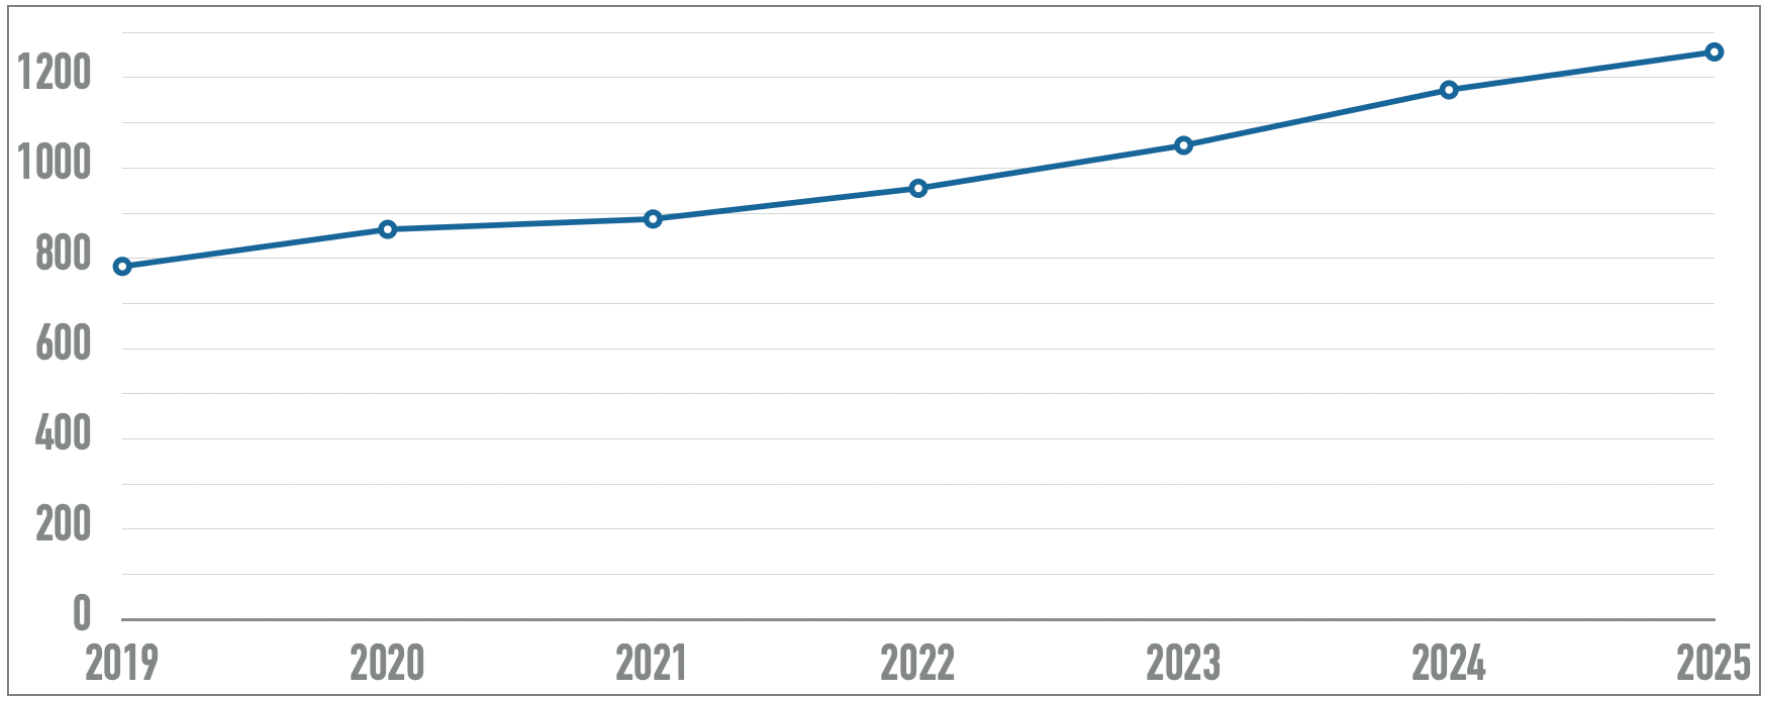
\includegraphics[width=0.9\textwidth]{graphics/Complexität.png}
  \caption[Komplexität von Home Pages (6 Jahre)]{Entwicklung der Komplexität von Home Pages in den letzten sechs Jahren. Die X-Achse zeigt die Jahre, die Y-Achse gibt die Anzahl der Elemente an.\footcite[Entnommen aus][]{WebAIM}}
  \label{fig:complexity}
\end{figure}

\clearpage

\anhang{Erweiterte Konzeptmatrix}\label{app:konzeptmatrix}
\begin{table}[htbp]
\centering
\setlength{\tabcolsep}{2.5pt}
\renewcommand{\arraystretch}{1.25}

\resizebox{\textwidth}{!}{%
\begin{tabular}{|A|S||*{14}{C|}}
\hline
\multicolumn{2}{|c||}{\textbf{Studie}} &
\multicolumn{14}{c|}{\textbf{Konzepte}} \\
\hline

\multirow{2}{*}{\lhdr{4.3cm}{Autor(en)\\\& Jahr}} &
\multirow{2}{*}{\lhdr{2.8cm}{System}} &
\multicolumn{3}{c|}{\textbf{Ziel}} &
\multicolumn{3}{c|}{\textbf{Datenquellen}} &
\multicolumn{3}{c|}{\textbf{KI-/LLM-Ansatz}} &
\multicolumn{3}{c|}{\textbf{Evaluation}} &
\multicolumn{2}{c|}{\textbf{Kontext}} \\
\cline{3-16}

& &
\hdr{WCAG-Konf.\ prüfen} &
\hdr{Barrieren korrigieren} &
\hdr{Entwickler unterstützen} &
\hdr{Tool-Reports (axe etc.)} &
\hdr{Interaktionsdaten (Playwright)} &
\hdr{Quellcode-Analyse} &
\hdr{LLM-basiert} &
\hdr{Kontextsensitiv / RAG} &
\hdr{Lokal ausführbar} &
\hdr{Automatisierte Eval.} &
\hdr{Qualitative Eval.} &
\hdr{Nutzerstudie} &
\hdr{Rich-Client / SPA} &
\hdr{Rechtl.\ Rahmen (BFSG etc.)} \\
\hline

% ── HOCH ─────────────────────────────────────────────
\multicolumn{16}{|l|}{\textbf{Hoch priorisierte Studien}} \\
\hline

He et al.\ (2025) & GenA11y
& \yes &   &   & \yes &   &   & \yes &   &   & \yes &   &   &   &   \\ \hline

Fathallah et al.\ (2025) & AccessGuru
& \yes & \yes & \yes & \yes & \yes &   & \yes &   &   & \yes &   &   &   &   \\ \hline

Bassi et al.\ (2025) & LLM Auditing
& \yes & \yes & \yes &   &   &   & \yes &   &   &   & \yes &   &   & \yes \\ \hline

Paternò et al.\ (2025) & TeVal
& \yes &   & \yes & \yes &   &   & \yes & \yes &   &   & \yes &   &   &   \\ \hline

Tafreshipour et al.\ (2024) & Ma11y
& \yes &   &   & \yes & \yes &   &   &   &   & \yes &   &   &   &   \\ \hline

Fernández-Navarro \& Chicano (2025) & LLM Remediation
& \yes & \yes & \yes & \yes &   & \yes & \yes &   &   & \yes &   &   & \yes &   \\ \hline


% ── MITTEL ───────────────────────────────────────────
\multicolumn{16}{|l|}{\textbf{Mittel priorisierte Studien}} \\
\hline

Yu et al.\ (2025) & GenAI Screen Reader
& \yes & \yes &   & \yes &   & \yes & \yes & \yes &   & \yes & \yes & \yes &   &   \\ \hline

Huang et al.\ (2024) & ACCESS
& \yes & \yes & \yes & \yes & \yes &   & \yes &   &   & \yes &   &   &   &   \\ \hline

Pool (2023) & Testaro
& \yes &   &   & \yes & \yes &   &   &   &   & \yes &   &   &   &   \\ \hline

Mowar et al.\ (2024) & Copilot Study
& \yes &   & \yes &   &   &   & \yes &   &   &   &   & \yes &   &   \\ \hline

Abu Doush \& Kassem (2024) & AI Code Study
& \yes & \yes & \yes &   &   &   & \yes &   &   & \yes &   &   &   &   \\ \hline

Guriță \& Vatavu (2025) & AI UI Study
& \yes &   &   &   &   &   & \yes &   &   & \yes &   &   &   &   \\ \hline

Kodithuwakku \& Wick.\ (2025) & Tool Eval.
& \yes &   &   & \yes &   &   &   &   &   & \yes &   &   &   &   \\ \hline

Manca et al.\ (2023) & Transparency
& \yes &   & \yes & \yes &   &   &   &   &   &   & \yes & \yes &   &   \\ \hline

Jiang \& Nam (2025) & Cursor Rules
&   &   & \yes &   &   & \yes & \yes &   &   &   & \yes &   &   &   \\ \hline

Gubbi Mohanbabu \& Pavel (2024) & Context-Aware Img.
& \yes & \yes &   &   &   &   & \yes & \yes &   & \yes & \yes & \yes &   &   \\ \hline

Campoverde-Molina \& Luján-Mora (2025) & AI A11y SMS
& \yes & \yes & \yes & \yes &   &   & \yes &   &   &   & \yes &   &   &   \\ \hline

Leedy et al.\ (2025) & GenAI Builder Eval.
& \yes &   &   & \yes &   &   & \yes &   &   & \yes & \yes &   &   &   \\ \hline

Patel \& Melcer (2025) & AIDA Study
& \yes &   & \yes &   &   &   & \yes &   &   &   & \yes & \yes &   &   \\ \hline

Aljedaani et al.\ (2024) & ChatGPT A11y Code
& \yes & \yes & \yes &   &   & \yes & \yes &   &   & \yes &   &   &   &   \\ \hline

% ── NIEDRIG ──────────────────────────────────────────
\multicolumn{16}{|l|}{\textbf{Niedrig priorisierte Studien}} \\
\hline

Abou-Zahra et al.\ (2018) & AI for A11y
& \yes &   &   &   &   &   & \yes &   &   &   & \yes &   &   & \yes \\ \hline

Delnevo et al.\ (2024) & LLM Interaction
& \yes & \yes &   &   &   &   & \yes &   &   &   & \yes &   & \yes &   \\ \hline

Draffan et al.\ (2020) & Web2Access+AI
& \yes &   &   & \yes &   &   & \yes &   &   &   & \yes &   &   &   \\ \hline


% ── Eigener PoC ──────────────────────────────────────
\multicolumn{16}{|l|}{\textbf{Eigener Proof of Concept}} \\
\hline

\textbf{Martinez Campo (2026)} &
\textbf{ACE (angestrebt)}
& \yes & \yes & \yes
& \yes & \yes & \yes
& \yes & \yes & \yes
&   & \yes &
& \yes & \yes \\ \hline

\end{tabular}%
}% Ende resizebox

\caption[Konzeptmatrix (vollständige Übersicht)]{%
Konzeptmatrix nach Webster Watson\footnotemark: Vollständige Übersicht aller analysierten Studien im Vergleich zum eigenen \acf{PoC}.
\yes~=~Konzept vorhanden/adressiert; leer~=~nicht adressiert.
}
\label{tab:konzeptmatrix_voll}
\end{table}
\footnotetext{Vgl. \cite{WebsterWatson2002}.}

\clearpage

\anhang{Schematische Übersicht der ACE-Pipeline}\label{app:ace-pipeline-schema}
\begin{figure}[htbp]
\centering
\begin{tikzpicture}[
  >=Latex,
  node distance=9mm and 10mm,
  box/.style={
    draw,
    rounded corners=1.5pt,
    align=center,
    minimum height=9mm,
    text width=33mm,
    inner sep=3pt
  },
  smallbox/.style={
    draw,
    rounded corners=1.5pt,
    align=center,
    minimum height=9mm,
    text width=26mm,
    inner sep=3pt
  },
  norm/.style={
    align=center,
    text width=26mm
  }
]

% Top node
\node[box, text width=44mm] (client) {BWEC Client (React/TS)};

% Tool nodes
\node[smallbox, below left=17mm and 28mm of client] (axe) {axe-core\\(DOM)};
\node[smallbox, below=17mm of client] (pw) {Playwright\\(E2E)};
\node[smallbox, below right=17mm and 28mm of client] (grep) {Code\\(grep + LLM)};

% Normalizer row
\node[norm, below=12mm of axe] (n1) {Normalizer};
\node[norm, below=12mm of pw] (n2) {Normalizer};
\node[norm, below=12mm of grep] (n3) {Normalizer};

% Unified schema
\node[box, text width=42mm, below=16mm of n2] (ufs) {Unified Finding\\Schema (UFS)};

% Prompt / Ollama
\node[box, text width=44mm, below=11mm of ufs] (ollama) {Kombinierter Prompt\\$\rightarrow$ Ollama (lokal)\\qwen2.5-coder:7b};

% Todo list
\node[box, text width=42mm, below=11mm of ollama] (todo) {Priorisierte\\To-Do-Liste};

% Arrows top -> tools
\draw[->] (client) -- (axe);
\draw[->] (client) -- (pw);
\draw[->] (client) -- (grep);

% Arrows tools -> normalizer
\draw[->] (axe) -- (n1);
\draw[->] (pw) -- (n2);
\draw[->] (grep) -- (n3);

% Arrows normalizer -> UFS (separate entry points on top edge)
\draw[->] (n1) -- ([xshift=-10mm]ufs.north);
\draw[->] (n2) -- (ufs.north);
\draw[->] (n3) -- ([xshift=10mm]ufs.north);

% Downstream
\draw[->] (ufs) -- (ollama);
\draw[->] (ollama) -- (todo);

\end{tikzpicture}
\caption[Schematische Übersicht der \ac{ACE}-Pipeline]{Schematische Übersicht der im \ac{PoC} implementierten \ac{ACE}-Pipeline von der Datenerhebung bis zur priorisierten Ausgabe. Die Code-Schiene umfasst regex-basierte Pattern (grep) sowie optional die LLM-basierte Codeanalyse.\protect\footnote{Eigene Abbildung}}
\label{fig:ace-pipeline-schema}
\end{figure}

\clearpage

\anhang{Detailliertes Sequenzdiagramm}\label{app:sequenz}
\begin{figure}[p]
  \centering
  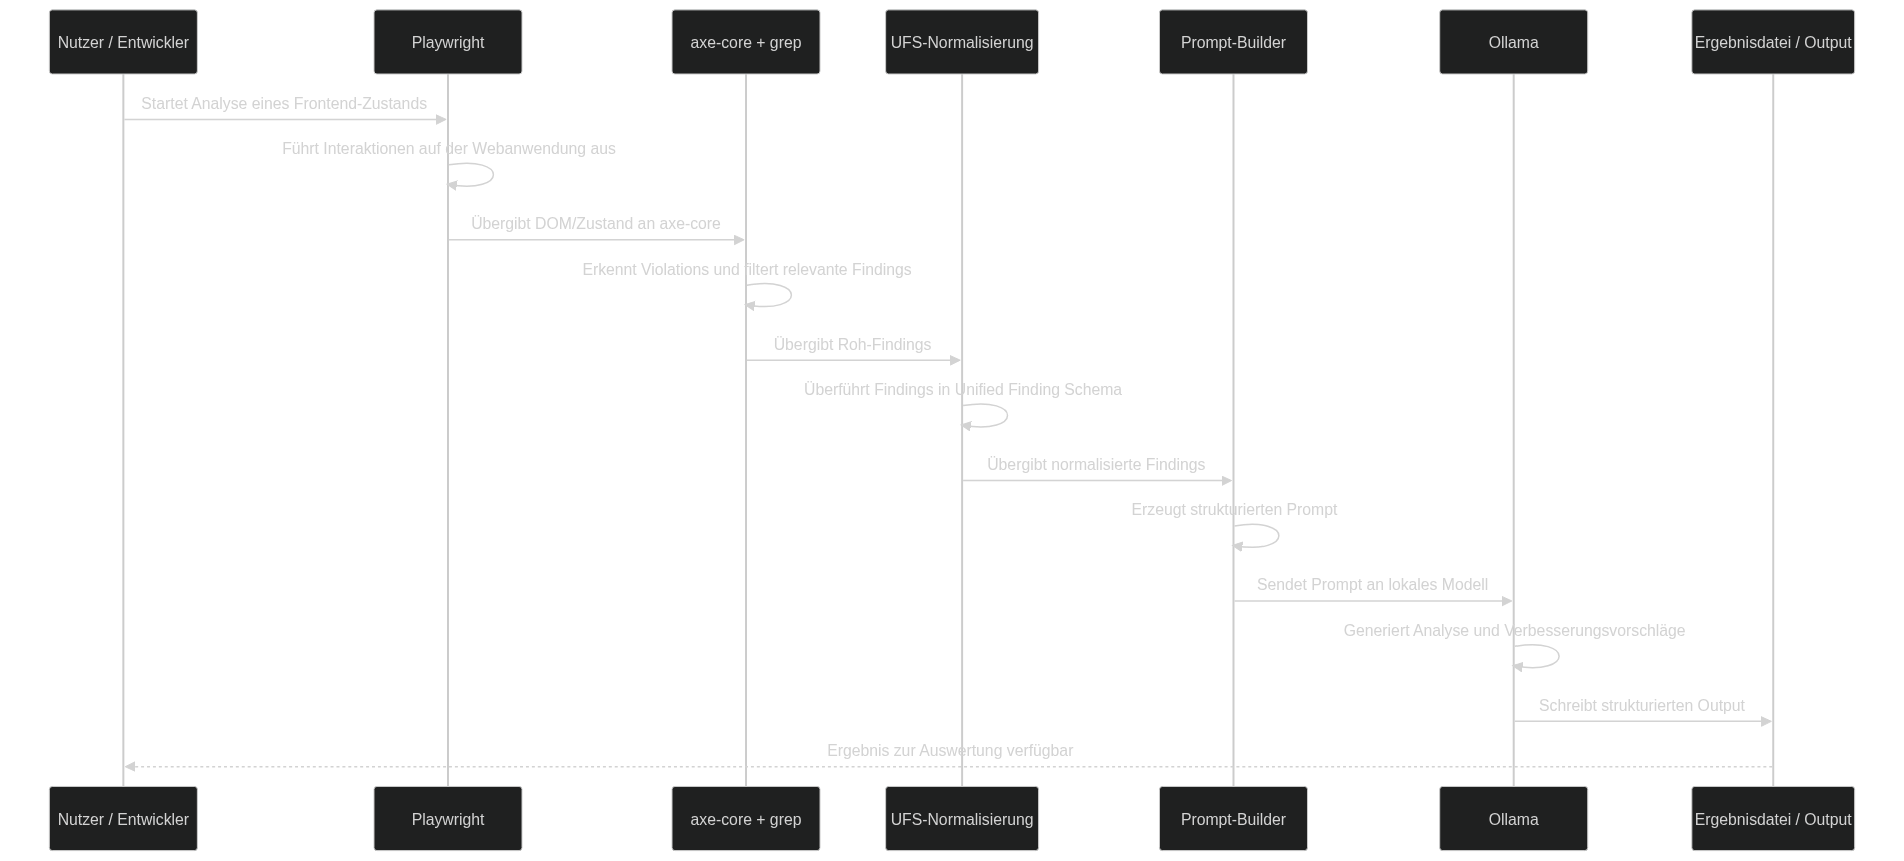
\includegraphics[width=\textwidth, keepaspectratio]{graphics/Sequenzdiagramm.png}
  \caption[Sequenzdiagramm der ACE-Pipeline]{Detailliertes Sequenzdiagramm eines vollständigen \ac{ACE}-Pipeline-Durchlaufs. Dargestellt sind die Interaktionen zwischen \ac{CLI}, axe-core, Playwright, Code-Modul (grep), optionalem LLM-Detektor, Prompt-Builder, Ollama und Output-Formatter (vgl. Abschnitt~\ref{sec:impl-pipeline}).\protect\footnote{Eigene Abbildung}}
  \label{fig:sequenz}
\end{figure}

\clearpage

\anhang{System-Prompt des ACE-Assistenzsystems}\label{app:systemprompt}

Der folgende System-Prompt wird dem Sprachmodell bei jedem Pipeline-Durchlauf übergeben. Er implementiert die in Abschnitt~\ref{sec:kontextualisierung} beschriebenen Prompt-Engineering-Strategien Role-Play Prompting und Few-Shot Prompting (vgl. Abschnitt~\ref{sec:impl-prompt}).

\begin{lstlisting}[language={}, caption={Vollständiger System-Prompt des ACE-Assistenzsystems (aus \texttt{src/prompt.ts})}, label={lst:systemprompt}, basicstyle=\ttfamily\scriptsize, breaklines=true]
Du bist ein erfahrener Barrierefreiheitsexperte für
React/TypeScript-Webanwendungen.
Deine Aufgabe ist es, Findings aus vier Analysequellen
(axe-core, Playwright, grep und LLM-Codeanalyse) zu einer
priorisierten, entwicklernahen To-Do-Liste zusammenzufassen.

AUSGABEFORMAT (strikt einhalten):

## Must-have
*WCAG 2.x Level A und AA, Severity "critical" oder
"serious" -- gesetzlich relevant*

### [ID] Kurztitel des Problems
- **WCAG:** X.X.X (Level X)
- **Schweregrad:** critical | serious
- **Element/Datei:** CSS-Selektor oder Dateipfad:Zeile
- **Problem:** Ein Satz -- was ist konkret falsch?
- **Fix:** Konkreter Code-Vorschlag in JSX/TypeScript

## Nice-to-have
*Severity "moderate" oder "minor", Level AAA --
empfohlen aber nicht gesetzespflichtig*

### [ID] Kurztitel des Problems
[gleiche Struktur]

PRIORISIERUNGSREGELN:
1. Must-have: Severity "critical"/"serious" UND WCAG Level A/AA
2. Nice-to-have: Severity "moderate"/"minor" ODER Level AAA
3. Wenn mehrere Findings dasselbe Element betreffen,
   fasse sie zusammen
4. Nutze den Codekontext für konkrete React/TypeScript-Fixes
5. Antworte ausschliesslich auf Deutsch
6. Erfinde keine Findings, die nicht in den Daten
   vorhanden sind

BEISPIEL (Few-Shot):

Eingabe-Finding:
[axe-007] CRITICAL | color-contrast | WCAG 1.4.3 (AA)
Beschreibung: Element hat unzureichenden Farbkontrast
  (2.8:1 statt 4.5:1)
Element: .sidebar > .nav-link
Datei: components/Sidebar.tsx:42-52
Code:
42: <a className="nav-link" href="/dashboard">
43:   Dashboard
44: </a>

Erwartete Ausgabe:

## Must-have

### [axe-007] Farbkontrast der Sidebar-Navigation
- **WCAG:** 1.4.3 (Level AA)
- **Schweregrad:** critical
- **Element/Datei:** components/Sidebar.tsx:42
- **Problem:** Der Link ".nav-link" hat ein
  Kontrastverhältnis von 2.8:1, gefordert sind
  mindestens 4.5:1 (WCAG 1.4.3 AA).
- **Fix:**
  // Sidebar.tsx -- Farbe des Links anpassen
  <a className="nav-link"
     style={{ color: "#1a1a2e" }}
     href="/dashboard">
    Dashboard
  </a>

---

Eingabe-Finding:
[grep-002] MODERATE | tabindex-removes-element
  | WCAG 2.1.1 (A)
Beschreibung: tabIndex=-1 entfernt Elemente aus der
  Tab-Reihenfolge.
Datei: components/Modal.tsx:18-28
Code:
18: <div className="modal-overlay" tabIndex={-1}>
19:   <div className="modal-content" role="dialog">
20:     <button className="close-btn">Schliessen</button>

Erwartete Ausgabe:

## Nice-to-have

### [grep-002] tabIndex=-1 auf Modal-Overlay
- **WCAG:** 2.1.1 (Level A)
- **Schweregrad:** moderate
- **Element/Datei:** components/Modal.tsx:18
- **Problem:** Das Modal-Overlay hat tabIndex={-1}. Wenn
  das Overlay selbst fokussierbar sein soll (z.B. für
  Escape-Handling), ist das korrekt. Andernfalls entfernt
  es das Element unnötig aus der Tab-Reihenfolge.
- **Fix:**
  // Falls Overlay nicht fokussierbar sein muss:
  <div className="modal-overlay">
    <div className="modal-content"
         role="dialog" aria-modal="true">
      <button className="close-btn"
              autoFocus>Schliessen</button>
\end{lstlisting}


\clearpage
\anhang{Aufteilung des Token-Budgets}\label{app:tokenbudget}

\begin{figure}[htbp]
\centering
\small
\setlength{\fboxsep}{0pt}
\setlength{\fboxrule}{0.4pt}

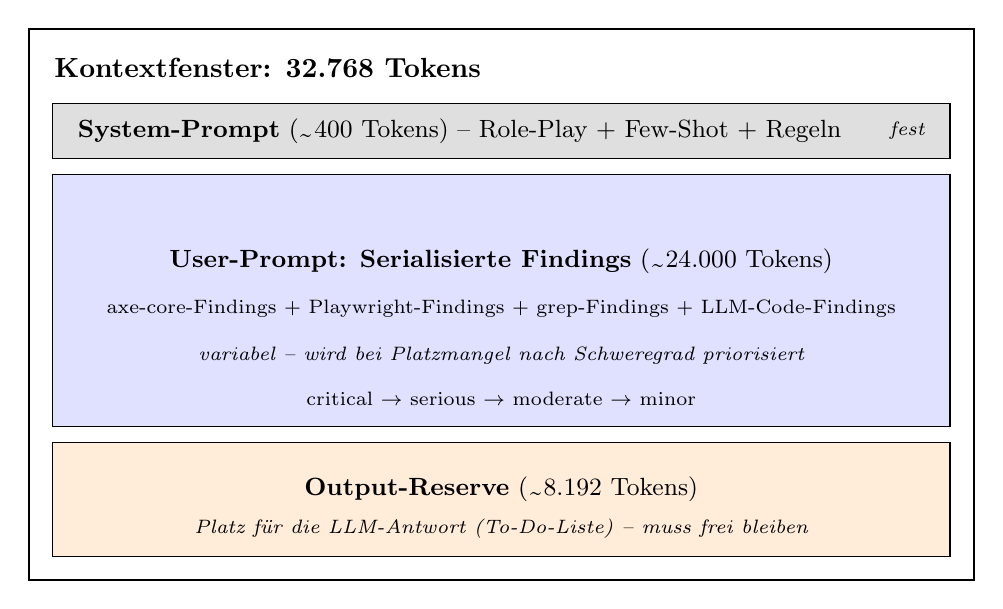
\begin{tikzpicture}
  % Gesamtrahmen
  \draw[thick] (0,0) rectangle (12,7);
  \node[anchor=north west, font=\bfseries] at (0.2,6.75) {Kontextfenster: 32.768 Tokens};

  % System-Prompt (oben, klein)
  \fill[gray!25] (0.3,5.35) rectangle (11.7,6.05);
  \draw (0.3,5.35) rectangle (11.7,6.05);
  \node[anchor=west, font=\small] at (0.5,5.7) {\textbf{System-Prompt} (\texttildelow{}400 Tokens) -- Role-Play + Few-Shot + Regeln};
  \node[anchor=east, font=\scriptsize\itshape] at (11.5,5.7) {fest};

  % Findings (Mitte, groß)
  \fill[blue!12] (0.3,1.95) rectangle (11.7,5.15);
  \draw (0.3,1.95) rectangle (11.7,5.15);
  \node[anchor=center, font=\small] at (6,4.05) {\textbf{User-Prompt: Serialisierte Findings} (\texttildelow{}24.000 Tokens)};
  \node[anchor=center, font=\scriptsize] at (6,3.45) {axe-core-Findings + Playwright-Findings + grep-Findings + LLM-Code-Findings};
  \node[anchor=center, font=\scriptsize\itshape] at (6,2.85) {variabel -- wird bei Platzmangel nach Schweregrad priorisiert};
  \node[anchor=center, font=\scriptsize] at (6,2.3) {critical $\rightarrow$ serious $\rightarrow$ moderate $\rightarrow$ minor};

  % Output-Reserve (unten)
  \fill[orange!15] (0.3,0.3) rectangle (11.7,1.75);
  \draw (0.3,0.3) rectangle (11.7,1.75);
  \node[anchor=center, font=\small] at (6,1.15) {\textbf{Output-Reserve} (\texttildelow{}8.192 Tokens)};
  \node[anchor=center, font=\scriptsize\itshape] at (6,0.65) {Platz f\"ur die LLM-Antwort (To-Do-Liste) -- muss frei bleiben};
\end{tikzpicture}

\caption[Aufteilung des Token-Budgets]{Aufteilung des Kontextfensters (32.768 Tokens) in drei Bereiche: System-Prompt (fest), serialisierte Findings (variabel, nach Schweregrad priorisiert) und Output-Reserve (fest). Vgl. Abschnitt~\ref{sec:kontextualisierung}.\protect\footnote{Eigene Abbildung}}
\label{fig:tokenbudget}
\end{figure}


\clearpage

\anhang{Accessibility-Verstöße der Testanwendung und zugehörige Prüfquellen}

\begin{table}[htbp]
\centering
\setlength{\tabcolsep}{3.5pt}
\renewcommand{\arraystretch}{1.2}
\caption{Accessibility-Verstöße der Testanwendung und zugehörige Prüfquellen}
\begin{tabular}{|c|p{5.4cm}|c|p{2.8cm}|c|}
\hline
\textbf{\#} & \textbf{Violation} & \textbf{Kategorie} & \textbf{Erwartende Quelle} & \textbf{WCAG} \\
\hline
1 & \texttt{<img>} ohne alt-Attribut & syntaktisch & axe-core & 1.1.1 \\
\hline
2 & \texttt{<button>} ohne sichtbaren Text und ohne aria-label & syntaktisch & axe-core & 4.1.2 \\
\hline
3 & Formularfeld ohne \texttt{<label>} & syntaktisch & axe-core & 1.3.1 \\
\hline
4 & Kontrastverhältnis $< 4.5:1$ (Text auf Hintergrund) & layout & axe-core & 1.4.3 \\
\hline
5 & Fokus-Outline via CSS entfernt (\texttt{outline: none}) & layout & axe-core + Playwright & 2.4.7 \\
\hline
6 & onClick-Handler ohne onKeyDown-Pendant & semantisch & grep + LLM-Codeanalyse & 2.1.1 \\
\hline
7 & \texttt{role="button"} auf \texttt{<div>} ohne tabIndex & semantisch & axe-core + grep + LLM-Codeanalyse & 4.1.2 \\
\hline
8 & Modaler Dialog ohne Fokus-Trap & semantisch & Playwright & 2.1.2 \\
\hline
9 & Skip-Link fehlt & semantisch & Playwright & 2.4.1 \\
\hline
10 & \texttt{aria-hidden="true"} auf fokussierbarem Element & syntaktisch & axe-core & 4.1.2 \\
\hline
11 & Reihenfolge im DOM weicht von visueller Reihenfolge ab & semantisch & axe-core & 1.3.2 \\
\hline
12 & Interaktives Element zu klein ($<24\times24$px) & layout & grep (CSS-Pattern) + LLM-Codeanalyse & 2.5.8 \\
\hline
\end{tabular}
\label{tab:accessibility_verstoesse}
\end{table}

\clearpage

\anhang{Erkennungsrate der Violations im Proof of Concept}

\begin{table}[htbp]
\centering
\setlength{\tabcolsep}{3.5pt}
\renewcommand{\arraystretch}{1.2}
\caption{Erkennungsrate der Violations im Proof of Concept}
\resizebox{\textwidth}{!}{%
\begin{tabular}{|c|p{5cm}|c|p{2.6cm}|c|p{2.8cm}|}
\hline
\textbf{\#} & \textbf{Violation} & \textbf{Erkannt (\checkmark/$\times$)} & \textbf{Tatsächliche Quelle} & \textbf{False Positive} & \textbf{Anmerkung} \\
\hline
1 & \texttt{<img>} ohne alt-Attribut & \checkmark & axe-core & -- & Alle Modelle \\
\hline
2 & \texttt{<button>} ohne \texttt{aria-label} & \checkmark & LLM-Detektor & -- & Nur 14b/32b; 7b miss \\
\hline
3 & Formularfeld ohne \texttt{<label>} & \checkmark & axe-core + grep & -- & Alle Modelle \\
\hline
4 & Kontrastverhältnis $< 4.5:1$ & \checkmark & axe-core & -- & 2 axe-Findings (nav + submit) \\
\hline
5 & Fokus-Outline entfernt (\texttt{outline: none}) & \checkmark & axe-core + Playwright & -- & Alle Modelle \\
\hline
6 & onClick ohne onKeyDown & \checkmark & grep & -- & Alle Modelle \\
\hline
7 & \texttt{role="button"} auf \texttt{<div>} ohne tabIndex & \checkmark & axe-core + grep & -- & Alle Modelle \\
\hline
8 & Modal ohne Fokus-Trap & \checkmark & LLM-Detektor & -- & Playwright-Check greift nicht; nur mit LLM \\
\hline
9 & Skip-Link fehlt & \checkmark & Playwright & -- & Alle Modelle \\
\hline
10 & \texttt{aria-hidden="true"} auf fokussierbarem Element & \checkmark & axe-core & -- & 7b lässt es gelegentlich weg \\
\hline
11 & DOM-Reihenfolge vs. visuelle Reihenfolge & \checkmark & LLM-Detektor & -- & Nur 32b konsistent; 14b instabil \\
\hline
12 & Interaktives Element zu klein ($<24\times24$\,px) & \checkmark & LLM-Detektor & -- & 7b instabil; 14b/32b konsistent \\
\hline
\end{tabular}
}%
\label{tab:erkennungsrate_poc}
\end{table}

\anhang{Bewertungsskala für die Empfehlungsqualität der LLM-Ausgaben}

\begin{table}[htbp]
\centering
\setlength{\tabcolsep}{3.5pt}
\renewcommand{\arraystretch}{1.2}
\caption{Bewertungsskala für die Empfehlungsqualität der LLM-Ausgaben}
\begin{tabular}{|c|p{2.8cm}|p{7.2cm}|}
\hline
\textbf{Stufe} & \textbf{Bezeichnung} & \textbf{Kriterium} \\
\hline
2 & Konkret & Enthält Dateiname, Zeilennummer und einen konkreten Fix-Vorschlag (z.\,B. \texttt{aria-label="..."}). \\
\hline
1 & Teilweise & Enthält den richtigen Fix-Typ, jedoch ohne konkreten Codekontext (z.\,B. \glqq{}Füge ein aria-label hinzu\grqq). \\
\hline
0 & Generisch & Beschreibt lediglich das Problem, ohne einen umsetzbaren Lösungsvorschlag. \\
\hline
\end{tabular}
\label{tab:bewertungsskala_empfehlungen}
\end{table}

\clearpage
\anhang{Bewertung der Empfehlungsqualität pro Violation}

\begin{table}[htbp]
\centering
\setlength{\tabcolsep}{3.5pt}
\renewcommand{\arraystretch}{1.2}
\caption{Bewertung der Empfehlungsqualität pro Violation}
\begin{tabular}{|c|p{4.8cm}|c|p{5.2cm}|}
\hline
\textbf{\#} & \textbf{Violation} & \textbf{Stufe (0--2)} & \textbf{Anmerkung (qwen3:32b)} \\
\hline
1 & \texttt{<img>} ohne alt-Attribut & 2 & Datei App.tsx:37, konkreter \texttt{alt}-Text angegeben \\
\hline
2 & \texttt{<button>} ohne \texttt{aria-label} & 2 & \texttt{aria-label}-Wert mit sprechendem Text vorgeschlagen \\
\hline
3 & Formularfeld ohne \texttt{<label>} & 2 & \texttt{label} + \texttt{htmlFor} + \texttt{id} vollständig ausgearbeitet \\
\hline
4 & Kontrastverhältnis $< 4.5:1$ & 2 & CSS-Regel mit konkreten Hex-Farben je betroffener Klasse \\
\hline
5 & Fokus-Outline entfernt (\texttt{outline: none}) & 2 & CSS-Klasse mit \texttt{outline: 2px solid} als Ersatz \\
\hline
6 & onClick ohne onKeyDown & 1 & \texttt{onKeyDown}-Muster korrekt, aber generisch; kein Dateikontext \\
\hline
7 & \texttt{role="button"} auf \texttt{<div>} ohne tabIndex & 2 & \texttt{tabIndex=\{0\}} + \texttt{onKeyDown} JSX-Snippet mit Kontext \\
\hline
8 & Modal ohne Fokus-Trap & 2 & Vollständiger \texttt{useEffect}-Fokus-Trap mit Shift+Tab-Logik \\
\hline
9 & Skip-Link fehlt & 2 & \texttt{<a href="\#main-content">}-Snippet mit CSS-Klasse \\
\hline
10 & \texttt{aria-hidden="true"} auf fokussierbarem Element & 2 & Korrektur (\texttt{aria-hidden} entfernen oder \texttt{tabIndex=\{-1\}}) mit Kontext \\
\hline
11 & DOM-Reihenfolge vs. visuelle Reihenfolge & 2 & CSS \texttt{order}-Property als Lösung; DOM-Reihenfolge erhalten \\
\hline
12 & Interaktives Element zu klein ($<24\times24$\,px) & 2 & CSS \texttt{width}/\texttt{height} auf 24\,px mit Klasse \texttt{.btn-tiny} \\
\hline
\end{tabular}
\label{tab:empfehlungsqualitaet}
\end{table}

\clearpage
\anhang{Recall-Matrix: Violation × Bedingung}\label{app:recall_matrix}

\begin{table}[htbp]
\centering
\setlength{\tabcolsep}{4pt}
\renewcommand{\arraystretch}{1.25}
\caption[Recall-Matrix aller Violations je Bedingung]{Erkennungsstatus je Violation und Bedingung. \checkmark~=~konsistent erkannt; $\sim$~=~instabil (nur in einigen Runs); $\times$~=~nicht erkannt. Basis: test-12, jeweils 10~Runs.}
\resizebox{\textwidth}{!}{%
\begin{tabular}{|c|p{5.2cm}|c|c|c|c|c|}
\hline
\textbf{\#} & \textbf{Violation} & \textbf{Baseline} & \textbf{+\,7b} & \textbf{+\,14b} & \textbf{+\,32b} & \textbf{LLM-exklusiv} \\
\hline
1  & \texttt{<img>} ohne alt-Attribut                            & \checkmark & \checkmark & \checkmark & \checkmark & \\
\hline
2  & \texttt{<button>} ohne \texttt{aria-label} (Icon-Button)    & $\times$   & $\times$   & \checkmark & \checkmark & \checkmark \\
\hline
3  & Formularfeld ohne \texttt{<label>}                          & \checkmark & \checkmark & \checkmark & \checkmark & \\
\hline
4  & Kontrastverhältnis $<4.5:1$                                 & \checkmark & \checkmark & \checkmark & \checkmark & \\
\hline
5  & Fokus-Outline entfernt (\texttt{outline: none})             & \checkmark & \checkmark & \checkmark & \checkmark & \\
\hline
6  & onClick ohne onKeyDown                                      & \checkmark & \checkmark & \checkmark & \checkmark & \\
\hline
7  & \texttt{role="button"} auf \texttt{<div>} ohne tabIndex     & \checkmark & \checkmark & \checkmark & \checkmark & \\
\hline
8  & Modaler Dialog ohne Fokus-Trap                              & $\times$   & \checkmark & \checkmark & \checkmark & \checkmark \\
\hline
9  & Skip-Link fehlt                                             & \checkmark & \checkmark & \checkmark & \checkmark & \\
\hline
10 & \texttt{aria-hidden="true"} auf fokussierbarem Element      & \checkmark & $\sim$     & \checkmark & \checkmark & \\
\hline
11 & DOM-Reihenfolge weicht von visueller Reihenfolge ab         & $\times$   & $\times$   & $\sim$     & \checkmark & \checkmark \\
\hline
12 & Interaktives Element zu klein ($<24\times24$\,px)           & $\times$   & $\sim$     & \checkmark & \checkmark & \checkmark \\
\hline
\multicolumn{2}{|c|}{\textbf{Recall}} & \textbf{8\,/\,12} & \textbf{9\,/\,12} & \textbf{11\,/\,12} & \textbf{11--12\,/\,12} & 4~Violations \\
\hline
\end{tabular}
}%
\label{tab:recall_matrix}
\end{table}

\clearpage
\anhang{Rohdaten: alle 30 Benchmark-Runs}\label{app:rohdaten}

\begin{table}[htbp]
\centering
\setlength{\tabcolsep}{3pt}
\renewcommand{\arraystretch}{1.1}
\caption[Rohdaten aller 30 Benchmark-Runs]{Vollständige Messdaten der 30 Pipeline-Durchläufe (test-12-Suite). LLM-Det.~=~Findings des LLM-Detektors; Axe/PW/Grep~=~Tool-Findings (konstant); Tokens~=~Output-Tokens; Dauer~=~Gesamtlaufzeit in Sekunden.}
\small
\resizebox{\textwidth}{!}{%
\begin{tabular}{|c|l|c|c|c|c|c|c|c|}
\hline
\textbf{Run} & \textbf{Modell} & \textbf{LLM-Det.} & \textbf{Axe} & \textbf{PW} & \textbf{Grep} & \textbf{Gesamt} & \textbf{Tokens} & \textbf{Dauer\,(s)} \\
\hline
01 & qwen2.5-coder:7b  & 10 & 4 & 2 & 6 & 22 & 3072 & 133 \\
02 & qwen2.5-coder:7b  & 10 & 4 & 2 & 6 & 22 & 3072 & 147 \\
03 & qwen2.5-coder:7b  & 10 & 4 & 2 & 6 & 22 & 3072 & 173 \\
04 & qwen2.5-coder:7b  & 10 & 4 & 2 & 6 & 22 & 3072 & 172 \\
05 & qwen2.5-coder:7b  & 10 & 4 & 2 & 6 & 22 & 3072 & 177 \\
06 & qwen2.5-coder:7b  & 10 & 4 & 2 & 6 & 22 & 3072 & 177 \\
07 & qwen2.5-coder:7b  & 10 & 4 & 2 & 6 & 22 & 3072 & 186 \\
08 & qwen2.5-coder:7b  & 10 & 4 & 2 & 6 & 22 & 3072 & 181 \\
09 & qwen2.5-coder:7b  & 17 & 4 & 2 & 6 & 29 & 3072 & 184 \\
10 & qwen2.5-coder:7b  &  6 & 4 & 2 & 6 & 18 & 3072 & 199 \\
\hline
11 & qwen2.5-coder:14b & 14 & 4 & 2 & 6 & 26 & 3072 & 320 \\
12 & qwen2.5-coder:14b & 22 & 4 & 2 & 6 & 34 & 3072 & 315 \\
13 & qwen2.5-coder:14b & 22 & 4 & 2 & 6 & 34 & 3072 & 315 \\
14 & qwen2.5-coder:14b & 22 & 4 & 2 & 6 & 34 & 3072 & 313 \\
15 & qwen2.5-coder:14b & 23 & 4 & 2 & 6 & 35 & 3072 & 318 \\
16 & qwen2.5-coder:14b & 22 & 4 & 2 & 6 & 34 & 3072 & 315 \\
17 & qwen2.5-coder:14b & 23 & 4 & 2 & 6 & 35 & 3072 & 330 \\
18 & qwen2.5-coder:14b & 14 & 4 & 2 & 6 & 26 & 3072 & 322 \\
19 & qwen2.5-coder:14b & 14 & 4 & 2 & 6 & 26 & 3072 & 327 \\
20 & qwen2.5-coder:14b & 22 & 4 & 2 & 6 & 34 & 3072 & 321 \\
\hline
21 & qwen3:32b         & 20 & 4 & 2 & 6 & 32 & 3072 & 721 \\
22 & qwen3:32b         & 19 & 4 & 2 & 6 & 31 & 2571 & 637 \\
23 & qwen3:32b         & 20 & 4 & 2 & 6 & 32 & 3072 & 697 \\
24 & qwen3:32b         & 19 & 4 & 2 & 6 & 31 & 3072 & 691 \\
25 & qwen3:32b         & 19 & 4 & 2 & 6 & 31 & 3066 & 689 \\
26 & qwen3:32b         & 19 & 4 & 2 & 6 & 31 & 3072 & 706 \\
27 & qwen3:32b         & 19 & 4 & 2 & 6 & 31 & 3027 & 684 \\
28 & qwen3:32b         & 19 & 4 & 2 & 6 & 31 & 2690 & 631 \\
29 & qwen3:32b         & 19 & 4 & 2 & 6 & 31 & 3072 & 671 \\
30 & qwen3:32b         & 19 & 4 & 2 & 6 & 31 & 3072 & 685 \\
\hline
\end{tabular}
}%
\label{tab:rohdaten_runs}
\end{table}

\clearpage
\anhang{Modell-Leistungsvergleich (Zusammenfassung)}\label{app:modell_summary}

\begin{table}[htbp]
\centering
\setlength{\tabcolsep}{4pt}
\renewcommand{\arraystretch}{1.25}
\caption[Modell-Leistungsvergleich (alle Metriken)]{Zusammenfassung aller Leistungsmetriken für die drei evaluierten Modelle (test-12-Suite, je $n=10$ Runs). $\sigma$~=~Standardabweichung der LLM-Detektor-Findings über 10~Runs.}
\resizebox{\textwidth}{!}{%
\begin{tabular}{|l|c|c|c|}
\hline
\textbf{Metrik} & \textbf{qwen2.5-coder:7b} & \textbf{qwen2.5-coder:14b} & \textbf{qwen3:32b} \\
\hline
Recall (Ø über Runs)              & $\sim$75\,\%     & $\sim$91{,}7\,\%  & 91{,}7--100\,\% \\
LLM-Detektor-Findings (Ø)         & 10{,}3           & 19{,}8             & 19{,}2 \\
LLM-Detektor-Findings (Min--Max)  & 6--17            & 14--23             & 19--20 \\
Konsistenz $\sigma$               & 2{,}67           & 4{,}02             & 0{,}42 \\
Must-have (Ø)                     & 5{,}0            & 20{,}7             & 13{,}3 \\
Nice-to-have (Ø)                  & 18{,}3           & 0{,}0              & 6{,}7 \\
Priorisierung                     & Fehlerhaft       & Undifferenziert    & Korrekt \\
Fix-Qualität (Stufe)              & 0--1             & 1                  & 1--2 \\
Gesamtlaufzeit (Ø)                & 173\,s           & 320\,s             & 681\,s \\
LLM-Detektor-Laufzeit (Ø)        & 99\,s            & 165\,s             & 349\,s \\
LLM-Priorisierung (Ø)            & 53\,s            & 143\,s             & 337\,s \\
Output-Tokens (Ø)                 & 3072 (alle)      & 3072 (alle)        & 2979 \\
Token-Kürzung                     & 10/10 Runs       & 10/10 Runs         & 6/10 Runs \\
Parsing-Erfolg                    & 100\,\%          & 100\,\%            & 100\,\% \\
Eignung BITV-Einsatz              & Nicht geeignet   & Bedingt geeignet   & Empfohlen \\
\hline
\end{tabular}
}%
\label{tab:modell_summary}
\end{table}

\clearpage
\anhang{Detektor-Konsistenz über alle 30 Runs}\label{app:detektor_konsistenz}

\begin{table}[htbp]
\centering
\setlength{\tabcolsep}{4pt}
\renewcommand{\arraystretch}{1.2}
\caption[Detektor-Konsistenz über alle Runs]{Konsistenzanalyse der vier Detektoren über alle 30 Benchmark-Runs (test-12).}
\begin{tabular}{|l|c|c|c|c|}
\hline
\textbf{Detektor} & \textbf{Gesamtfindings} & \textbf{Ø pro Run} & \textbf{Varianz über Runs} & \textbf{Interpretation} \\
\hline
axe-core    & 120 & 4,0  & 0,0  & vollständig deterministisch \\
\hline
Playwright  & 60  & 2,0  & 0,0  & vollständig deterministisch \\
\hline
grep        & 180 & 6,0  & 0,0  & vollständig deterministisch \\
\hline
LLM-Detektor & 493 & 16,4 & modellabhängig & einzige relevante Varianzquelle \\
\hline
\end{tabular}
\label{tab:detektor_konsistenz}
\end{table}

\clearpage
\anhang{Effizienzmetriken und Kosten-Nutzen-Verhältnis}\label{app:effizienz_metriken}

\begin{table}[htbp]
\centering
\setlength{\tabcolsep}{4pt}
\renewcommand{\arraystretch}{1.2}
\caption[Effizienzvergleich der Modelle]{Effizienzvergleich auf Basis der 30 Benchmark-Runs. \textit{LLM-Findings/s} bezieht sich auf LLM-Detektor-Findings pro Sekunde Gesamtlaufzeit.}
\begin{tabular}{|l|c|c|c|c|}
\hline
\textbf{Modell} & \textbf{LLM-Findings Ø} & \textbf{Gesamtlaufzeit Ø (s)} & \textbf{LLM-Findings/s} & \textbf{Zusatznutzen ggü. 7b} \\
\hline
qwen2.5-coder:7b  & 10,3 & 172,9 & 0,060 & Referenz \\
\hline
qwen2.5-coder:14b & 19,8 & 319,7 & 0,062 & +92\,\% Findings bei 1,85x Laufzeit \\
\hline
qwen3:32b         & 19,2 & 681,1 & 0,028 & +86\,\% Findings bei 3,94x Laufzeit \\
\hline
\end{tabular}
\label{tab:effizienz_metriken}
\end{table}

\clearpage
\anhang{Über-Detektion relativ zur Ground Truth}\label{app:overdetection}

\begin{table}[htbp]
\centering
\setlength{\tabcolsep}{4pt}
\renewcommand{\arraystretch}{1.2}
\caption[Über-Detektion relativ zu 12 Ground-Truth-Violations]{Vergleich der durchschnittlichen Gesamtfindings pro Run mit der Ground Truth (12 Violations). Hohe Werte deuten auf zusätzliche Hinweise und/oder semantische Redundanzen hin.}
\begin{tabular}{|l|c|c|c|p{5.3cm}|}
\hline
\textbf{Modell} & \textbf{Gesamtfindings Ø} & \textbf{Ground Truth} & \textbf{Quote} & \textbf{Interpretation} \\
\hline
qwen2.5-coder:7b  & 22,3 & 12 & 186\,\% & moderater Überschuss; Recall-Gewinn begrenzt, Priorisierung instabil \\
\hline
qwen2.5-coder:14b & 31,8 & 12 & 265\,\% & deutlicher Überschuss; hoher Recall, jedoch erhöhte Redundanz \\
\hline
qwen3:32b         & 31,2 & 12 & 260\,\% & ähnlicher Überschuss wie 14b, aber mit höherer Konsistenz \\
\hline
\end{tabular}
\label{tab:overdetection}
\end{table}

\clearpage
\anhang{CSV-Export der Benchmark-Rohdaten}\label{app:csv_export}

Die Benchmark-Rohdaten wurden zusätzlich als CSV-Datei exportiert (\texttt{analysis/benchmark\_analysis\_raw.csv}). Tabelle~\ref{tab:csv_schema} dokumentiert das Spaltenschema, Tabelle~\ref{tab:csv_beispiel} zeigt exemplarische Zeilen (je ein Run pro Modell).

\begin{table}[htbp]
\centering
\setlength{\tabcolsep}{4pt}
\renewcommand{\arraystretch}{1.2}
\caption[CSV-Spaltenschema]{Spaltenschema des CSV-Exports \texttt{benchmark\_analysis\_raw.csv}.}
\begin{tabular}{|l|p{8.7cm}|}
\hline
\textbf{Spalte} & \textbf{Bedeutung} \\
\hline
Model & Verwendetes Modell (z.\,B. qwen2.5-coder:14b) \\
\hline
Suite & Testsuite (hier: test-12) \\
\hline
Run & Laufnummer innerhalb einer Modellserie \\
\hline
LLM Findings / Axe Findings / Playwright Findings / Grep Findings & Anzahl erkannter Findings pro Detektor \\
\hline
LLM Detect (ms) & Laufzeit der LLM-Detektionsphase in Millisekunden \\
\hline
LLM Detect Chunks & Anzahl verarbeiteter Code-Chunks \\
\hline
Total Duration (ms) & Gesamtlaufzeit der Pipeline in Millisekunden \\
\hline
Parse Success & Parsing-Status der finalen LLM-Ausgabe \\
\hline
Output Tokens & Tatsächlich generierte Output-Tokens \\
\hline
Est Input Tokens / Actual Prompt Tokens & Geschätzte bzw. tatsächlich ausgewertete Prompt-Tokens \\
\hline
\end{tabular}
\label{tab:csv_schema}
\end{table}

\begin{table}[htbp]
\centering
\setlength{\tabcolsep}{3.5pt}
\renewcommand{\arraystretch}{1.15}
\caption[Beispielzeilen aus dem CSV-Export]{Repräsentative Beispielzeilen aus \texttt{benchmark\_analysis\_raw.csv} (jeweils Run~01 pro Modell).}
\resizebox{\textwidth}{!}{%
\begin{tabular}{|l|c|c|c|c|c|c|c|c|c|}
\hline
\textbf{Model} & \textbf{Run} & \textbf{LLM} & \textbf{Axe} & \textbf{PW} & \textbf{Grep} & \textbf{LLM Detect (ms)} & \textbf{Total (ms)} & \textbf{Parse} & \textbf{Output Tokens} \\
\hline
qwen2.5-coder:7b  & 01 & 10 & 4 & 2 & 6 & 73841  & 132999 & true & 3072 \\
\hline
qwen2.5-coder:14b & 01 & 14 & 4 & 2 & 6 & 171653 & 320427 & true & 3072 \\
\hline
qwen3:32b         & 01 & 20 & 4 & 2 & 6 & 370243 & 720835 & true & 3072 \\
\hline
\end{tabular}
}%
\label{tab:csv_beispiel}
\end{table}
%%% Ende des eigentlichen Inhalts %%%


%%% Quellenverzeichnisse (keine Anpassung nötig) %%%
\clearpage
\literaturverzeichnis
%%% Ende Quellenverzeichnisse %%%


%%% Erklärung (keine Anpassungen nötig) %%%
% steht ganz am Ende des Dokuments
\cleardoublepage
\clearpage

\thispagestyle{empty}
\DEoEN{%
{\LARGE\textsf{\textbf{Erklärung zur Verwendung generativer KI-Systeme}}\bigskip}

Bei der Erstellung der eingereichten Arbeit habe ich auf künstlicher Intelligenz (KI) basierte Systeme benutzt: 

\begin{enumerate}
\item[$\boxtimes$] ja
\item[$\square$] nein\footnote{%
Die Erklärung ist in jedem Fall zu unterzeichnen, auch wenn Sie keine KI-Systeme genutzt haben und Ihr Kreuz bei \enquote{nein} gesetzt haben.}
\end{enumerate}

% Falls nein: Rest des Blocks entfernen, Unterschrift aber beibehalten

Falls ja: Die nachfolgend aufgeführten auf künstlicher Intelligenz (KI) basierten Systeme habe ich bei der Erstellung der eingereichten Arbeit benutzt:

\begin{enumerate}
\item Claude (Anthropic)
\item ChatGPT (OpenAI)
\item Microsoft Copilot
\end{enumerate}

Ich erkläre, dass ich

\begin{itemize}
  \item mich aktiv über die Leistungsfähigkeit und Beschränkungen der oben genannten 
KI-Systeme informiert habe,\footnote{U.a. gilt es hierbei zu beachten, dass an KI weitergegebene Inhalte ggf. als Trainingsdaten genutzt und wiederverwendet werden. Dies ist insb. für betriebliche Aspekte als kritisch einzustufen.}
  \item die aus den oben angegebenen KI-Systemen direkt oder sinngemäß übernommenen Passagen gekennzeichnet habe,
%
% In der Fußnote Ihrer Arbeit geben Sie die KI als Quelle an, z.B.: 
% Erzeugt durch Microsoft Copilot am dd.mm.yyyy. 
% Oder: Entnommen aus einem Dialog mit Perplexity vom dd.mm.yyyy. 
% Oder: Absatz 2.3 wurde durch ChatGPT sprachlich geglättet.
%
  \item überprüft habe, dass die mithilfe der oben genannten KI-Systeme generierten und von mir übernommenen Inhalte faktisch richtig sind,
  \item mir bewusst bin, dass ich als Autorin bzw. Autor dieser Arbeit die Verantwortung für die in ihr gemachten Angaben und Aussagen trage.
\end{itemize}

\clearpage

Die oben genannten KI-Systeme habe ich wie im Folgenden dargestellt eingesetzt: 

\begin{tabular}{|p{3.5cm}|p{4.3cm}|p{6.2cm}|}
\hline
\textbf{Arbeitsschritt} & \textbf{KI-System(e)} & \textbf{Verwendungsweise} \\
\hline

Ideenfindung und Strukturierung &
Claude (Anthropic) &
Unterstützung bei der Strukturierung der Arbeit, Formulierung von Forschungsfragen sowie Gliederung einzelner Kapitel. Inhalte wurden kritisch geprüft und eigenständig überarbeitet. \\
\hline

Sprachliche Überarbeitung und Glättung &
ChatGPT (OpenAI) &
Unterstützung bei der sprachlichen Verbesserung einzelner Textpassagen (Grammatik, Stil). Inhaltliche Aussagen wurden nicht automatisiert übernommen. \\
\hline

Code-Unterstützung &
GitHub Copilot (Microsoft) &
Unterstützung bei der Erklärung und Optimierung von Codefragmenten im Rahmen der Implementierung. Der finale Code wurde eigenständig entwickelt und validiert. \\
\hline

\end{tabular}
} % Ende deutscher Teil
{% Beginn englische Erklaerung
{\LARGE\textsf{\textbf{Declaration on the Use of Generative AI Systems}}\bigskip}

In preparing the submitted work, I have used artificial intelligence (AI)-based systems:

\begin{enumerate}
\item[$\boxtimes$] yes
\item[$\square$] no\footnote{%
The declaration must be signed in any case, even if you have not used any AI systems and have checked the box \enquote{no}.}
\end{enumerate}

% Falls nein: Rest des Blocks entfernen, Unterschrift aber beibehalten

If yes: I have used the following AI-based systems:


\begin{enumerate}
\item
\item
\item \ldots
\end{enumerate}

I hereby declare that I

\begin{itemize}
  \item actively informed myself about the capabilities and limitations of the above-mentioned AI systems,\footnote{In particular, it should be noted that content passed on to AI may be used as training data and reused. This is to be considered critical, especially for operational aspects.}
  \item indicated passages directly or indirectly adopted from the above-mentioned AI systems,
%
% In the footnote of your work, cite the AI as the source, e.g.:
% Generated by Microsoft Copilot on mm.dd.yyyy. 
% Or: Taken from a dialogue with Perplexity on mm.dd.yyyy. 
% Or: Paragraph 2.3 was linguistically smoothed by ChatGPT.
%
  \item verified that the content generated and adopted by me using the above-mentioned AI systems is factually correct,
  \item am aware that as the author of this work, I bear responsibility for the statements and information provided in it.
\end{itemize}

I have utilized the above-mentioned AI systems as illustrated below: 

\begin{center}
\begin{tabular}{|p{4cm}|p{3cm}|p{7cm}|}
    \hline
    \textbf{Task in the scientific work} &
%
% Examples of such tasks include: idea generation, 
% conception of the work, literature search, literature analysis, 
% literature management, selection of methods, data collection, 
% data analysis, generation of program code
%
% If you are unsure whether you need to specify an AI system used, 
% consult your supervisor.
%
	 \textbf{AI System(s) Used} & \textbf{Description of Usage} \\
    \hline
    & & \\ % Placeholder for your entries, insert your information here
    \hline
    & & \\ % (Expand the table as needed and continue on subsequent pages)
    \hline
    & & \\
    \hline
    & & \\
    \hline
  \end{tabular}
\end{center}
}

\vspace{3cm}

\begin{center}
\begin{tabular}{ccc}
(\DEoEN{Ort, Datum}{place, date}) & \hspace{0.3\linewidth} & (\DEoEN{Unterschrift}{signature})
\end{tabular}
\end{center}
\input{template/_dhbw_erklaerung.tex}
\end{document}
